\documentclass[12pt,a4paper,english,twoside]{book}
\usepackage[german,english]{babel}
\usepackage[T1]{fontenc} 
\usepackage[utf8]{inputenc}
\usepackage{amsfonts}
\usepackage{amsmath}
\usepackage{latexsym}
\usepackage{amssymb}
\usepackage{epsfig}
\usepackage{moreverb}
\usepackage{rotating}
\usepackage{enumerate}
\usepackage{graphics, graphicx,wrapfig}
\usepackage{fancybox}
\usepackage{picinpar,varioref,floatflt}
\usepackage{ae}
\usepackage{longtable}
\usepackage{booktabs}
\usepackage{textcomp}
\usepackage{float}
\usepackage{url}
\usepackage{unizhdt}
% newly added
\usepackage{listings}
\usepackage{hyperref}
%\usepackage{parskip}
\usepackage{array}
\usepackage{csquotes}

\makeatletter
\newenvironment{CenteredBox}{% 
\begin{Sbox}}{% Save the content in a box
\end{Sbox}\centerline{\parbox{\wd\@Sbox}{\TheSbox}}}% And output it centered
\makeatother

\usepackage{color}
\usepackage[table,xcdraw]{xcolor}
\definecolor{lightgray}{rgb}{.9,.9,.9}
\definecolor{darkgray}{rgb}{.4,.4,.4}
\definecolor{purple}{rgb}{0.65, 0.12, 0.82}
\definecolor{darkgreen}{RGB}{30, 142, 20}

% \lstdefinelanguage{JavaScript}{
% 	keywords={typeof, new, true, false, catch, function, return, null, catch, switch, let, var, if, in, while, do, else, case, break, async, await, const},
% 	keywordstyle=\color{purple}\bfseries,
% 	ndkeywords={class, export, boolean, throw, implements, import, this},
% 	ndkeywordstyle=\color{darkgray}\bfseries,
% 	identifierstyle=\color{black},
% 	sensitive=false,
% 	comment=[l]{//},
% 	morecomment=[s]{/*}{*/},
% 	commentstyle=\color{darkgreen}\ttfamily,
% 	stringstyle=\color{darkgreen}\ttfamily,
% 	morestring=[b]',
% 	morestring=[b]"
% }

% \lstset{
% 	language=JavaScript,
% 	extendedchars=true,
% 	basicstyle=\footnotesize\ttfamily,
% 	showstringspaces=false,
% 	showspaces=false,
% 	numbers=left,
% 	numberstyle=\footnotesize,
% 	numbersep=9pt,
% 	tabsize=2,
% 	breaklines=true,
% 	showtabs=false,
% 	captionpos=b
% }


% Personal additions regarding code listings
\lstdefinelanguage{Python}{
    keywords={False, None, True, and, as, assert, async, await, break,
              class, continue, def, del, elif, else, except, finally,
              for, from, global, if, import, in, is, lambda, nonlocal,
              not, or, pass, raise, return, try, while, with, yield},
    sensitive=true,
    comment=[l]{\#},
    morecomment=[s]{"""}{"""},
    morecomment=[s]{'''}{'''}, 
    string=[b]{"},
    string=[b]{'},
    morestring=[b]{"},
    morestring=[b]{'},
    alsoletter={_},
}

% Define colors for syntax highlighting
\definecolor{docstringcolor}{rgb}{0.0, 0.5, 0.0}
\definecolor{keywordcolor}{rgb}{0.0, 0.0, 1.0}
\definecolor{functioncolor}{rgb}{0.7, 0.2, 0.2}

% Set up listings
\lstset{
    language=Python,
    basicstyle=\ttfamily,
    keywordstyle=\color{keywordcolor},
    commentstyle=\color{darkgreen},
    stringstyle=\color{docstringcolor},
    numbers=left,
    numberstyle=\footnotesize,
    stepnumber=1,
    numbersep=5pt,
    frame=single,
    breaklines=true,
    backgroundcolor=\color{white},
    showstringspaces=false,
    tabsize=4,
    captionpos=b
}


%%%%%%%%%%%%%%%%%%%%%%%%%%%%%%%%%%%%%%%%%%%%%%%%%%


% Bibliography management
\usepackage[style=numeric-comp,backend=bibtex,urldate=comp,doi=false,isbn=false]{biblatex}
\setcounter{secnumdepth}{3}
\addbibresource{references.bib}
\AtEveryBibitem{
 \clearlist{language}
 \clearfield{note}
 \clearlist{publisher}
 \clearlist{location}
 \clearfield{eprinttype}
 \clearfield{eprint}
 \ifentrytype{misc}{}{
  \clearfield{url}
  \clearfield{urlyear}
 }
}



%%%%%%%%%%%%%%%%%%%%%%%%%%%%%%%%%%%%%%%%%%%%%%%%%%

% Define the language of the diploma thesis
\selectlanguage{english}
%\selectlanguage{german}

\pagestyle{headings}

\begin{document}

%%%%%%%%%%%%%%%%%%%%%%%%%%%%%%%%%%%%%%%%%%%%%%%%%%

% Define the author printed on the cover page
\author{Lennart T\"ollke}
% Define the city and country of the author
\authorcity{Zurich, Switzerland}
% Define the student ID (Matrikelnummer)
\studentid{21-701-735}
% Define the title with optional subtitle
\title{A Solution based on Brain-Computer Interfaces to Mitigate
Cognitive Warfare}
% Define the supervisors
\supervisors{ Dr. Alberto Huertas Celdr\'an, Chao Feng, Dr. Sergio L\'opez Bernal, Victoria L\'opez Madejska, Prof. Dr. Burkhard Stiller}
% Define the submission date
\submissiondate{September 11, 2024}

%%%%%%%%%%%%%%%%%%%%%%%%%%%%%%%%%%%%%%%%%%%%%%%%%%

% Make the title page
\maketitle

% Make the imprint on the back of the cover page
\makeimprint

\pagenumbering{roman}

% Include the files of the diploma thesis
%\cleardoublepage
\chapter*{Declaration of Independence}
\addcontentsline{toc}{chapter}{Declaration of Independence}
I hereby declare that I have composed this work independently and without the use of any aids other than those declared (including generative AI such as ChatGPT). I am aware that I take full responsibility for the scientific character of the submitted text myself, even if AI aids were used and declared (after written confirmation by the supervising professor). All passages taken verbatim or in sense from published or unpublished writings are identified as such. The work has not yet been submitted in the same or similar form or in excerpts as part of another examination.

\vspace{2cm}

Z{\"u}rich, September 11, 2024 \hspace{3cm} \hrulefill \\
\hspace*{8.1cm} Signature of student
\chapter*{Abstract Deutsch}
\addcontentsline{toc}{chapter}{Abstract}


%===============================================================================
%%%%%%%%%%%%%%%%%%%%%%%%%%%%%%%%
% Recipe to do an abstract:
%%%%%%%%%%%%%%%%%%%%%%%%%%%%%%%%
%(1) Context
%(2) Research Gap
%(3) Goals, Objectives
%(4) Methodology, how
%(5) Results

% Example:
%Abstract
%(1) In the context of energy efficiency in computer networks, a significant number of solutions ranging from protocols and functionalities to energy efficiency-oriented management applications have been proposed. 
%(2) However, the characteristics of environments to develop and validate such solutions are not as discussed as the solutions themselves. 
%(3) Considering this, this work proposes an emulation environment to develop and validate energy efficiency-oriented solutions, as well as discuss their specific characteristics. 
%(4) Thus, three functionalities of different network scopes are implemented, Adaptive Link Rate (interface level), Syncronized Coalescing (device level) and SustNMS (network level) in the Mininet emulation environment using the implemented software-defined networks paradigm on the POX controller. 
%(5) The environment is validated by comparing the energy savings achieved by these features in a topology inspired by the National Research Network (RNP).

\selectlanguage{german}

Kognitive Kriegsf\"uhrung ist eine aktuell aufkommende Bedrohung, deren Praktiken auf die Beeinflussung der Kognition des Gegners abzielen. Elektromagnetische Angriffe sind eine technologische Variante dieser Kriegsf\"uhrung, welche die gesunde Gehirnaktivit\"at durch elektromagnetische Strahlung st\"ort. Damit in Verbindung gebrachte Zwischenf\"alle haben gezeigt, dass dies zu einer Reihe von Symptomen wie Kopfschmerzen, Schwindelgef\"uhlen und Ged\"achtnisst\"orungen f\"uhren kann.\\
Trotz der Schwere dieser Angriffe und ihres zunehmenden Bedrohungspotenziales, existieren bisher keine Ans\"atze f\"ur Gegenmassnahmen. Diese Arbeit beinhaltet daher den Versuch, auf Grundlage von Gehirn-Computer-Schnittstellen (BCIs) eine L\"osung zu entwickeln, die die Auswirkungen solcher Angriffe abschw\"achen kann. Der Schwerpunkt liegt dabei auf dem kognitiven Prozess der Ged\"achtniskonsolidierung.\\
Durch Sichtung der verf\"ugbaren Literatur werden elektromagnetische Angriffe und die M\"oglichkeiten von BCIs untersucht. Darauf aufbauend folgen spezifischere Untersuchungen, die mit Hilfe von Gehirnsimulationen durchgef\"uhrt werden.\\
Obwohl es im Rahmen dieser Arbeit nicht m\"oglich ist, eine spezifische Gegenmassnahme vorzuschlagen, findet die Untersuchung notwendiger Aspekte f\"ur deren Entwicklung statt. Insbesondere k\"onnen einige potenziell zugrundeliegende Mechanismen elektromagnetischer Angriffe identifiziert und in die Simulation integriert werden. Daraus ergibt sich eine deutliche Abweichung von gesunder Hirnaktivit\"at, die auch mit den berichteten Beeintr\"achtigungen des Ged\"achtnisses in Verbindung gebracht werden kann.


\newpage

\selectlanguage{english}
\vspace*{50pt} % Add some vertical space before the title
{\Huge\bfseries Abstract English} % Match chapter title formatting
\vspace*{40pt} % Space after the title

%(1) Context
Cognitive Warfare is an emerging threat that encompasses practices to interfere with the adversaries' cognition. Electromagnetic attacks are a technological example of this, where with the help of electromagnetic radiation, normal brain activity is disrupted. This can lead to a range of symptoms like headaches, dizziness, and memory impairments, which were reported from a series of related health incidents.\\
%(2) Research Gap
Even though such attacks occur and their potential threat only seems to increase, no countermeasures have been proposed so far.
%(3) Goals, Objectives
This work therefore tries to develop a solution, based on brain-computer interfaces that could mitigate the effects of such attacks. Focusing specifically on the cognitive process of memory consolidation.\\
%(4) Methodology, how
By reviewing the available literature, electromagnetic attacks and the capabilities of brain-computer interfaces are explored. This is then used to perform more specific investigations with the help of brain simulations.\\
%(5) Results
Whilst no specific countermeasure can be proposed in the scope of this work, necessary aspects for its development are explored. In particular, potential underlying mechanisms of electromagnetic attacks are identified and integrated into the simulation. This results in a clear deviation from healthy brain activity, which can also be associated with the reported memory impairments. 







%\cleardoublepage
\chapter*{Acknowledgments}
\addcontentsline{toc}{chapter}{Acknowledgments}

I would like to express my sincere gratitude to my supervisors, Dr. Alberto Huertas Celdr\'an, Dr. Sergio L\'opez Bernal, and Victoria L\'opez Madejska for their guidance and support throughout this research. Their expertise and valuable feedback during our regular meetings were crucial in shaping the direction of this thesis.\\
I am very thankful for all your insights, the time investment, and your dedication which helped me to overcome challenges and allowed me to complete this work.

Further, I would like to thank Am\'elie Aussel, who contributed a lot to my simulation work, by generously offering valuable help, regarding many aspects of her model.

Finally, I would like to extend my gratitude to Prof. Dr. Burkhard Stiller for allowing me to write my bachelor's thesis at the Communication Systems Group (CSG) of the University of Zurich.

\tableofcontents
\cleardoublepage
\pagenumbering{arabic}
% --------------
% Body
% --------------
\chapter{Introduction}
%
% Use thesis description
%
%The. Introduction:
%I. The introduction of a paper aims to show the objectives, the work and give a view of the subject addressed. This should include:
%1. Contextualisation of the work as a whole. Within this context can be placed the justifications or motivations for the execution of the work (must be consistent with the arguments defined in the project);
%2. An overview of the whole subject matter at work, without going into details or drawing conclusions. This is intended to give an overview of all the content addressed;
%3. Definition of the objectives to be achieved with the work (they must be by what was defined in the project). In some cases (completion work or have 40 pages of content) it is recommended to subdivide the objectives into two categories:
%The. General objective: it is normally defined objective in the project with a bit more complementary information;
%B. Specific objectives: There are several intermediate objectives that must be achieved so that when all of these are achieved, it is possible to meet the general objective.
%4. Explain how the work is organised. This is not to describe the content of the chapter as it is in the index/summary, but to say how and why the work was organised and created in the way it is. It seeks to show the reader the logical meaning of evolution and allow it to judge the best way to read the work;
%5. Explain the method of performing the work. To carry out the work, the student can use several methods of work such as research / bibliographic review, field research, experimentation (empirical or not), etc. It is important to inform about the method because it indicates the reasoning and type of work performed.
%
%II. Looking at the described items that should compose the introduction, it's hard to imagine that it has less than one page;
%
% Cognitive Warfare
    % interference with decision-making process 
        % employing different means
            % Information / disinformation
            % Physical/Technological ones
    % Electromagnetic radiation
        % constitutes the form of interest for this thesis
    % Are associated with Havanna syndrome
        % can cause a wide range of cognitive impairments
% Brain Computer interfaces
    % Enable direct communication between brain/computer
        % through capabilities of detection and stimulation
    % could be used to mitigate effects
The term \textit{cognitive warfare} refers to the practice of interfering with the cognition of human targets \cite{Claverie.2022}. This includes information-based techniques, where with the help of disinformation or propaganda, the victims' beliefs are manipulated \cite{Backes.2019}. But also more fundamental attacks that physiologically interfere with the targets' brain \cite{EADS.2023}.\\
The latter one, and specifically \textit{electromagnetic attacks}, are what this thesis focuses on. Such attacks employ Electromagnetic Radiation (EMR) to alter neurological activity and are associated with the Havana syndrome \cite{Pavlin.2020}. In this context, they led to a range of symptoms including headaches or dizziness, but also persisting impairments in memory and concentration.\\
With the help of \textit{Brain-Computer Interfaces} (BCIs), information can be transferred directly between the brain and devices, which bears a lot of potential for medical applications \cite{NicolasAlonso.2012}. Their advanced capabilities to detect and influence brain activity could however also be used to identify and mitigate electromagnetic attacks \cite{Bernal.2021} \cite{Bernal.2023}.


\section{Motivation}
% Why perform this work
    % What makes it valuable or necessary
% derive from Cognitive warfare/Relevance
Considering, that cognitive warfare is practiced by many states and institutions \cite{Claverie.2022} \cite{Backes.2019}, and that already a series of health incidents were attributed to electromagnetic attacks \cite{Pavlin.2020}, the threat imposed by such technologies should not be underestimated. It is therefore advisable to investigate the topic and related technologies, to be prepared for this imminent threat. Especially since with BCIs, a powerful tool and potential solution could be identified.
% Identification research gap


\section{Thesis Goals}
% What are the objectives of the work
% Countermeasure  based on BCI to mitigate cognitive effects of electromagnetic attacks
    % Requires:
    % Identification, and configuration of suitable simulation model
        % employing realistic topology
        % Produce somewhat realistic healthy behavior
        % representing a cognitive process
    % Integration of electromagnetic attack into the simulation
        % by identifying underlying mechanisms
        % implement them
        % producing significantly altered behavior
    % Development of countermeasure algorithm, that respects the capabilities of BCIs
        % Which can mitigate the effect of attacks
The general goal of this thesis is to design and evaluate a countermeasure, based on BCIs to mitigate the impact of electromagnetic attacks on cognitive processes. To achieve this, intermediate goals were defined, which can be chronologically summarized as follows:
\begin{description}
    \item[The identification of a suitable simulation model:] This model should employ a realistic topology and be related to a relevant cognitive process. It should allow for the simulation of realistic brain activity which provides a measure of performance in the cognitive process.
    \item[The integration of an electromagnetic attack:] This requires a review of the literature on electromagnetic attacks, to identify their underlying mechanisms. Then an attack should be designed based on these mechanisms and integrated into the simulation model. Yielding an altered simulation behavior and output.
    \item[The development of a countermeasure:] Based on the observed effects of electromagnetic attacks, a countermeasure shall be designed, implemented, and evaluated. This countermeasure must respect the capabilities of BCIs and should alleviate the impact of the attack.
\end{description}


\section{Methodology}
% As mentioned research is performed with simulations
    % Where the healthy base case simulation results are compared to alterations like attacks
    % Allowing to observe changes evaluate impact
As mentioned above, the research of this thesis will incorporate multiple methodologies. First, a literature review will be performed to explore realistic neural typologies and electromagnetic attacks.\\
Then a series of experiments will be performed with the help of brain simulations. Their objective will mainly be to observe how the model behavior changes in response to alterations. For example when an electromagnetic attack is integrated. 


\section{Thesis Outline}
% General structure of work
% Intention of structure
    % First present fundamentals and clarify key concepts
    % Identify whats there and the exact research gap
    % Present approach to research and explain theoretical basis of design choices
    % show and explain the implementations that were necessary to perform the research
    % Present the results of simulations and evaluate theri meaning in the large context
The general structure of this thesis is as follows. Starting with chapter \ref{chap:background}, the most important concepts are clarified to establish a theoretical basis for the following work. In chapter \ref{chap:related-work}, these concepts are expanded and specified for the subsequent research, employing simulations. All the necessary information about the more practical simulation work, are however elaborated and summarized in chapter \ref{chap:design}. This includes details regarding the approach and environment of the simulations as well as the theoretical basis for any implementations. After that, the written code, relevant to the contribution of this work is presented and explained in chapter \ref{chap:implementation}. Subsequently, the simulation results are shown and evaluated in chapter \ref{chap:evaluation}. Leaving only the final chapter \ref{chap:considerations}, in which a conclusive overview of the performed work is supplied.
\chapter{Background} %concepts
\label{chap:background}
% Just description of fundamental concepts in which the thesis is built upon. Do not need to list all concepts, but only major ones.
    The following chapter supplies an overview of the fundamental concepts that this thesis is based upon. As a first step, \textit{Neurobiology} is considered as many other topics require a basic understanding of our nervous system. Therefore its most important structures and their functionality are explained. Based on this, \textit{Cognitive Processes} are considered. A focus is thereby laid upon some examples that are of particular interest to this thesis.
    But also, the concept of \textit{Cognitive warfare} is being explored. First supplying a general overview of this rather broad field, followed by a more detailed analysis of NeuroStrikes and their relevance.
    Subsequently, \textit{Brain-Computer Interfaces} and their technological underpinnings are discussed. By presenting a few examples of both invasive and non-invasive methods, their capabilities and potential use cases are revealed.
    Finally, the topic of \textit{Brain Simulations} is introduced and some prominent examples of simulators are discussed, revealing their differences and specific use cases. 


\section{Neurobiology}
    %Overview of the Neurobiological part and relevance for my thesis. -> going from Big structures to small ones and from simple to complex - To be written after subsubsections
    When considering BCIs and electromagnetic attacks, it is essential to have an understanding of the fundamental aspects of neurobiology. Therefore, the brain and its functionality are of central importance for this thesis, which is why this section is dedicated to it. Starting with the bigger and more general structures, it progresses down to the molecular level.

\subsection{The Brain}
%Neurolagical Organisation:
    The Brain is our body's central control organ and enables us to engage in remarkable activities like thinking, planning, talking, and countless more. It is an extremely complex organ, which for the most part is made up of about 86 billion nerve and glial cells. Due to their intricate and compact organization, the brain takes on its distinct, cauliflower-like appearance. Next to its apparent separation into two hemispheres (which take care of the contra-lateral side of the body), scientists further specified four major lobes, that lie on the surface of each hemisphere \cite{thebrain-SimpleToComplex-neuroAnatomy-b}.
    
    \begin{figure}[H]
        \centering
        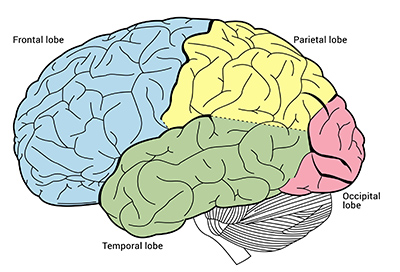
\includegraphics[width=0.5\linewidth]{images/BrainLobes.jpg}
        \caption{The brain's four external lobes \cite{LobesOfBrain}}
        \label{fig:external-lobes}
    \end{figure}

    Although most brain functions require an interplay of many different regions across the entire brain, each lobe can still be made responsible for the bulk of certain functions \cite{LobesOfBrain}. The individual lobes therefore can be associated with the following:
    %
    \begin{description}
    \item[Frontal lobe:] Executive functions like planning, reasoning, and problem-solving. But it is also involved in emotional regulation and what makes up the personality.
    \item[Parietal lobe:] Integration of sensory information, which includes taste, touch, temperature, and pain. Also associates visual and auditory signals with memories.
    \item[Occipital lobe:] Decoding of visual information into form color and movement. Facilitates visual identification of Objects.
    \item[Temporal lobe:] Analyses auditory information and makes it possible to distinguish volume and frequency of sounds.
    \cite{thebrain-SimpleToComplex-neuroAnatomy-b}
    \end{description} 
    
    % If useful/necessary, elaborate on Cerbellum here
    
    Only when a sagittal section of the brain is made (which is a cut through the brain that separates the two hemispheres), do many more important structures become visible. For example the cingulate gyrus, as well as other parts of the limbic system \cite{thebrain-SimpleToComplex-neuroAnatomy-i}.
    
    \begin{figure}[H]
        \centering
        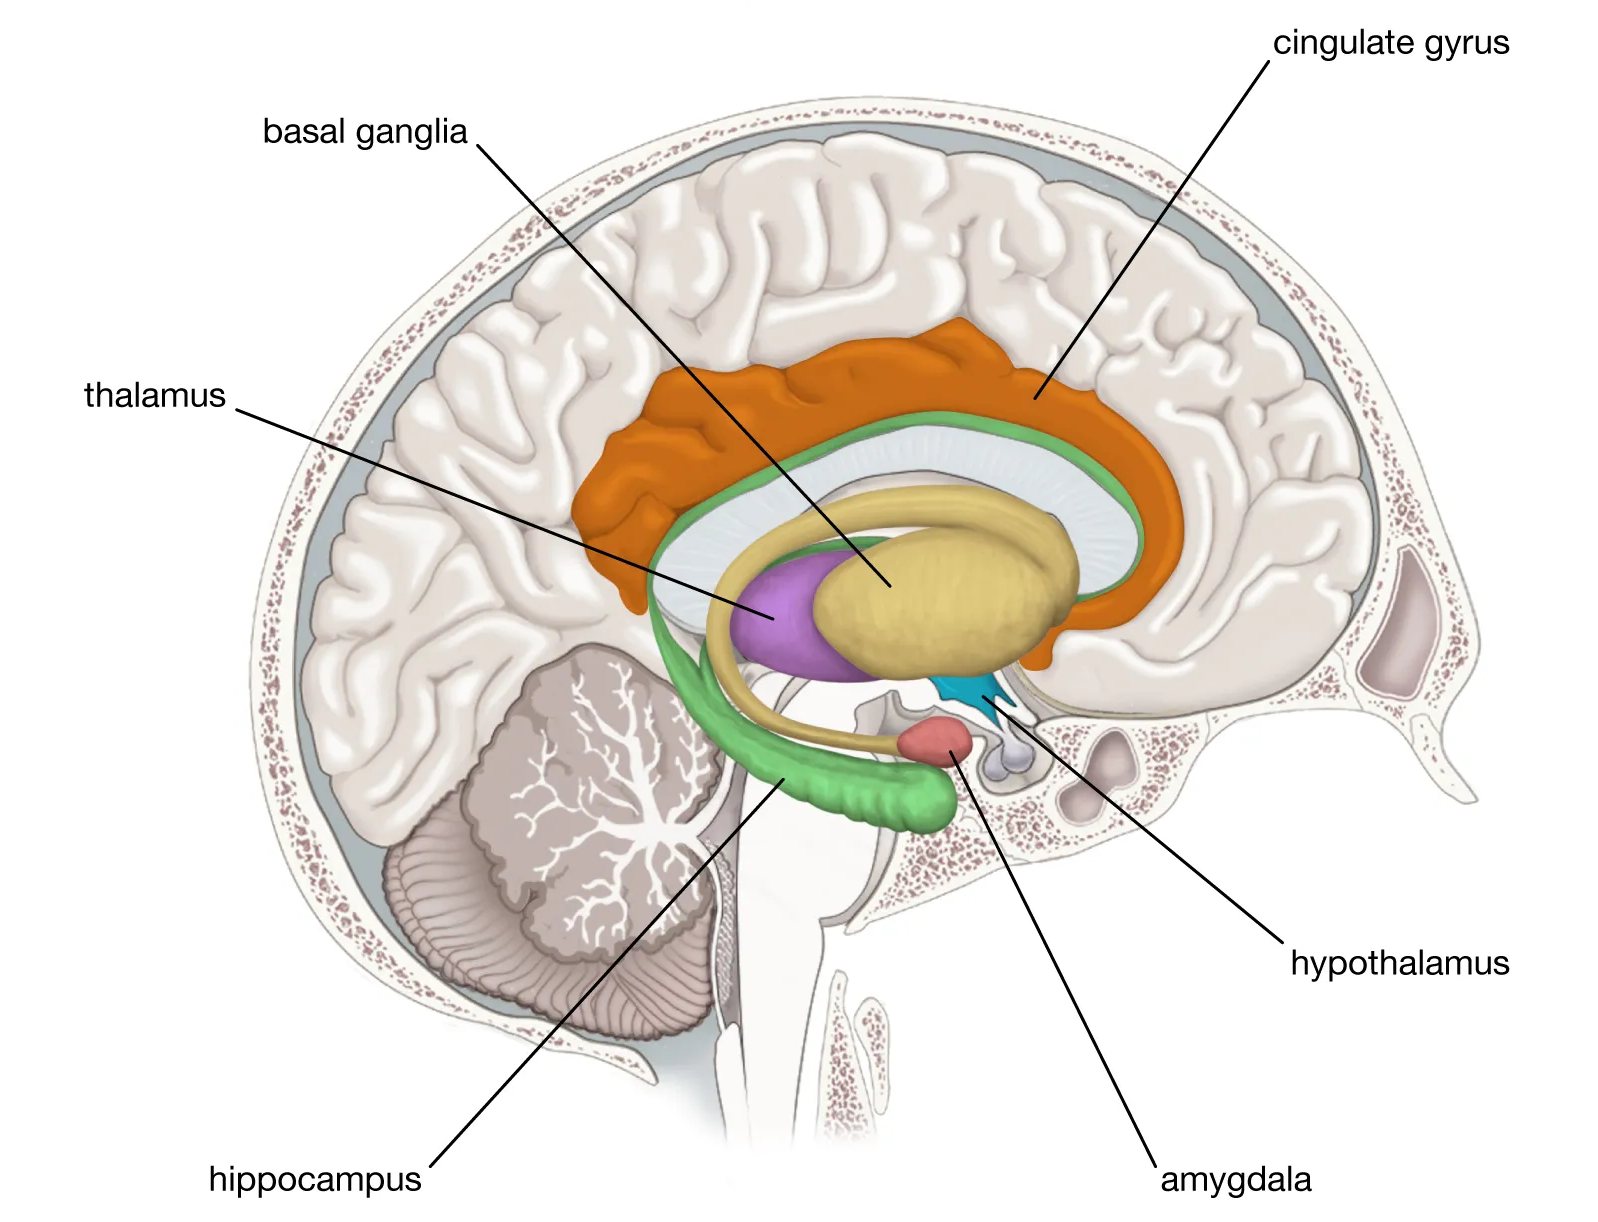
\includegraphics[width=0.5\linewidth]{images/brain-limbic-system-cut.png}
        \caption{Primary components of the limbic system (\cite{LimbicSystem} - modified)}
        \label{fig:limbic-system}
    \end{figure}

    Due to its high interconnectedness with other parts of the brain, there is no overall agreement on every component of the limbic system. Nonetheless, the structures depicted above can be considered its primary components. As a whole, it is involved in emotional responses, olfaction, and motivation but also the formation of long-term memory \cite{LimbicSystem}.

    % possible elaboration of more specific brain structures, that are related to the cognitive processes i am going to research

    Taking a look at the basic functionality of the brain and how it processes information, we encounter two very different aspects of its signal propagation. Whilst one is composed of direct and precise wiring between neurons, the other one is way more diffuse and based on a broader modulation of signals. \\
    The brain's wiring is established with the help of axons, which are an extension of a neuron that propagates a signal to its connected neurons. They enable fast and precise communication between various parts of the brain. Circuits that are formed like this, make complex processes possible and allow for essential information exchange. For example, our emotional limbic system and the rational cortex are connected like this and therefore can maintain a constant dialogue to integrate their desires \cite{thebrain-SimpleToComplex-neuroFunction-b}.

    %elaboration on hormonal brain?


\subsection{Neurons and Glial Cells}
%Cellular Organisation:
    % Neuron Anatomy
    The human nervous system allows us to respond to internal and external stimuli and comprises two types of cells. Neurons are the ones that transmit information with the help of electrical and chemical signals. Glial cells on the other hand act in a supportive manner. \\
    \textbf{Neurons} consist of the usual cell body but also show two additional parts: dendrites and an axon. Both play an important role in the transmission of information. Dendrites exhibit a tree-like structure, which is responsible for receiving input from other cells. The Axon is the extension of the cell that transports signals outwards. The length of these axons can vary by a lot. Whilst some only connect to other neurons in the brain and therefore are fairly short, others stimulate muscles over a long distance. But not only does the length of the axon differ between neurons. Depending on their role in the nervous system, they can take on many different shapes and sizes (Figure \ref{fig:neuron-types}) \cite{Banich.2018}.
    
    \begin{figure}[H]
        \centering
        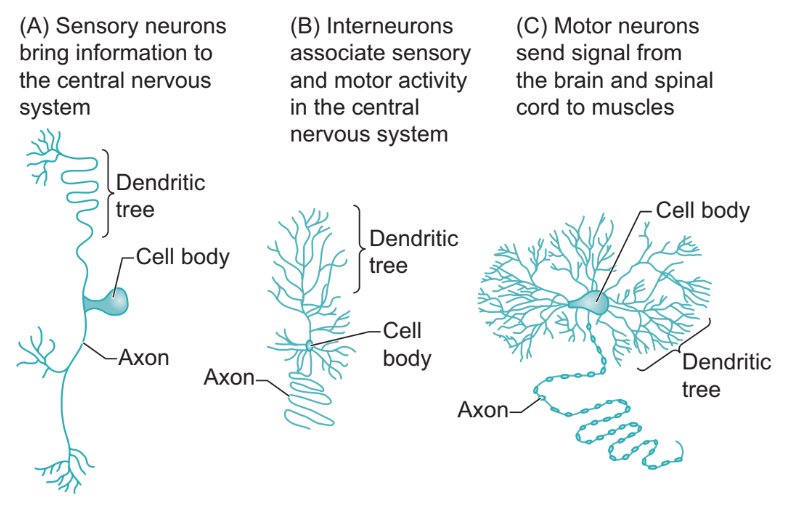
\includegraphics[width=0.75\linewidth]{images/neuron-types.png}
        \caption{Common examples of neurons \cite{Banich.2018}}
        \label{fig:neuron-types}
    \end{figure}

    
    % Glial Cells' anatomical role
    There exist different types of \textbf{Glial cells}, which all play an important role in intercellular communication. Even though their involvement might be a bit less obvious than that of neurons, they are just as essential for our nervous system. In fact, without them, the transmission of information via the neurons, would not even be possible \cite{Banich.2018}. 
        % Different types and their function, briefly mention role of axon myelination
        The following glial cells support the functioning of the central nervous system:
        \begin{description}
            \item[Astrocytes:] They take on the most complex functionalities of glial cells, which range from supplying mechanical support to maintaining and cleaning the extracellular environment \cite{thebrain-SimpleToComplex-cellularFunction-i}. But most importantly they provide neurons with nutrients. Via a connection to the capillaries in the Brain, they let glucose enter into their cell, partially metabolize it, and pass it on to the neurons \cite{thebrain-SimpleToComplex-cellularFunction-a}.
            \item[Microglial cells:] This type of glial cell acts protectively, as a primary defense mechanism against invaders. Therefore they can be considered the macrophages of the brain. 
            \item[Oligodendrocytes:] These cells provide a unique structural support, by wrapping around the axons of numerous neurons. Doing so in a very specific way, they create a myelin sheath that allows for accelerated conduction of nerve impulses \cite{thebrain-SimpleToComplex-cellularFunction-i}
        \end{description}

    
    % Neuronal Functions: specifics on how action potentials work
    Only when all these structures of different neurons and glial cells work together, can our brain function properly. Everything we experience, like thoughts, emotions, and the ability to move, is based on the capability of individual neurons to communicate.
    
        % Electrical properties, thresholds, place of summation and electrical conduction
        Taking a closer look at how this communication takes place, two complementary processes become apparent. One is the \textbf{chemical transmission} of signals which can be found between two neurons, at the synapse. Here chemical messenger molecules are transferred from the sending neuron to the receiving side. Details regarding this process will be covered in a later subsection dedicated to the synapse and molecular processes in the brain. \\
        When a signal arrives at another neuron, an electrical impulse arises. This impulse is then propagated inside the neuron via the other process, called \textbf{electrical conduction} \cite{thebrain-SimpleToComplex-cellularFunction-b}.
        % Relate to information value (all or nothing, frequency relevant)
        The dendrites of a single neuron receive impulses from thousands of other neurons. These impulses can either be excitatory (meaning they increase the probability of triggering a new impulse in the neuron) or inhibitory (when they reduce this probability). Depending on the type of impulse, a small potential is generated inside the neuron, which is positive for excitatory ones and negative otherwise. With the help of passive diffusion, this potential is propagated toward the cell body, losing intensity the further it travels. At the beginning of the axon, a summation of all impulses takes place. Only when the neuron's excitatory threshold is exceeded, a new impulse is generated and sent down the axon. In contrast to the passive diffusion, this so-called \textit{action potential} propagates actively with a maintained signal strength \cite{thebrain-SimpleToComplex-cellularFunction-i}. \\
        \textbf{Action potentials} are an "all or nothing" signal, meaning they do not vary in amplitude or intensity. Regardless of how far the neuron's threshold is exceeded, it will always result in the same signal. Therefore, a neuron can only transmit information by varying how many action potentials it generates per second. An action potential is propagated extremely fast and at any given point of the axon, it will not last longer than a few milliseconds. After it passes, the axon membrane exhibits a short refractory period, during which it cannot be stimulated. This also prevents the signal from being propagated in the wrong direction \cite{thebrain-SimpleToComplex-cellularFunction-a}

        % image action potential?
        
    % Myelination in detail
    To enable such a rapid propagation of the nerve impulses, many axons are wrapped inside an insulating sheath. This \textbf{myelin sheath} consists of a fatty substance and is formed with the assistance of glial cells. Within the brain, oligodendrocytes take on this task by wrapping their cell membrane around the axons.
        % nodes of Ranvier, place of ion channels
        But this sheath does not envelop the entire length of an axon, leaving gaps called \textit{nodes of Ranvier}. These nodes, spaced from 0.2 to 2 millimeters apart, facilitate a special conduction mechanism. Action potentials only have to leap from one node to the next, where the ion exchanges occur that regenerate the signal. In contrast to the continuous propagation of non-myelinated axons, this "saltatory conduction" is more efficient and much faster \cite{thebrain-SimpleToComplex-cellularFunction-i}.

 

\subsection{Synapses and Ion Channels}
%Molecular Organisation: 
    % Synaps Anatomy
    The place where an axon, connects to the dendrites of another neuron, is called a synapse. 
        % Electrical and Chemical
        Generally, there are two different types of synapses. One is the \textbf{electrical synapse}, where the cells touch physically and are connected by minuscule openings, that allow for a direct transmission of nerve impulses between them. Secondly, via \textbf{chemical synapses}, where the neurons remain separated and specific molecules have to traverse the gap to transmit the nerve impulse.
        While electrical synapses facilitate a swift transmission, chemical synapses are comparatively slower yet offer significantly more flexibility. This flexibility is fundamental to the process of learning \cite{thebrain-SimpleToComplex-mollecularAnatomy-b}. \\
        % Chemical Synaps in depth
        % Neurotransmitters (excitatory, inhibitory)
        The basic anatomical structure of such a chemical synapse can be seen in Figure \ref{fig:synapse} and facilitates the signal transmission as follows:
        % Function of Synaptic transmission (and role ion channels)
        When an action potential of the presynaptic neuron arrives at the terminal bouton (or axon terminal), the electrical signal is transformed into a chemical one. This happens with the help of synaptic vesicles, which contain neurotransmitters. These vesicles are waiting inside the terminal bouton and fuse with its membrane upon arrival of the action potential. Consequently, many molecules of neurotransmitters are released into the \textit{synaptic cleft}, which describes the gap between the pre- and postsynaptic neuron. When they reach the other side, they bind to receptors which are embedded into the membrane of the postsynaptic neuron. Receptors are proteins that change their configuration in response to the binding of a neurotransmitter and therefore the electrical charge of its neuron. They do so by influencing the ion flow across the membrane. Whether this results in an excitatory or inhibitory potential, depends on the receptor \cite{Banich.2018}.
        
        \begin{figure}[H]
            \centering
            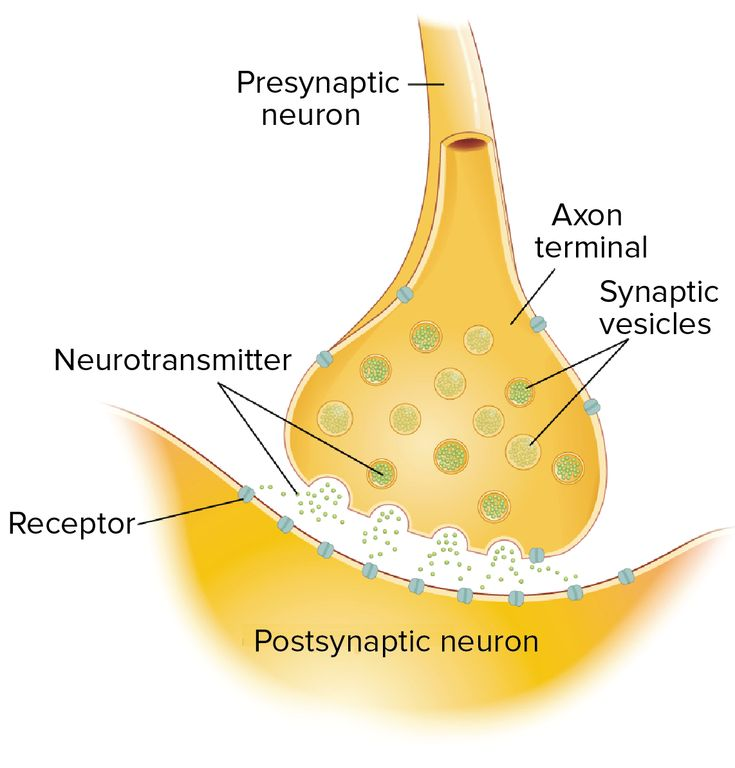
\includegraphics[width=0.5\linewidth]{images/synapse.jpg}
            \caption{Basic anatomy of chemical synapse}
            \label{fig:synapse}
        \end{figure}
        
    % Ion Channels and Nerve Conduction in Axon
    Any nerve impulse propagated inside our neurons, is simply the movement of electrically charged molecules (also known as ions) across the neural membrane. But without specialized \textbf{ion channels} in the membrane that coordinate this movement, something complex like our self-awareness would never be possible. Therefore, our brain relies heavily on these channels, consisting of large proteins. On a fundamental level, they give the neuron membrane a semi-permeable property, meaning that some ions may traverse it more easily than others. This semi-permeability controls, how the charged molecules distribute themselves across the membrane. In a resting state, an equilibrium is reached where the charge inside of the neuron is more negative than outside \cite{thebrain-SimpleToComplex-mollecularFunction-i}. %Resulting in a resting potential of about -70 millivolts.
    \\
    Should this equilibrium be disturbed and a strong enough depolarizing stimulus arise at the beginning of an axon, the ion channels are also responsible for \textit{producing the action potential}. By allowing many positively charged sodium ions to enter the cell, a strong depolarization happens and for a moment, the cell's charge even becomes more positive than outside. Then the channels of other positively charged potassium ions open, so they can leave the cell, and the ones of sodium close again. This leads to a strong hyperpolarization, such that the relative charge becomes even more negative than in the beginning. After the potassium channels close as well, the neuron slowly re-assumes its equilibrium and resting potential \cite{Banich.2018}.
    This sequence takes place at one node of Ranvier after the other, which is how the action potential is propagated to the end of the axon.
    


\section{Cognitive Processes}
    
    % Introduction to the General topic
        % What are coginitve processes
        % which ones am i presenting
    Cognitive processing refers to a series of activities involved in creating and managing mental representations of information. Cognitive processes encompass for example: attention, perception, reasoning, learning, but also the expression of emotions and more.
    They can occur consciously, such as when learning a concept, or unconsciously, as in skill acquisition. Further, they may be internally generated, like when recalling a memory or prompted by new sensory input from the environment, such as when navigating a maze \cite{Krch.2011}.
    % Create logical integration of section into thesis and a short overview
    % Specifically, the perception of emotions like fear and anxiety, are of special interest in the context of this thesis. Therefore, this section explores the involved cognitive processes, including the related brain structures and their neural topology. 
    
    \subsection{Emotions - Fear and Anxiety}
        % What is Fear and Anxiety
        % What is their function
        Fear and anxiety exist in the first place to alert us of potential dangers, threats, or conflicts and prompt us to respond appropriately. While some experts see fear and anxiety as the same thing, others believe they are different experiences \cite{Steimer.2002}.
        Even though they fall into the same category of alert signals, they arise in different scenarios. Whilst fear prepares us when confronted with a known external threat, anxiety takes over in case of internal conflict or when the danger is unknown \cite{kj.1995}.
        But also if anxiety and fear are considered different emotions, they can still share similar brain and behavior patterns. Some even suggest that anxiety could simply be a more complex version of fear, helping us to adapt and prepare for what is ahead \cite{Barlow.2000}.

    \subsubsection{Related Brain Structures}
        % what structures are involved (amygdala, simple circuit)
        % how does activity in amygdala relate to fear
        
        % 0. The biology of fear - 235, 238
        There are specific brain circuits involved, when we experience emotions and research has made good progress in the last decades to identify them \cite{Steimer.2002}. The long-established assumption, that emotions like fear and anxiety originate almost entirely from the limbic system, is by now considered obsolete \cite{LeDoux.2000}. 
        Nonetheless, the \textit{amygdala} (which is part of the limbic system) plays a central role, when it comes to fear and anxiety. 
        %(Using Neuroscience) -> amygdala damage
        It has for example been shown, that people with brain damage in the area of the amygdala, do not show physical reactions to threats \cite{Phelps.2006}. 
        % 1. The biology of fear 237 -> electrical stimulation = fear
        Other studies found that the electrical stimulation of the amygdala causes a complete fear response. Specifically, the lateral and central nuclei of the amygdala have been identified to generate the strongest responses and therefore may be considered the most important \cite{panksepp.1998}. \\
        % 2. The amigdala -> anxiety related to amigdala 2.0
        But many studies have also shown that for anxiety responses as well, the amygdala is of central importance \cite{Ferry.2017}. 
            % activity of amigdala = anxiety 2.2
        \textcite{Kim.2011} have suggested, that the activity level of the amygdala, may correlate with the intensity of anxiety - even if no threat was involved. \\
        As already suggested, it is not surprising that anxiety seems to be most dependent on sub-regions of the amygdala, that are similar to those related to fear. Next to the basolateral complex and the medial nucleus, the central nucleus appears critical \cite{McDonald.1982}. This central nucleus is, based on studies with rodents, crucial for the basic defensive responses, that are triggered by fear \cite{Davis.2001}.
        
        
    \subsubsection{Neural Topology and Molecular Mechanisms}
    
        % how are the Neurons connected there?
            % different structure of subnuclei - The Amygdala 2.1
            All the above-mentioned nuclei of the Amygdala, exhibit differences in their cell types, but also when it comes to connectivity and functional organization \cite{McDonald.1982}.
            % central nucleus essential
            Since the \textit{central nucleus} seems to be the part of the amygdala, that correlates the strongest with fear and anxiety, it would pose an interesting structure to simulate the cognitive process. 
            
        % what neurotransmitters are involved?
            Many neurotransmitters and other neuromodulators are involved in fear and anxiety \cite{Steimer.2002}. Amongst these, \textit{GABA} plays an important role. With its inhibitory function, it can help to calm the neuronal hyperactivity that is associated with anxiety \cite{thebrain-emotions-mollecular-a}.
        

    \subsection{Learning and Memory} 
    % Psychological
    % Very top-level definition of learning and Memory and how it works
    % differentiation short/long term memory - functionally
    Learning allows us to hold on to information, emotions, and impressions that can shape our behavior. It is the brain's primary function, wherein it constantly adapts its structure to better represent our experiences. This leads to memory, the lasting presence of personal experiences and general knowledge.
    Such memories are based on our perception of things and connect the information about different aspects, processed across our brain.\\
    Different forms of memory can be distinguished. \textit{Short-term memory} for example, allows for the retention of information for not more than a minute and is created based on what sensory inputs were paid attention to. An extension of this concept is the \textit{Working memory}, which facilitates cognitive operations on temporarily stored information, like reasoning, performing computations, or recalling a recently heard list.\\ 
    \textit{Long-term memory} on the other hand, describes any memory that is maintained over a longer period. It includes memories that are consolidated to different degrees and therefore can be recalled from days to years later \cite{thebrain-memory-psychological-a}.

    \subsubsection{Related Brain Structures}
    % Neurological
    % Focus on the Hippocampus and its role
    % importance of Short wave ripples and theta nested gamma oscillations
    Regarding short-term and working memory, the prefrontal cortex plays a fundamental role. It merges the information stored across other parts of the cortex and allows for its retrieval and reasoning \cite{thebrain-memory-neurological-a}. But also the hippocampus and certain activity patterns there, are involved in working memory. \textcite{Axmacher.2010} suggest that certain rhythms produced by the hippocampus can be associated with working memory performance. Specifically, the coupling of theta (4-8 Hz) and gamma (25-100Hz) rhythms (so-called \textit{theta-nested gamma oscillations} \cite{Aussel.2018}), seem to be of importance.\\
    However, especially for consolidating memories and their transition into longer-term memory, the hippocampus plays a crucial role. It is responsible for the formation of new associations between different areas of the cortex. For example, connecting the music heard with the faces seen at a party, to form a memory of it. Whether such associations then are reinforced until they turn into long-term memory, can depend on different factors. One important being their emotional relevance, which is evaluated in cooperation with other parts of the limbic system \cite{thebrain-memory-neurological-a}. Relevant patterns and associations, that were made during the day, are further strengthened via the occurrence of high-frequency oscillations during sleep. These particular oscillations, which are also called \textit{sharp wave ripples} (SWRs), mimic the patterns in a temporally compressed manner and therefore enhance synaptic plasticity and memory consolidation \cite{Girardeau.2011}. As a certain association strength is reached, the associations become encoded in the cortex and the hippocampus stops being involved \cite{thebrain-memory-neurological-a}.
    
    \subsubsection{Neural Topology and Molecular Mechanisms}
    % Cellular, Molecular
    % Focus on cells of Simulation (Acetylcholine?)
    The hippocampus proper is made up of three major sub-areas, called the CA1, CA2, and CA3. These in turn consist for the most part of pyramidal neurons. Input comes from the entorhinal cortex (EC) via the dentate gyrus (DG), is then processed in the hippocampus proper, and sent out from the CA1 to the subiculum \cite{thebrain-memory-Cellular-a}.
    
    % Insert graphic of hippocampus anatomy

    On a molecular level, learning is facilitated by Long-term potentiation, which is a mechanism that allows the strengthening of synapses. This is usually triggered by a short but high-frequency stimulation of the presynaptic neuron, which leads to a stronger (higher amplitude) response of the postsynaptic one. This change in amplitude appears due to a series of processes, including the creation and efficiency increase of certain ion channels at the postsynaptic neuron \cite{thebrain-memory-molecular-a}.

    
\section{Cognitive Warfare}

    % Why is it necessary to elaborate on the topic and how am I going to do this (what is the structure and content of this subsection)
    \textit{Cognitive warfare} is a term for an emerging form of warfare, which encompasses a broad field of practices \cite{Backes.2019} \cite{Claverie.2022} \cite{EADS.2023} \cite{MAKSYMENKO.2023} \cite{McCreight.2024} \cite{Miller.2023}. This section explores some of its definitions and suggests a way of categorizing them. Furthermore, the category that is relevant for this thesis, is identified and described in more detail before the general relevance of the topic is pointed out.


    \subsection{Categorization of Cognitive Warfare}

        % What is Cognitive warfare (broad definition, mention different ones)
            % ref: CW-russian threat, cognitive warfare ethical analysis, the cw concept
        A range of definitions for \textit{cognitive warfare} can be found in the literature, which describe varying scopes and aspects of it. \textcite{Claverie.2022} for example take a very general stance when they define cognitive warfare as "the art of using technological tools to alter the cognition of human targets" \cite{Claverie.2022}. This leaves both the method and exact effects on cognition open and therefore encapsulates most associations with the term.
        Other literature defines it more specifically as "altering through information means how a target population thinks, and through that, how they act" \cite{Backes.2019} or points out the involvement of "technologies capable of influencing or controlling cognitive functions and emotional states" \cite{EADS.2023}.
        
        % What Forms exist (focus on electro-magnetic attacks)
        These more specific definitions already characterize two major forms that can be identified. One is the more established one, covered by \textcite{Backes.2019}, where \textbf{information} and knowledge are the main focus. With the help of propaganda and disinformation, the beliefs of large populations are manipulated in the hope of influencing their choices and behavior. \\
        The other form is characterized by advanced \textbf{technologies} and their more fundamental influence on cognition and mind. Attacks performed with such technologies can be labeled as \textit{NeuroStrikes}, and employ for example so-called "Soft-Kill Radio Waves" which essentially are a form of EMR. They can cause significant cognitive damage and interfere with their targets' brain function \cite{EADS.2023}. This thesis focuses on the latter form of cognitive warfare.

        
    \subsection{NeuroStrikes and the Havana Syndrome}
    
        Since NeuroStrikes are the relevant form of cognitive warfare for this thesis, their effects and underlying technology shall be explored in more depth. In this context, the \textit{Havana Syndrome} serves as an important reference, as it is the best-documented collection of potential NeuroStrike incidents. 
        
        The \textbf{Havana Syndrome} describes a condition, that was coined by a collection of health incidents, which were distinct from any previously documented, neurological, or mental disorder \cite{Pavlin.2020} \cite{Bartholomew.2024}. It occurred first in Havana in 2016, when an individual who was assigned to the U.S. embassy, suddenly suffered from acute pain, coupled with a loud noise and cognitive impairments, followed by a range of long-term symptoms. Similar cases arose over the following years, while a closer investigation was not performed until 2020 when the National Academy of Sciences published an extensive report. Even though the assessment was difficult, due to a lack of complete and uniform clinical data, it was suggested that the most probable source for the symptoms was a form of NeuroStrike (directed, pulsed \textit{Radio Frequency} (RF) energy). Other potential mechanisms, like chemical or infectious agents, were deemed highly unlikely or in the case of psychological and social factors, could not explain the whole picture \cite{Pavlin.2020}. Even though it has to be stated that this topic is still debated and contradicting arguments exist \cite{Bartholomew.2024}, most literature on the technical form of cognitive warfare considers this syndrome to be related to it \cite{EADS.2023} \cite{McCreight.2022} \cite{McCreight.2024}.

        Based on that, pulsed RF EMR certainly represents a relevant form of NeuroStrikes, which could be responsible for the impairment of a series of cognitive processes. Its exact effects on the brain and how they could be mitigated are the subject of this work.
        

    \subsection{Relevance}
        % active developments
        Many countries and institutions are already applying cognitive warfare to such a degree, that its importance should not be underestimated \cite{Claverie.2022}. Whilst there are several reports of Russia, practicing cognitive warfare in its information-based form to influence elections \cite{Backes.2019} and during times of war \cite{MAKSYMENKO.2023}, there also exist incidents that are associated with NeuroStrikes (as described in the previous subsection). Furthermore, the Chinese communist party is reportedly investigating technologies related to these attacks \cite{McCreight.2024} and even has a dedicated military program in place to develop weapons for this purpose \cite{EADS.2023}.
        
        % passive threat
        But regardless of the intentional and active developments of such attacks, it has to be recognized that even neuroscience research performed with good intentions and health improvements in mind, may be misused for harmful military purposes \cite{McCreight.2024}. Consequently, the threat imposed by these technologies and cognitive warfare of this form is already very real and will only become larger over time and with advancing research.



\section{Brain-Computer Interfaces}
    % General description of what brain interfaces are: gateway between brain and computer
        % reading brain signals (Nicolas)
        % stimulating brain (William)
        % Uni and Bidirectional (Rao.2019)
    Brain-Computer Interfaces are systems, that enable information transfer between the brain and a Computer. This encompasses technologies that allow for the sensing and interpretation of brain activity \cite{NicolasAlonso.2012}, as well as ones that enable neural stimulation \cite{WilliamJ.Tyler.2017}. These two technologies may also be combined to create a bidirectional system \cite{Rao.2019}.\\
    BCIs enable users to engage with their environment independently of peripheral nerves and muscles. They create a novel pathway, that translates their intentions into signals, which may control many devices like computers or prostheses. This enables for example people who are "locked in" or severely disabled, to communicate or regain other fundamental capabilities. It therefore is of especially high interest to those groups. However, BCIs also have potential use cases in non-medical environments like entertainment \cite{NicolasAlonso.2012}.
    
    % general sensing methods
    When measuring brain activity, for example, to interpret the users' intentions, there are generally two phenomena that can be observed. One is the \textit{electrophysiological} activity of the brain and the other consists of its \textit{hemodynamics} \cite{NicolasAlonso.2012}. \\
    The \textbf{electrophysiological} activity stems from the currents that arise during the propagation of action potentials and therefore is directly related to information processing \cite{Baillet.2001}.
    \textbf{Hemodynamic} changes, on the other hand, can be traced back to the fact that active neurons are supplied with more glucose and oxygen than inactive neurons. This leads to more oxyhemoglobin in the active areas and allows for a distinction from nonactive ones by observing the local oxyhemoglobin to deoxyhemoglobin ratios \cite{Laureys.2014}. This therefore is only indirectly related to the processing of information.
    
    % Invasive - non Invasive (8 reasons, WilliamJ)
    Many different detection and stimulation methods are used in BCIs, which may be categorized according to their level of invasiveness \cite{Bernal.2023}. In the following section, the differences between the two, as well as some specific examples are discussed.
        

    \subsection{Non-Invasive Brain Interfaces}
        Non-invasive methods have the inherent benefit of being applicable without prior surgery. Instead of implanting an electrode into the user's brain, they act outside of the skull \cite{WilliamJ.Tyler.2017}. Even though this means that they are limited to recording activity with lower resolution \cite{Lebedev.2006}, they certainly are the preferred choice for short-term usage scenarios \cite{Luan.2014}. \\
        % Measuring brain activity -> brain computer interfaces, a review
        The following are examples of such non-invasive methods.
        
        \subsubsection{Recording Methods}
        \begin{description}
            \item[Electroencephalography (EEG)] is a method that records the electrophysiological activity, being especially sensitive to the extracellular currents that come with it \cite{Baillet.2001}. Since it only requires electrodes to be placed on the scalp for measurements, it is a very easy and popular method. However, a major downside is the poor signal quality, which suffers from a lot of background noise.
            \item[Functional Magnetic Resonance Imaging (fMRI)] detects hemodynamic changes, like local blood volumes and flows, as well as oxygenation levels. It does so with the help of MRI scanners that create electromagnetic fields. This results in spaciously very accurate readings, that can be used to identify precisely which brain regions are active \cite{deCharms.2004}.
        \end{description}

        % Stimulating brain -> WilliamJ.Tyler.2017
        \subsubsection{Stimulation Methods}
        \begin{description}
            \item[Transcutaneous Electrical Neurostimulation (TENS)] is the broadest category of methods, to stimulate the brain non-invasively. The basic procedure constitutes the transmission of electrical current (which can be static or dynamic), via electrodes that are placed on the skin, to nerves. The applied current then modulates neuronal activity directly. Even though it is a complicated procedure to control which neurons are activated, this method can be very effective. It might even be possible to achieve drug-like outcomes with reduced side effects or augmenting cognitive performance \cite{WilliamJ.Tyler.2017}. 
            \item[Ultrasonic Neuromodulation (UNMOD)] is a unique method, which has been shown to allow, if applied in a pulsed manner, to stimulate neuron activity. Interestingly, it may do so via mechanical mechanisms of certain ion channels instead of influencing the electric charge directly \cite{Tyler.2008}. But the field of this methodology is still somewhat new and it will take time to create a deeper understanding of the mechanical influences on our brain activity. Nonetheless, it holds loads of potential for future development \cite{WilliamJ.Tyler.2017}.
        \end{description}


    \subsection{Invasive Brain Interfaces}
        % benefits compared to Non invasive
        Even though non-invasive interfaces are a great choice for many applications, there are scenarios where their limited precision is insufficient. For example, most researchers agree that without invasive methods, exercising control with multiple degrees of freedom over prostheses is impossible \cite{Lebedev.2006}. However as these invasive methods require the implantation of electrodes inside the skull, their application bears substantial health risks, that have to be addressed to make them a viable option \cite{Kennedy.2000}. \\
        % Measuring -> brain-computer interfaces, a review
        Some examples of such invasive methods are presented below.

        \subsubsection{Recording Methods}
        \begin{description}
            \item[Electrocorticography (ECoG)] is a method, where electrodes are placed on the brain surface, to record its electrical activity. It, therefore, follows a similar approach to EEG whilst being closer to the activity and avoiding the skull as an obstacle. Consequently, it achieves a higher spatial and temporal measurement resolution and is less susceptible to noise \cite{Ball.2009}. Advanced versions of this method, make it already possible for their users to control a cursor in two dimensions \cite{Schalk.2007}.
            \item[Intracortical Neuron Recording] is a technique, where electrodes are not placed outside, but rather inside the brain. Specifically into the cortex, where it measures the electrophysiological activity of neurons \cite{NicolasAlonso.2012}. Besides achieving a significantly higher resolution than non-invasive alternatives and providing easier-to-interpret signals, their quality can degrade over time. This can happen due to issues with cerebral tissue reacting to the electrodes \cite{Polikov.2005}.
        \end{description}
        % Stimulating
            % DBS (deep brain stimulations) -> 8 reasons
        \subsubsection{Stimulation Methods}
        \begin{description}
            \item[Intracortical Microstimulation (ICMS)] is a technique, that focuses on the stimulation of the cortex \cite{Vidal.2016}. It has demonstrated significant utility in comprehending the functions of cortical activity and enables the manipulation of sensory perceptions through brain stimulation. This simulation of sensory input has the potential to restore functional vision \cite{Zhao.2023} and could also be used to supplement prostheses with tactile perception and thereby improve the performance with it \cite{Flesher.2021}.
            \item[Deep Brain Stimulation (DBS)] is a method that comprises the stimulation of structures, that lie deep inside the brain and has been applied since the late 20th century. It delivers continuous stimuli, which can be adjusted in frequency and amplitude. This turned out to be useful for many different pathological situations, where it for example is applied to treat Parkinson's disease \cite{Benabid.2003}.
        \end{description}


    \subsection{Safety and Security}
    % Connection to previous BCI part (a lot of technologies that can be used in many beneficial ways...)
        % With increasing employment come also risks
            % Cyberattacks
                    % Information cycle -> Security in BCI's ?
    As presented above, there exist many different methods and technologies in the field of BCIs, which allow for a broad field of applications. And even though, the field is maturing \cite{Summerer.2009} and gaining a lot of popularity \cite{Bernal.2023}, there is not much work regarding the context of safety and security \cite{Brocal.2023}. However, BCIs bare the potential to be both, a source of risk \cite{Bernal.2021}, and a technology for risk prevention \cite{Liu.2015}. In the following, some examples of this will be discussed, before the role of BCIs in the context of this thesis is specified. 

    As \textcite{Bernal.2023} have shown, cyberattacks are an important example, of how BCIs can be a source of risk, by exploiting vulnerabilities of the technology. They pose the threat of private user information being stolen, or even the neural activity of the user manipulated \cite{Backes.2019}. Very alarming are therefore the findings by \textcite{Bernal.2021}, who analyzed and evaluated a large variety of attacks on different aspects of BCI technology. They found that even basic attacks may have a considerable impact on the safety of the user, which is especially problematic in the context that security measures for BCIs are still immature.\\
    % but they can also be used to grant safety
        % Risk identification
        % fatique detection
        % and potentially as protective measures against attacks
            % to be evaluated
    But as a collection of work shows, there also exist different approaches employing the technology of BCIs to reduce risks and improve the user's safety. This can for example be achieved by fatigue detection, which has been especially well explored \cite{Backes.2019}. As the mental state and fatigue have a significant impact on driving safety, systems like the one proposed by \textcite{Liu.2015}, can help to identify and avoid problematic conditions of the user during driving tasks.
    
    Mitigation technologies, like the ones explored in this work, may also qualify as a form of risk-reducing application. However, it is the subject of this research to show, how suited BCIs are to protect their users from the impact of electromagnetic attacks and how a protective system may be realized.
    

\section{Brain Simulations}
    Since the research of this thesis is in large parts performed with the help of simulations, this section provides an overview of the field. First elaborating on the topic and its importance in general, followed by some examples of Brain simulators.
    
    % 738 - Limited knowledge of brain
        % 741 - Until we learn
    We currently do not have a thorough understanding or an accepted theory on how the brain works on a large scale \cite{Einevoll.2019}. Even though experiments, trying to map a stimulus to its related brain activity, have been performed for quite some time \cite{Hubel.1959}, many principles of its operation remain unknown.
    % Simulations are a way to understand (even possible without?)
        % 735- still in infancy
        % 735 - cubic mil thousands of neurons
            % 736 - similar complexity as weather forecast
        % 736 - supercomputers as potential solution
    Brain simulations could help, or may even be necessary, to achieve an understanding of the wide range of mechanisms that are involved. It has to be recognized though, that the modeling of neural networks on a biological basis, is not yet a mature science. Especially due to the fact, that even representations of very small brain areas include thousands of neurons, such simulations were until recently, infeasible to compute. Although, with recent supercomputers, such limitations could be alleviated.
    % definitions:
    But before more details regarding such simulations are presented, a few terms shall be defined. Specifically, it is important to differentiate a \textit{Simulator} from a \textit{Model}. Whilst the \textit{Simulator}, describes a software tool that facilitates simulations, the \textit{Model} describes one specific collection of equations and parameters, that can be executed by such a tool (resulting in a \textit{Simulation}) \cite{Einevoll.2019}.\\
    % 739 - Models as hypothesis
        % 736 - various pros cons
    % 739 - Simulator to test hypothesis
        % Simulators usable without knowledge of every detail
    In this context, a \textit{Model} can therefore be considered as a hypothesis, of how the represented network structure might work. And with the help of a \textit{simulator}, it is therefore possible to test the hypothesis by comparing the outputs to the results of experimental findings \cite{Einevoll.2019}.\\
    In the following, a selection of simulators are presented, that are of interest for this work. An overview of potential models is then presented in the next chapter. 
        
    
    \subsection{Brian2}
    Brian2 is a simulator that works with mathematical abstractions. It allows the simulation of spiking neural networks, in an easy and efficient way, whilst maintaining a high level of flexibility. This is partly achieved, by basing its neuron models only on a set of mathematical equations. It thereby grants its users a large degree of freedom and enables them to investigate novel mechanisms without requiring a complex implementation in a low-level programming language. To increase the flexibility of the simulation process even further, it is written as a Python \cite{van1995python} library. Effectively integrating the benefits of a general-purpose programming language in the simulation environment. To still ensure fast processing of the simulation code, Brian2 makes use of runtime code generation, which transforms the simpler high-level statements, into efficient low-level code \cite{Stimberg.20.8.2019}.
    
    
    \subsection{NEURON}
    In contrary to Brain2, the NEURON simulator makes use of biologically accurate neuron models, emphasizing the realism of chemical and electrical signal transmissions, inside and across neurons. But whilst enabling the use of incredibly detailed models, the simulator leaves the choice of detail that is represented, to the creator of the model. However, it performs best in the realm of rather small and detailed networks, investigating low-level aspects like ion concentrations or membrane channel properties. It supplies a graphical interface that increases the simulator's usability, by enabling the adjustment of parameters and allowing for the representation of graphs. To investigate novel mechanisms, it provides its domain-specific modeling language NMODL, which for performance reasons is then automatically translated into C \cite{Hines.1997}. 

    
    \subsection{NEST}
    The NEST simulator employs simplified representations of neurons, that comprise few compartments at most. Therefore it is more directed toward the simulation and investigation of larger networks, instead of single neuron properties. It supplies a flexible simulation environment, that can be used with different user interfaces, including a module for Python and also a proprietary simulation language called SLI. New mechanisms can easily be added, thanks to its modular architecture, which not only allows the addition of novel neuron models but also enables the creation of simulator functions and even extensions to the simulation language itself. Regarding performance, NEST can leverage multiprocessors and computer clusters to achieve a higher simulation speed and increase memory capacity \cite{Gewaltig:NEST}.

\chapter{Related Work} % application of concepts
\label{chap:related-work}

% Try to highlight the differences between the state-of-the-art and your thesis. The goal is to:
% (a) do not re-invent the wheel, we can use major pillars of existing work to build upon
% (b) similarly, we do not want to propose something that is already existing. Thus, we need to show the "delta".

% not really any similar work available, therefore considering a larger scope and show the basis for my experimental setup:
As the whole field of NeuroStrike research and brain-computer interface simulations is very novel, there unfortunately does not exist any directly related work. To the best of our knowledge, no research regarding simulations of NeuroStrikes and potential mitigation approaches has been published. Therefore the scope of analysis for related work was expanded. \\
By following this approach, relevant literature could nonetheless be identified, and important findings and approaches derived. Especially previous work that is related to the simulation character of this research, was considered.\\
First, some \textit{models for the simulation of cognitive processes} were analyzed and compared, to ensure the relevance of later performed research on top of such a model. After that, the extended literature related to the \textit{simulation of NeuroStrikes} was considered. 


\section{Models for the Simulation of Cognitive Processes}
% as concise as possible, documentation of the models I compare
    In the first step, it is essential to choose a suitable Model for the simulation of a cognitive process. For a model to be suitable in the context of this work, it has to adhere to some key criteria, specifically:
    \begin{enumerate}
        \item It has to represent a brain area, that is \textbf{related} to a cognitive process and affected by NeuroStrike attacks.
        %(The Amygdala or Hippocampus and their associated processes of fear/anxiety respectively memory/learning are of special interest, as they are best related to the effects of NeuroStrikes (reference?)).
        \item It has to allow for the simulation of the cognitive process in a \textbf{meaningful} and measurable way.
        \item The model and its associated simulator have to facilitate the \textbf{integration} of the attack and its countermeasure into the simulation.
        \item It should be as \textbf{realistic} as possible.
    \end{enumerate}

    Based on the literature presented in the previous sections and the first criteria, the search for potential models was directed towards ones of the hippocampus and amygdala. Furthermore, the "NEST" \cite{Gewaltig:NEST}, "NEURON" \cite{Hines.1997}, and "Brian2" \cite{Stimberg.20.8.2019} simulators (introduced above), were deemed to be the most suitable options for the given research conditions, which also guided the preliminary selection. The search for potential models was conducted on ModelDB \cite{McDougal.2017} and the most promising ones identified there are followingly analyzed in depth and compared in the end.

    \subsection{A 1000 cell network model for Lateral Amygdala}
    % https://modeldb.science/150288
    This model represents the dorsal part of the lateral amygdala (LA) and was written for the NEURON simulator. It was created to assess the importance of different factors that play a part in fear conditioning. The evaluated factors were: the increased responsiveness of neurons projecting to the LA, their synapses' plasticity, and LA internal synapses' plasticity. To monitor their effect on fear conditioning, they observed the temporal pattern of the neurons increase in tone responsiveness \cite{Kim.2013}, which is associated with fear conditioning \cite{Repa.2001}. \\
    It is a bio-physically realistic model which is scaled down in a ratio of 30:1. Therefore consisting of 1'000 neurons (800 principal cells and 200 interneurons), which are connected by almost 40'000 synapses. The neurons were modeled with multiple compartments (cell body and one or two dendrites) and different spiking frequencies (for the principal cells). Due to the high number of neurons, they were distributed randomly in a 3-dimensional space and connected based on some observed general rules and their derived probabilities. On average resulting in about 60 excitatory and 20 inhibitory inputs per principal cell. Component-wise adjustments were impossible for the model tuning and validation process, due to its scale. Nonetheless, it managed to reproduce the expected high-level behavior precisely, even though it is mostly based on low-level details. \\
    Regarding the input, the model incorporates the simulation of thalamic and cortical inputs via glutamatergic synapses acting on AMPA/NMDA receptors (at 20 or 40 Hz). But also random excitatory background inputs to all model cells \cite{Kim.2013}.

    \subsection{Model of CA1 activity during working memory task}
    % https://modeldb.science/223962
    This is a model that represents some neurons of the hippocampus, specifically pyramidal cells from the CA1 region. It was also written for the NEURON simulator and created to investigate working memory capacity (WMC) on the single neuron level. The WMC was analyzed in the context of a delayed free recall task, where a certain amount of items from a list must be recalled. To quantify the performance, the cumulative latency of this free recall was taken as a benchmark. Lower latency values are associated with higher WMC, whereas higher values suggest the opposite. \\
    The simplifying assumption was made, that a single neuron of the hippocampus could code for an object and would fire if it was presented with the according stimuli of the sensory systems. On a structural level, that meant that each neuron was modeled the same, with 26 oblique dendrites, originating from the cell body. Each dendrite conceptually represents a feature, which allows the neuron to encode for objects, by responding to certain combinations of these. During the simulation, random groups of 1 to 26 dendrites were then stimulated with synaptic inputs, while a level of realistic background synaptic activity was maintained. This background activity balanced to achieve an average resting potential of -65 mV. The number of neurons simulated was matched to the number of words that should be recalled, resulting in the simultaneous simulation of 6, 9, or 12 neurons. \\
    The main adjustable parameters of the model are the amount of dendrites that are being stimulated, as well as the level of background noise. The dendritic location of the synapses, as well as the pattern of background activity, was randomized across simulations \cite{Spera.2016}.
    
    
    \subsection{Model of the hippocampus over the sleep-wake cycle using Hodgkin-Huxley neurons}
    % https://modeldb.science/243350
    This is a detailed model, which represents the hippocampus as well as the entorhinal cortex in an anatomically accurate fashion. It was written for the Brian2 simulator in Python to analyze the effects of different changes in the network that appear during the sleep-wake cycle. Especially the role of varying acetylcholine concentrations during these cycles was explored, by simulating their modulatory effect on the functional connectivity of the hippocampus. To quantify the results, the output (in the form of extracellular recordings) was analyzed and compared to the expected oscillatory rhythms. \\
    Each neuron was simulated according to Hodgkin-Huxley's model as single-compartment and conductance-based. Principal excitatory neurons were modeled as pyramidal cells with sodium, potassium, and calcium ion channels. Some of them also received a Calcium-Activated-Nonspecific (CAN) cationic channel. Interactions between neurons were modeled with excitatory and inhibitory synapses. In total over 30'000 neurons were used to represent the hippocampal formation and entorhinal cortex. The hippocampal formation was further divided into the "dentate gyrus", CA1, and CA3, where the amount and type of neurons in each structure were adjusted to match values suggested by the literature. But also the whole spatial organization was matched to the human anatomy as shown in Figure \ref{fig:hippocampus-model}. The importance and benefits of this have been shown by \textcite{Aussel.2018}, who compared its performance against less realistic topologies and connectivity settings.
    \begin{figure}[H]
        \centering
        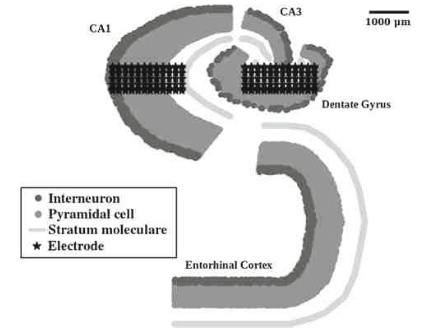
\includegraphics[width=0.45\linewidth]{images/hippo-model-brian2.png}
        \caption{Topology of the Model \cite{Aussel.2018}}
        \label{fig:hippocampus-model}
    \end{figure}
    The external input is only inserted at the neurons of the entorhinal cortex and then propagated to the other structures from there. To represent inputs from the rest of the brain as realistic as possible, each input neuron is stimulated by a variable firing rate, derived from real recordings of sleep/wake SEEG signals. Furthermore, the model offers many conductance-related and general parameters that can be adjusted \cite{Aussel.2018}. 
    

    \subsection{Comparison and Conclusion}
    % Show table of compared models and mention and justify the selected model based on information supplied
    Considering these models under the criteria mentioned at the beginning of the section, the \textit{model of the hippocampus} turned out to be most suited for use in this thesis.\\
    Whilst the model of the \textit{lateral amygdala} did not allow for a strong enough relation to the performance of a high-level cognitive process, the one concerned with \textit{working memory capacity} lacks the necessary realism. Even though every neuron is modeled realistically, its limited network size makes inferences on complex cognitive processes difficult.\\
    The model of the \textit{hippocampus} on the other hand, adheres fairly well to all the criteria. It provides a clear and measurable relationship to learning and memory, by observing certain activity patterns. Furthermore, it supplies a large parameter space, which should facilitate the integration of the electromagnetic attack. Lastly, modeling as many neurons as it does, in a spatially accurate manner, makes it the network-wise most realistic option.
    


\section{Simulation of Neurostrikes}
% What work has been done, regarding the Attacks
    To simulate the impact of neurostrike on the brain, their exact effects on the brain need to be explored and understood. This section therefore is dedicated to assessing the state of the art when it comes to the simulation of such attacks and their underlying mechanisms. But as the whole topic of neurostrikes is novel and to a certain degree still disputed, not much literature can be found regarding its mechanisms and effects. Let alone any work of attack simulations in functional brain simulations. Therefore, this section is concerned with summarizing and discussing, what has been proposed by the current literature on neurostrikes. Filling the gaps where necessary with findings in the field of electromagnetic radiation, as it is considered the underlying technology. This shall then serve as a basis for integrating such an attack into the simulation and ultimately guide the design of a countermeasure.

    
    \subsection{Neurostrikes}
    % Based on what I simulate the attacks (NeuroStrikes) - specific effects of NeuroStrikes on the Brain (and area of the cognitive process)
    To ensure that the relation between the attack and cognitive warfare is maintained as well as possible, the available specific literature (even though sparse) will set the general frame for its implementation. Therefore the \textit{Havana Syndrome}, being the best-documented case of its potential occurrence and effects, will be analyzed first. The focus is set on the related symptoms as more specific elaborations are difficult without making assumptions about its underlying mechanism (which shall be reserved for the subsequent section).
    
    The symptoms that were reported in cases of the Havana syndrome, can be split into ones that occurred during the \textit{initial} and sudden onset of the illness, as well as \textit{persisting} or recurring ones.\\
    The \textbf{initial} symptoms were reported to mostly start with the perception of a loud sound, described as clicking or screeching, accompanied by a strong feeling of vibration or pressure and pain in the head. Interestingly most victims described these sensations to come from a specific direction. Less often were the reports of tinnitus, hearing loss, dizziness, unsteady gait, or visual disturbances.\\
    The \textbf{persisting} or long-term effects include some similar symptoms, but for the most part, are distinct. Dizziness for example is something that persisted in many individuals, but also headaches became chronic in some patients. Further reported symptoms include: fatigue, impaired balance, concentration, and memory, but also depression and insomnia \cite{Pavlin.2020}.
    

    \subsection{Electromagnetic Radiation}
    % since only little literature is available; supplement with research regarding "pulsed RadioFrequency Electromagnetic waves" and their effects
    To the best of our knowledge, also no previous work exists on simulating Electromagnetic attacks or EMR in general, inside a functional model of the brain or any substructure. Therefore, this section will discuss general findings and proposals, for the effects of EMR on the brain. A special focus will be laid on the supposed underlying technology of NeuroStrikes, pulsed RF EMR. But also general findings regarding EMR will be included to supplement the sparse literature. It should be mentioned that most of these findings were made through animal experiments and that the results are by no means uniform.

    % 1. electromagnetic radiation has effects on brain
        % Many studies indicate effect: Zhi.2017
        % Treshold intensity: DAndrea.1999
        A large body of literature suggests that EMR can have a series of negative effects on the brain and its function \cite{Hu.2021} \cite{Lai.1994} \cite{Zhi.2017}. However, the specific effects on the brain can differ, depending on a few radiation exposure parameters. For example, it may require a certain irradiation intensity threshold to be reached, before significant changes appear at all \cite{DAndrea.1999}. Whilst for RF radiation, their modulation into pulses seems to be essential \cite{Huber.2005}. But also the radiation frequency in general and its power plays an important role, as changes in these parameters can lead to alterations of the observable effects \cite{Hu.2021}.
        
    % 2. changes of activity, damage to brain areas, neurotransmitter changes
        % General: Tan.2017
        % Highlevel effects: Anxiety - Kereya.2018, Headache/memory - Lin.2021
        % Neurotransmitter changes: Acetylcholine increase - Kumar.2016
        From a \textbf{high-level} (functional) perspective, \textbf{effects} include the emergence of fear or anxiety \cite{Kereya.2018}, but also impairments of learning, memory, headaches, and more \cite{calvente2016does} \cite{Lin.2021} \cite{Tan.2017}. This is similar to the functional impairments that are associated with NeuroStrikes. Specifically considering the reports related to the Havana syndrome, as presented above.\\
        Regarding \textbf{lower-level effects} of EMR and potential causes of these functional impairments, different alterations in the brain have been observed. However, the focus was set according to the simulation model choice and directed towards the hippocampus and memory impairments.\\ % Insert more details if necessary
        One category of identified alterations was \textit{structural damage} to certain brain areas \cite{Hu.2021} \cite{Tan.2017}, for example, the hippocampus and cerebral cortex \cite{Lin.2021}.\\
        Furthermore, a wide range of \textit{neurotransmitter changes} were recorded in the context of EMR. Including alterations in dopamine, serotonin, norepinephrine, and acetylcholine levels \cite{Hu.2021}.\\
        But changes in general \textit{electrophysiological activity} have also been reported, specifically after exposure to RF EMR. Some experiments for example showed that the majority of irradiated cells reduce their spontaneous activity \cite{seaman1978slow} \cite{wachtel1975effects}. Others identified differences between initial and long-term effects, where the excitability of the neurons is increased in the beginning and only reduced after longer exposures \cite{dumansky1974biologic}.

    % 3. radio frequency effect on hippocampus and amygdala
        % General: Lai.1994, Narayanan.2019
    
    \subsection{Conclusion and derived parameters}
    The literature supplies a lot of indications that NeuroStrikes and specifically RF EMR, do impair the cognitive processes of memory and learning. A few underlying changes could further be identified to be the most promising cause for that. First of all, the structural damage to the hippocampus, as this structure plays an important role in the cognitive process. But also changes in the neurotransmitter acetylcholine could be responsible for the disturbance of those processes, as they play a key role in their modulation \cite{Aussel.2018}.
    

\section{Research Gap and Motivation}
% Clear identification of Knowledge gap in the literature 
    % -> Underlying Mechanisms of Neurostrikes
    % show with table
To conclude the review of related work, that was performed in this chapter, an overview of the available literature will be performed in this section. This shall summarize what has been done, and allow for a clear identification of the research gap. In the following, the available resources and literature on the simulation of cognitive processes are evaluated, before a more detailed analysis is performed on the works related to NeuroStrikes.

    \subsection{Simulation of Cognitive Processes}
    In the realm of brain simulators and works that are related to them, it was possible to identify a series of resources that fulfill the general requirements for this work. Showing that there exist simulation models, that combine a realistic topology with the capability to represent the performance of a cognitive process. As specified in the according section, some of the investigated models, are better suited than others. Especially because such complex models, incorporate many aspects, that need to fit the specific use case. The available resources do however cover the simulation field of interest sufficiently, which allows this work to focus its research on other aspects. 
    

    \subsection{Simulation of NeuroStrikes}
    A goal of this work is, to integrate a NeuroStrike (or Electromagnetic attack) into the simulation of the cognitive process. As however already discussed in the dedicated chapter above, the literature on NeuroStrikes is sparse. Especially regarding any specific explorations of their effect on the brain. It is, therefore, no surprise that even less literature, respectively none at all, could be identified, that integrates such an attack into a simulation. The alternative approach, investigating the most probable underlying technology of NeuroStrikes (RF EMR), has also been elaborated in more detail.

    \begin{table}[htbp]
        \centering
        \caption{Overview of existing work on NeuroStrikes and their mechanism}
        \begin{tabular}{@{}m{3cm} m{2.5cm} m{4cm} m{5cm}@{}}
            \toprule
            \textbf{Context} & \textbf{Reference} & \textbf{Investigated Aspects} & \textbf{Findings} \\ 
            \midrule
        \end{tabular}
        \renewcommand{\arraystretch}{1.3}
        \begin{tabular}{@{}p{2.9cm} p{2.5cm} p{4cm} p{5cm}@{}}
            NeuroStrikes 
                & \small{\textcite{McCreight.2024}} & \small{general assessment} & \small{high relevance, related to nano pulsed RF EMR} \\
                & \small{\textcite{EADS.2023}} & \small{general assessment} & \small{high relevance, causes cognitive impairments through \newline series of technologies} \\ 
                & \small{\textcite{McCreight.2022}} & \small{symptoms and potential causes} & \small{many symptoms, caused by RF EMR} \\
                & \small{\textcite{Pavlin.2020}} & \small{symptoms, potential causes, and brain \newline alterations} & \small{wide range of acute and persistent symptoms, likely caused by RF EMR, showing unspecific brain damage} \\ 
        \midrule
            Electromagnetic Radiation
                & \small{\textcite{Narayanan.2019}} & \small{symptoms} & \small{can cause range of symptoms} \\
                & \small{\textcite{Zhi.2017}} & \small{symptoms and brain \newline alterations} & \small{many mechanisms involved in cognitive impairments} \\ 
                & \small{\textcite{Tan.2017}} & \small{symptoms and brain \newline alterations} & \small{many mechanisms lead to memory impairments} \\ 
                & \small{\textcite{Lai.1994}} & \small{brain alterations} & \small{overview of many effects on the brain} \\
                & \small{\textcite{Lin.2021}} & \small{brain alterations} & \small{neurotransmitter changes and damage in hippocampus} \\
                & \small{\textcite{Hu.2021}} & \small{brain alterations} & \small{influence on many neurotransmitters} \\
                & \small{\textcite{Fujiwara.1978}} & \small{brain alterations} & \small{large increase in acetylcholine} \\
                & \small{\textcite{Shahin.2015}} & \small{brain alterations} & \small{increased cell apoptosis} \\ 
                & \small{\textcite{Altun.2017}} & \small{brain alterations} & \small{large decrease in neurons} \\ 
                & \small{\textcite{Xu.2006}} & \small{brain alterations} & \small{damage to synapses in \newline hippocampus} \\ 
            \bottomrule
        \end{tabular}
        \label{tab:neurostrike-literature}
    \end{table}
    % No literature exploring, how Neurostrikes affect the brain on a low level
        % and thereby induce the associated symptoms
    % Motivation for my research contribution
    This section aims to provide a better overview of the literature that was considered throughout the review, to illustrate the identified research gap. For this purpose, table \ref{tab:neurostrike-literature} was created, stating the investigated aspects and specifying their findings. The entries are primarily sorted by the context of the literature, which already reveals the obvious lack of NeuroStrike-related work. Inside of each context, the sources are then ordered according to the specificity of their research.\\
    This shows that from the little literature that exists on NeuroStrikes specifically, only one considers its impact on the brain. The there identified brain alterations are however neither extensive nor very specific. Most are concerned with a more general assessment of the topic and mention only high-level effects like symptoms of the attacks.\\
    What exactly happens inside the brain of an attacked victim, that leads to such symptoms, remains therefore unclear and was identified as the most relevant research gap of this work.

    As table \ref{tab:neurostrike-literature} shows, it was however possible to identify a lot more work regarding RF EMR, and its low-level effects on the brain. This motivated the following simulation research, during which such effects will be integrated into the model, to evaluate whether they could be responsible for NeuroStrike symptoms. Thereby striving to validate the connection between RF EMR and NeuroStrikes and lay a foundation for the simulation of such attacks.

    
    
\chapter{Design} % ~ 10+ pages
\label{chap:design}
% Theoretical Basis for Implementation
    % What am I doing and why?
The research for this thesis is mainly performed with the help of brain simulations. Therefore this chapter first supplies an overview of the simulation environment and how the simulations were performed. Followed by a detailed discussion of design choices regarding the simulation input, the output analysis, and the electromagnetic attack. The focus is set on drawing connections to the theoretical basis that was laid out in the previous chapter.

\section{Research Scenario}
% Research setup
Before more specific work of this thesis is elaborated on, this section presents the environment, in which the research was performed. This first and foremost includes a description of the simulator, and how it was used to run simulations of the hippocampus. But also the model of the hippocampus shall be explained with its most important parameters, as well as the needed input and resulting output values.

    \subsection{Simulation Model} % Compare old with new model code (mention differences)?
    % Elaborations on brian2
        % library for Python that allows to create and run models for spiking neural networks
        % Its simulations work with the help of mathematical abstractions for neurons
    Brian2 was used to run all the simulations presented in this thesis. This simulator was created as a Python library and allows simulations of spiking neural networks to be run. It works with mathematical abstractions of neurons and synapses, instead of creating anatomically accurate structures, which reduces the computational load and therefore increases simulation speed and efficiency \cite{Brian2}. \\
    % elaborate on aspects of the model, that are needed to understand my approach and output
        % stay high level enough
    % small to big structures, that are being represented in the model
        % neurons = collection of equations
        % can be connected with each other and large networks formed
        % This model makes use of different neuron models to represent what exist in brain
        % spatially accurate organized
        % Comparision image brain - 2d network structure / or only 3d image
    With Brain2 it is possible to create rather large simulation models (of many neurons and synapses), without requiring a supercomputer to run them. This is something that the employed model of the hippocampus also profits from, as it (in its standard configuration) contains the abstractions of over 30'000 model neurons. In accordance with the anatomy of the hippocampus, this includes different types of neurons. Each of them being defined by a collection of equations and values, which reflect their real properties in a mathematical form. For example the conductance of ion channels that they possess \cite{Aussel.2018}.
    
    This model distributes these neurons in space, such that an anatomically accurate, 15mm thick slice of the hippocampus and entorhinal cortex is created. Respecting also the ratio of each neuron type in different structures and areas (see Figure \ref{fig:hippocampus-model}). Connections between the neurons are then also formed in accordance with the existing literature. Promoting known signal pathways and respecting the factor of distance. From a technical standpoint, this has been realized by defining the probabilities for synaptic connections between neurons accordingly \cite{Aussel.2018}.\\
    Essentially all these neuron and synapse-related parameters can be adjusted to explore their effect on the network activity. But especially in the newer version of the model code \cite{HippSimModel.2} (which was released with the following paper \cite{Aussel.2022} in 2022), it is possible to easily adjust many further and more general aspects of the model. This includes for example the option to choose between waking or sleeping connectivity settings or to change the level of a neurotransmitter. By selecting proper values for this large parameter space, it is possible to recreate many different states of the brain and observe how the network activity changes. 
    
        
    \subsection{Simulation Process}
    % ?create diagram for process flow?
    % How does a generic simulation of it work
        % Input via EC (mention necessity of creating stereotypical input)
        % time frame wise simulation/calculation of electric activity
        % Output (LFP measurements) - mention briefly why that relevant and what can be analysed/ how interpreted
            % example image?
    When the parameters of the network are configured, its activity may be observed by running a simulation. This will in a first step, trigger the generation of the network with the defined parameters.\\
    As soon as everything is set up, the \textbf{input} will be injected into the network. This input represents the stimulation of the hippocampus by the other areas of the brain. Since this external stimulation reaches the hippocampus mostly via the EC, the model only applies the input stimulation to the neurons of this structure. From there the signals are then propagated to the other areas \cite{Aussel.2018}. Multiple types of inputs can be supplied to the model. A realistic approach is to recreate the activity of a real EC with the help of EEG recordings. But also stereotypical inputs may or have to be used when such files are not available.\\
    The \textbf{activity} of each neuron is then simulated during time frames of 100ms. After each of these time frames, the electrical potential inside the network is calculated and recorded \cite{HippSimModel.1}. The main recording is performed along a cylinder of 0.8 mm diameter, which is the size of an electrode that would be used in real brain recordings. This ensures, that the simulation produces an output that is comparable to in vivo recordings \cite{Aussel.2018}.\\
    The \textbf{output} values that are collected like this, are local field potentials (LFP). They represent the extracellular electrical potential in the area of the simulated electrode and therefore provide information about the accumulated activity of many neurons \cite{Aussel.2018}. Followingly, the output can be used well to identify activity patterns of larger neuron populations, which is precisely what is necessary for this work. 
    
    
    \subsection{Model Adjustments and Configuration}
    % Elaborate on most important changes that were necessary to get it running/optimize performance
        % what my standard running configuration was (high level)
            % Mention setup with different input/connectivity combinations
            % explain why only (wake)/sleep relevant/realistic
    % Computer resources used for the simulations
    As mentioned before, there exist two different versions of the model code. One was released in 2018 \cite{HippSimModel.1}, following the paper of \textcite{Aussel.2018}, where it was used to investigate the sleep-wake cycle and related activity patterns. The second version was then released in 2022 \cite{HippSimModel.2}, accompanying another paper of \textcite{Aussel.2022}, concerned with exploring mechanisms involved in epilepsy.\\
    Since the original use case of the \textbf{first model} was most similar to the one in this thesis, it was used for the initial simulation work. Unfortunately, both versions of the model code do not contain the EEG files that were used as input in the related papers. Therefore, it was necessary to develop an alternative input, to be able to run the simulation. But before the development and optimization of this input, was possible in a reasonable time frame, it was necessary to perform some debugging and configuration adjustments. This incorporated mostly code adjustments, to parameterize the running configuration, such that only relevant scenarios were executed. Effectively reducing the simulation time by a factor of 4, which still amounted to about 10 hours of processing per 60 seconds of simulated activity. Details regarding the input design, its implementation, and evaluation, will be presented in the according chapters.\\
    Just as this process concluded, the model creator was able to supply input EEG files, allowing for even more realistic simulations. Further, it was revealed that the \textbf{second version} of the model only was an improved version, with additional functionality related to epilepsy simulations. Still including the functionality of the primary model, whilst also improving the code quality and parameterization. Therefore, all the following work was performed in this version, utilizing the EEG files as input. Even though this rendered some work on the first model obsolete, the most relevant parts could easily be transferred to this newer version. Ultimately allowing for an optimized and more realistic simulation environment for the investigation of electromagnetic attacks and their underlying mechanisms. 

    % Evaluation of memory performance is the goal
        % -> healthy sleeping configuration serves as the base case
            % because swrs pretty much restricted to it
        % -> Adjustments of the parameters shall reflect the impact of an electromagnetic attack
    The model in general allows for the simulation of many parameter configurations, of which not all were relevant for the work of this thesis. Since the general goal is to evaluate the performance of memory consolidation, the sleeping state and its activity under healthy conditions were considered the base case. This choice was made because most of the activity that is related to memory consolidation takes place during sleep \cite{BUZSAKI1989551}. Adjustments to this base configuration were then performed to reflect for example the impact of an electromagnetic attack.\\
    % computer setup (develop on win, run on vm-linux), and resulting runtime of simulations
    Whilst the development of the code and output analysis was performed on a Windows computer, the simulations were executed on a Linux virtual machine, supplied by the Communication Systems Research Group (CSG) at the Department of Informatics (IfI) of the University of Zurich (UZH). Utilizing a CPU with 8 cores, running at 2.4GHz each, led to an average simulation time of approximately 10 hours (employing the second model version and performing 8 simulations of 60s simultaneously). 

\section{Simulation Input}
% Inputs are a necessary parameter for simulations
% generally two options: realistic eeg files, stereotypical one
    % none available in the first model code
        % suitable eeg files difficult to attain
        % had to design my own stereotypical (even though eeg files would have been preferable)
    % Then received EEG files
        % better / more relevant than stereotypical input
            % made old one obsolete (for attack simulations only EEG files)
    % But development of stereotypical input yielded interesting findings anyway
        % about impact of input on relevant output
        % allows for comparison between both (in evaluation)
% In the following, specifics about the two types of inputs used and how they are integrated into the sim (on a theoretical basis)
As mentioned above, the simulation input is a necessary parameter, to simulate relevant activity in the model \cite{Aussel.2021}. There are generally two possible ways to supply an input. Either, with the help of EEG files (constituting real measurements of brain activity) or by synthetically creating one. In the process of this work, both input types were explored and used for simulations. Even though the more realistic option of utilizing EEG files was preferred for the rest of the work, the design of the synthetic input offered some relevant insight nonetheless. More details on that regard as well as a comparison between the two, can be found in the evaluation chapter. In the following, specifics about their design choices will be presented. 

    \subsection{Synthetic Input}
    % based on the input equation of the paper
        % relevance
            % can reproduce activity patterns
        % Explain main parameters of adjustment
            % amplitude and Frequency
    % present further input reference I used for the design
        % outputs from model paper that lead to the decision of integration of further params in input equation
            % LFP readings and general shape/occurrence of activity spikes
                % explain wave realization param
        % other outputs i then (tried to) reproduce
    The design of the synthetic input was based on the work of \textcite{Aussel.2021}, which followed the paper associated with the first model \cite{Aussel.2018}. In the context of a large parameter analysis of the model, they propose a stereotypical alternative input, to their EEG files. This input comprises a square wave current \(I_{\text{stim}}\), which is injected into all neurons of the entorhinal cortex and is defined by the following equation:
    %
    \[I_{\text{stim}}(t) = 
    \begin{cases} 
    A_1 & \text{if } \{ t > t_0 \text{ and } \sin(2\pi f_1 (t - t_0)) \geq 0 \} \\ 
    0 & \text{otherwise} 
    \end{cases}\]
    \\
    Whilst \(t\) represents the current simulation time, \(t_0\) defines the starting time of the input (with a recommended value of \(250ms\)). The core parameters for adjustments are then the remaining variables \(A_1\) standing for the \textit{amplitude} and \(f_1\) representing the \textit{frequency} of the generated input wave \cite{Aussel.2021}.

    To recreate a similar model behavior as \textcite{Aussel.2018} produced with the help of EEG files, a closer analysis of their documented output, and especially sleep LFP traces was performed. This led to the observation of relatively long breaks between short activity phases in their signal, which motivated the integration of another parameter into the equation. Specifically \(w\), which defines the interval of realized waves. Adding the possibility to also expand the time in between stimulation waves, without changing the \textit{frequency} and therefore the length of a stimulating wave. The adjusted equation looks like this: 
    %
    \[I_{\text{stim}}(t) = 
    \begin{cases} 
    A_1 & \text{if } t \geq t_0 \text{ and } \sin(2\pi f_1 (t - t_0)) \geq 0 \text{ and } \left( \left\lfloor \frac{t - t_0}{T} \right\rfloor \mod w = 0 \right) \\ 
    0 & \text{otherwise} 
    \end{cases}\]
    %
    Where \(T\) stands for the time of a wave period and is defined as \(\frac{1}{f_1}\). How the output of the model varied, depending on these parameters and which combination yielded the best results is the subject of the evaluation chapter. However, a general range of relevant and realistic parameter values was already identified by \textcite{Aussel.2021}. Restricting the exploration to values of \(A_1 : [0.5nA, 1.5nA]\) and \(f_1 : [0Hz, 10Hz]\).

    
    \subsection{Realistic Input}
    % elaborate on late reception of files
        % model creator was able to supply
        % recently received permission from data "owners" to pass on for scientific (against the previous statement)
    % elaborate on EEG files as input
        % how they were created/preprocessed
        % how integrated in sim, in comparison to stereotypical
        % expected benefits from realistic input
    Contrary to what the model creator stated in the context of the code release, it was possible to get access to EEG files that were used in \cite{Aussel.2022}. These files are the result of recordings that were made with the help of stereoelectroencephalography (SEEG) \cite{Aussel.2018}, which is an invasive form of EEG \cite{Minotti.2018}. With a sampling frequency of 1024 Hz, they were collected from brain areas connected to the hippocampus, in subjects suffering from epilepsy. With the help of a neurologist, they were categorized as sleep and wake recording, and epileptic activity was identified. Resulting in files representing healthy or epileptic activity during sleep or waking state \cite{Aussel.2018}. This work generally utilized the files representing healthy activity during the sleeping state, as input.

    The integration of these files into the simulation is performed with the help of three neuron groups, that represent the brain areas of the recorded activity. Each group is connected to a different slice of the entorhinal cortex, via excitatory synapses that are formed with a uniform probability. The activity of these neuron groups is defined by transforming the measurements of the input files into firing rates, by scaling them to a maximum value of 200Hz. Because each group's activity is based on a different file, recorded from a different area, their activity differs. However, the activity of each neuron inside a group is the same \cite{Aussel.2022} \cite{HippSimModel.1}.
    
    

\section{Simulation Output Analysis}
% Recap, Sim produces LFP readings as output
    % Representing electrical activity of a larger group of neurons
    % giving idea about general activity of hippocampal formation
% For work relevant is performance of long-term memory consolidation
    % associated with a specific activity pattern in hipp
        % Sharp Wave ripples (ref)
    % need to analyze the output values for the pattern
        % exist different approaches
        % no consensus on correct way
% (section structure:) first elaborating on SWR, then presenting two detection approaches
The main output of a simulation with the model is a text file containing local field potentials. These values imitate recordings that would arise if an electrode were placed inside the simulated network. To achieve this, the model calculates the extracellular electrical potential of the neurons in a certain area with a sampling frequency of 1024Hz (resulting in 1024 values per simulated second) \cite{HippSimModel.2}.\\
Even though these recordings already can supply an impression of the general network activity when plotted, further analysis is necessary to investigate more specific behaviors of the model. As this work tries to evaluate the performance of memory consolidation in different brain states, the analysis needs to yield a measure for that. What has been identified as such a measure, is the occurrence of sharp wave ripples (SWRs).\\
In the following section, SWRs and their properties are discussed, before the detection approach is explored.

        
    \subsection{Sharp Wave Ripples}
    % Detectable in network scale activity
    % from large groups of neurons, not single ones
        % LFP well-suited
    % How are they characterized in LFP traces
        % Composition of
            % Sharp Wave
                % strong signal
                % many neurons fire extremely synchronized
            % Ripple
                % Defines Oscillation frequency band
                % LFP fluctuations
    % show plot(s)
    Sharp wave ripples (or sharp wave ripple complexes) represent a synchronized activity pattern, of neuron populations \cite{Buzsaki.2015}, which allows for their detection based on LFP recordings \cite{Liu.2022}. They play a critical role in memory consolidation \cite{Girardeau.2011} \cite{AmelieAussel.2020}, which is why they were chosen as a measure of its performance. They are characterized by the coupling of two events, specifically a \textit{sharp wave} and a \textit{ripple} \cite{Buzsaki.2015}.\\
    The \textbf{sharp wave} represents a deflection in the LFP signal of large amplitude. Usually lasting for about 40-100 ms. A \textbf{ripple} on the other hand is defined by high-frequency oscillations \cite{Buzsaki.2015}. However, in the literature, there seem to exist many different definitions, of what frequency ranges qualify as a \textit{ripple}. Whilst \textcite{vanQuyen.2010} for example states a very broad range of 100-250Hz, others are more restrictive, stating rather high ranges (150-250Hz \cite{Zhou.2023}) or comparably low ones (110-180Hz \cite{Liu.2022}).\\
    Regardless of the exact frequency range, a sharp wave ripple complex arises when such a \textit{ripple} is superimposed onto a \textit{sharp wave}. Resulting in an LFP trace that resembles the one in Figure \ref{fig:sharp-Wave-Ripple}.

    \begin{figure}[H]
        \centering
        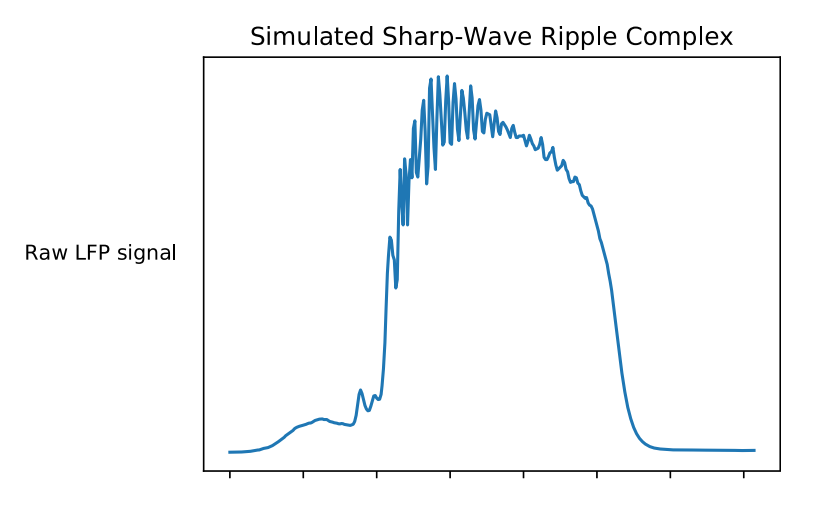
\includegraphics[width=0.75\linewidth]{images/Sharp Wave Ripple Complex.png}
        \caption{Plot of a raw LFP trace \cite{Aussel.2018}}
        \label{fig:sharp-Wave-Ripple}
    \end{figure}


    \subsection{Automated Sharp Wave Ripple Detection}
    
    The occurrence and properties of sharp wave ripples are the most important aspects of the output for this thesis. Their automatic identification and analysis are therefore essential, to allow for an efficient evaluation of different brain states. Unfortunately, a common standard for this procedure, which comes with several methodological challenges, is nonexistent \cite{Liu.2022}. As a consequence, the analysis of this work is in large parts based on the approach presented by \textcite{AmelieAussel.2020}, that already was used with the model. However, a few thresholds and procedures had to be adjusted to accommodate the employed model configuration and use case.\\
    The resulting detection algorithm can be divided into two stages. The \textit{detection of the sharp wave}, followed by the \textit{frequency analysis}, which analyzes candidate waves (also called events) for a superimposed ripple.
    
    % Detecting sharp wave
        % with help of rms standard deviation
            % unusual strong signal
            % exeeding a threshold that can be defined
                % is parameter that needs to be configured
                % mention specific values used
    To detect the large amplitude deflection of a \textbf{sharp wave}, the signal's root mean square (RMS) is calculated, based on non-overlapping time windows of 10ms. These RMS values are a reference for the signal power \cite{glaser.2012}. Then their standard deviation (SD) is extracted, which can be used to identify unusually strong signal portions. For a signal portion to be considered a sharp wave, its RMS values must be larger than 3 times the SD, reaching a peak of at least 4.5 times the SD.\\ 
    % checking if the strongest frequency in sharp wave is ripple
        % extracting spectral density
            % which frequency has how much power
        % range of qualifying peak frequncy is parameter
            % was chosen to be ...
    The sharp waves identified like this, then need to be \textbf{analyzed in} terms of their \textbf{power spectrum}. This is performed by first bandpass filtering the signal parts between 30 and 400Hz (employing a Butterworth filter of second order) and therefore discarding especially the lower frequencies of high power. Followed by the extraction of the frequency of the highest power in the remaining range. This \textit{peak frequency} is the most relevant oscillation pattern imposed on the sharp wave and defines, whether it qualifies as a ripple or not. For this work, the frequency range, supposed by \textcite{vanQuyen.2010} was used, defining every sharp wave with a superimposed peak frequency between 100-250Hz, as a sharp wave ripple (complex).
    

 
\section{Electromagnetic Attacks}
% general elaborations on attack design
% Because no specific proposal for the simulation of such an attack exists
    % Exploring different mechanisms that could lead to the observed symptoms
        % first evaluate the relevance of each aspect
        % propose and evaluate possible combinations that could represent a full attack
% (as foundations showed) different categories of mechanisms exist
    % specifically Neurotransmitter changes, Structural damage and alterations of input identified as promising and will be explored
    As discussed in the previous chapter, the topic of Neurostrikes is very novel, and their inner mechanisms are not fully understood. As a consequence, also no specific proposals on the integration of such an attack in a brain simulation exist. Therefore, this work explores potential underlying mechanisms that could be responsible for the symptoms associated with Neurostrikes. Focusing primarily on the reported memory and learning impairments, to establish a basis for further research and the development of countermeasures.\\
    Different mechanism categories have been identified, that could be involved in such impairments. Specifically \textit{changes in neurotransmitters} and \textit{structural damage} to the hippocampus showed promising connections to both electromagnetic radiation and memory performance. How each of these categories was designed, will be presented below. Followed by the discussion and proposal of combinations of them, resulting in full-scale attacks. 


    \subsection{Neurotransmitter Changes}
    % As hu showed, influence of rf emr on neurotransmitters well documented
        % has to be stated that the results are not uniform
        % might be caused by large radiation parameter variability between experiments
    % Changes in acetylcholine seem to have an impact on memory consolidation Hu.2021, Aussel.2018
    % papers like Fujiwara.1978, Hu.2021  idnetified an increase of it
        % specifically 1.2x - 2.5x (Fujiwara.1978)
    % since Aussel also investigated ACh levels in model, integration easy
        % adjustment of parameter values (gCAN and G_ACh)
            % mention their impact
        % realistic value range based on observed level change
            % top level metioning of literature and resulting range
    
    As \textcite{Hu.2021} showed, RF EMR can have an impact on many neurotransmitter levels in the brain. However, the specific results of different studies are not uniform, which the authors attribute to the large variance in parameters and conditions of the experiments.\\
    Especially the neurotransmitter acetylcholine is of interest for this work, as it is affected by RF EMR \cite{Hu.2021} \cite{Fujiwara.1978}, and is associated with memory processes \cite{Aussel.2018}. Specifically, an increase in this neurotransmitter has been reported \cite{Hu.2021}, which as \textcite{Fujiwara.1978} found can manifest in up to 2.5 times the concentration, compared to the standard values of the waking state.\\
    The integration of such changes into the simulation is already supported by the model, as the acetylcholine levels were already a parameter of interest for the model creators \cite{Aussel.2018}. They investigated the varying concentrations across the sleep-wake cycle and realized their effect with the help of the parameters \textit{gCAN} and \textit{gACh} \cite{HippSimModel.2}. Whilst \textit{gCAN} represents the conductance of a "Calcium-Activated-Nonspecific" (CAN) ion channel \cite{Aussel.2018}, \textit{gACh} defines a factor that influences a series of synaptic conductances inside sub-regions of the hippocampus. More specifically, it increases both the excitatory synaptic conductances inside the DG, as well as the inhibitory synaptic conductances in the DG and CA1 region. Conclusively, \textit{gACh} also decreases the excitatory synaptic conductances inside the EC and CA3 region \cite{AmelieAussel.2020}.\\
    In the context of their work, \textcite{Aussel.2018} defined two values for each of the parameters, representing the sleep or waking state respectively (\(gCAN : [0.5\mu S/cm^2, 25\mu S/cm^2]\), \(gACh : [1, 3]\)). These values need to be associated with a concentration of acetylcholine, to be able to define realistic values for the simulation of an attack. Due to a lack of comparable absolute values, this was done with relative observations. \textcite{Hasselmo.1999} states that the neurotransmitter level during sleep is about a third of the one during the waking state. Combined with the findings of \textcite{Fujiwara.1978} (documenting an increase due to radiation of up to 2.5 times relative to waking concentrations), this work concluded that an attack during the sleeping state, could result in similar levels as the ones during waking state (\(gCAN = 25\mu S/cm^2\), \(gACh = 3\)). However, since these estimations are based on observations, of which the comparability, robustness, and precision are very limited, a range of values was explored nonetheless to allow for more meaningful evaluations. The waking values constituted thereby the strongest deviation of the sleeping values and upper bound of the explored range.
    

    \subsection{Structural Damage}
    % result from rf emr
    % influence learning and memory
    % specific magnitude of changes
    % how integrated
    Different forms of structural damage have been observed as a consequence of electromagnetic radiation \cite{Shahin.2015} \cite{Tan.2017}. Due to the employed model, those affecting the hippocampus are of particular interest for this work. Also because damages affecting this brain area, are considered as a potential cause of memory and learning impairments \cite{Narayanan.2019}. Specific observations reported \textit{damage to neurons} \cite{Shahin.2015} \cite{Altun.2017}, but also \textit{damage to synapses} \cite{Tan.2017} \cite{Xu.2006}.
    
    Concerning affected \textbf{neurons}, \textcite{Shahin.2015} reported an increase in both neuronal but also non-neuronal cell deaths, following the exposure to 2.45GHz (RF \cite{BORTKIEWICZ.2019}) radiation. These findings were supported by the observations of \textcite{Altun.2017}, who further quantified the observed neuron reduction in the whole hippocampus to be 40\%. Although, it has to be stated that this reduction was measured after long-term exposure (1 hour every day for 15 days).\\
    Integrating such a reduction of neurons into the simulation is also already facilitated by a parameter of the model (\textit{N}). It defines the maximum amount of the largest excitatory neuron groups and scales the others proportional to this value \cite{HippSimModel.2}. Its standard value is 10'000, resulting in the amounts displayed in table \ref{tab:population_sizes}. For example, a 10\% reduction to 9'000 would also result in a 10\% reduction of all the other values. To also asses less severe states like the one documented by \textcite{Altun.2017}, the whole range from 6'000-10'000 neurons will be explored. 

    \begin{table}[h]
        \centering
            \begin{tabular}{@{}lcc@{}}
                \toprule
                Region & $N_E$ & $N_I$ \\ 
                \midrule
                Entorhinal cortex & 10'000 & 1'000 \\
                Dentate Gyrus & 10'000 & 100 \\
                CA3 & 1'000 & 100 \\
                CA1 & 10'000 & 1'000 \\ 
                \bottomrule
            \end{tabular}
        \caption{Number of excitatory neurons (\(N_E\)) and interneurons (\(N_I\)) in each region \cite{Aussel.2018}}
        \label{tab:population_sizes}
    \end{table}
    

    Damage to \textbf{synapses} in the hippocampus was characterized by \textcite{Xu.2006}, stating that 1.8GHz radiation, might lead to reduced synaptic activity and synapses in general. However, more specific findings were the amplitude reductions of excitatory postsynaptic currents. This finding was also quantified and amounted to a reduction of 20\%.\\
    To integrate this effect into the simulation, the model parameter \(g\_max\_e\) is perfectly suited, as it defines the maximum conductance of all excitatory synapses. Since its standard value is defined as \(60pS\), a 20\% reduction would amount to \(48pS\) which represents the lower bound of the explored value range for this parameter. 


    %\subsection{Input Alterations}
    %Since the impact of radiofrequency electromagnetic radiation is not restricted to the hippocampus \cite{Lai.1994}, the stimuli reaching the structure most likely are altered as well. These alterations, would for example reflect a decrease of spontaneous activity as documented by \textcite{seaman1978slow} and \textcite{wachtel1975effects}.\\
    %To integrate such a reduced activity, different parameters of the input can be adjusted. For example, the measurement amplitude or frequency to which the measurements are scaled could be reduced. Exact values are in this context difficult to specify theoretically, which is why also for this type of mechanism, a range of values in these parameters will be explored.

    \subsection{Full Attack}
    To represent a full-scale attack, these mechanisms and adjusted parameters can simply be combined to different extents. This enables a type of worst-case scenario, where all parameters are applied at their extreme values, but especially the exploration of a more realistic brain state under attack, as these mechanisms will most likely not be triggered selectively.\\
    Guided by the relation between radiation intensity and its effect on the brain, the \textit{Full Attack} will be explored with parameter combinations, that could arise from the same level of radiation exposure. This was achieved by defining 4 different intensity steps across the value range of every parameter, where the highest value represents the strongest deviation from the healthy sleep values in the range. Values of the same intensity level were then combined, to simulate different levels of overall radiation intensity. 


%\section{Countermeasure}

\chapter{Implementation} % ~ 10 pages
\label{chap:implementation}
% Documentation of my code implementations
This chapter presents and explains the most important implementations of this work, including only what is relevant to the contribution of this work. Thereby, a connection between the theory of the previous chapter and its technological realization shall be made, while focusing mostly on the high-level functionality of the code.\\
According to the simulation model, all the developed functionalities were written in Python \cite{van1995python}. This includes the synthetic input generation, the output analysis, as well as some code related to the attack integration, which is presented in this order. 


\section{Synthetic Input}
% Mention goal and approach to this section
    % developed in 1. model version
The necessity of a synthetic input generation function arose in the context of the first model version \cite{HippSimModel.1}. It was therefore implemented and later integrated into the corresponding model code.

    %\subsection{Generation Function}
    % General approach
        % recreated input equation from design
        % but tried to replace realistic approach and code seamlessly
            % translated into frequency
        % evaluation of results lead to addition of
            % wave_realization_interval and according function
            % integration of variable noise scaling
        % fixed values for parameters that are fixed in model
            % sampling frequency
        % made rest a parameter
    As discussed in the design chapter, this implementation is based on the works of \textcite{Aussel.2021}, who proposed an equation for synthetic input. However, the implementation was adjusted to fit seamlessly into the existing code. Primarily resulting in the decision to not integrate the input by injecting a current into the stimulated neurons, but rather translate the input equation into frequencies that define the firing rate of those neurons. Since such a translation of a stimulus pattern into firing frequencies of neurons is also performed with the realistic input files, it was possible to adapt some aspects of the approach there and then supply the model with the same type of input parameter. This further avoided the necessity of more fundamental changes to the model, which would have been hard to validate.\\
    The developed function includes the "is\_in\_correct\_cycle" parameter and therefore is an algorithmic representation of the second equation presented in the design. Values like the sampling frequency that are tuned to the model configuration were defined inside the function whilst everything else remained a variable parameter.\\

    \begin{lstlisting}[caption={Generate Input Function}]
    def generate_input(A1, f1, wave_realization_interval, sim_time):
        
        record_dt = 1. / 1024 * second  # Sampling interval
        t0 = 0.250  # Start time of input
    
        # Array of sample times
        times = np.arange(0 * second, sim_time, record_dt)
    
        # Generate square wave
        input_values = np.zeros_like(times)
    
        def is_in_correct_cycle(input_frequency, current_time, wave_realization_int):
            ms_per_cycle = 1 / input_frequency
            wave_number = int((current_time - t0) / ms_per_cycle)
            return wave_number % wave_realization_int == 0
    
        for i, t in enumerate(times):
            if t >= t0 and np.sin(2 * np.pi * f1 * (t - t0)) >= 0 and is_in_correct_cycle(f1, t, wave_realization_interval):
                input_values[i] = A1
    
    
        # Normalize values to range [0, 1]
        input_normalized = (input_values - min(input_values)) / (max(input_values) - min(input_values))
    
        # Add noise
        input_noisy = (5 / 6) * input_normalized + (1 / 6) * np.random.rand(len(input_normalized))
    
        # Scale to a maximum frequency of 200 Hz
        max_rate = 200 * Hz
        input_scaled = input_noisy * max_rate
    
        input_timed = TimedArray(input_scaled, dt=record_dt)
    
        return input_timed
    \end{lstlisting}
    The parameters of the function allowed for the adjustment and exploration of all important aspects of the input. Whilst \textit{A1} and \textit{f1} represent the same values that can be found in the input equation, the \textit{wave\_realization\_interval} stands for \(w\). Further, the \textit{sim\_time} parameter was necessary to represent the configured simulation runtime in seconds and ensures that the input is generated in the required length. The function returns a brian2 "TimedArray", containing an input frequency at every sample time step. This array could then be used to replace the ones that would otherwise be created from realistic input files. 

    %\subsection{Realistic Input Integration}?


\section{Output Analysis}
% Connect to Design section
% mention i based it on Event_detection_Aussel.py
    % changes i made
% explain structure of section
    % sharp wave detection function
    % event detection function employing it
From a technical standpoint, the output analysis incorporates two different procedures. First, the LFP data has to be processed, such that relevant aspects are revealed. Only then can the data be structured and displayed in a way that facilitates the extraction of relevant information.\\
The approach to the data processing was based on the works \textcite{Aussel.2018}, who supplied a basic event detection function in their first model code \cite{HippSimModel.1}. However, this code was altered significantly, to facilitate the data analysis of this work. For reasons of modularity and encapsulation, the procedure was split into two functions, that relate to the two SWR detection stages, mentioned in the design. The first one identifies sharp waves, whilst the second one analyses their superimposed oscillation frequencies. In the following, their specific implementations are presented.

    \subsection{Sharp Wave Detection}
    % general procedure
    % tell what subfunctions do
    Since the sharp waves are identified with the help of root mean square values of non-overlapping signal windows, these RMS values are calculated first. This was done with a helper function, to enhance readability of the code. Its standard deviation is then derived to specify the threshold condition values. Parts of the signal with RMS values higher than the boundary condition, exceeding the peak threshold at some point, qualify as sharp waves.\\
    
    \begin{lstlisting}[caption={Sharp Wave Detection Function}]
    def sharp_wave_detection(sig, boundary_condition, peak_condition, record_dt):
        # calculation of root-mean-square
        start_plot_time = 50 * msecond
        start_ind = int(start_plot_time / record_dt)
        sig_rms = window_rms(sig[start_ind:] - mean(sig[start_ind:]), int(10 * ms / record_dt))
        sig_std = std(sig_rms)
    
        boundary_value = boundary_condition * sig_std
        peak_value = peak_condition * sig_std
    
        # detection of sharp waves
        begin = 0
        peak = False
        all_sharp_waves = []
    
        for ind in range(len(sig_rms)):
            rms = sig_rms[ind]
            if rms > boundary_value and begin == 0:
                # event start
                begin = ind
            if rms > peak_value and not peak:
                # event fulfills peak condition
                peak = True
            elif rms < boundary_value and peak:
                # sharp wave detected
                sharp_wave_signal = sig[begin + start_ind:ind + start_ind]
                all_sharp_waves.append(sharp_wave_signal)
                begin = 0
                peak = False
            elif rms < boundary_value and not peak:
                # event without sufficient peak
                begin = 0
                peak = False
    
        return all_sharp_waves
    \end{lstlisting}
     % explanation of derived values/function output
     Next to the signal that is analyzed for sharp waves, this function accepts the boundary and peak condition values, defining them. This allows for the convenient evaluation of different values. Since the sampling interval \textit{record\_dt}, needs to align with external values, it was chosen to be a necessary parameter as well.\\
     The return value of the function, labeled \textit{all\_sharp\_waves}, contains lists of the identified sharp wave signals. Their further analysis and categorization is then performed by the following function. 

    \subsection{Event Detection}
    % general procedure, interesting aspects
    Whilst the main contribution of this function is the analysis of event frequencies and their power spectrum, it also serves as the main output processing function. It collects all the relevant data and structures it to facilitate its use by higher-level analysis and representation functions.\\
    In a first step, it retrieves the sharp wave event signals, with the help of the above-explained function \textit{sharp\_wave\_detection} (setting the boundary and peak condition values to \textit{3} respectively \textit{4.5}). Then it performs the frequency analysis of every event, just as specified in the design section. Employing the helper function \textit{frequency\_band\_analysis} in multiple instances.\\
    Given the \textit{low} and \textit{high}-frequency bound parameters, this function applies a band-pass filter to the \textit{event} and derives the power spectrum of the resulting signal. Leading to the output of a \textit{frequencies} and according \textit{power\_spectrum} list, as well as the \textit{filtered\_event} signal.\\
    This function is used at the beginning of the frequency analysis to restrict it to the relevant oscillation range. Then, general data regarding all events is collected, before sharp wave ripples are detected based on the \textit{peak\_frequency} (the frequency that contains the most power). In the end, the power spectrum of every event is derived in the theta, gamma, and ripple bands.\\
    % CODE
    \begin{lstlisting}[caption={Event Detection Function}]
    def event_detection(sig):
        # model specific signal properties
        sample_frequency = 1024 * Hz
        record_dt = 1 / sample_frequency
    
        event_signals = sharp_wave_detection(sig, 3, 4.5, record_dt)
    
        # frequency analysis
        filtered_events = []
        all_spectrum_peaks = []
        all_durations = []
    
        sharp_wave_ripples = []
        sharp_wave_ripple_peaks = []
        sharp_wave_ripple_durations = []
    
        theta_spectrum = []
        gamma_spectrum = []
        ripple_spectrum = []
    
        for event in event_signals:
            # filter in broad frequency range
            frequencies, power_spectrum, filtered_event = frequency_band_analysis(event, 30, 400, sample_frequency)
            if len(frequencies) != 0 and len(power_spectrum) != 0:
                # collect general event data
                filtered_events.append(filtered_event)
                duration = len(event) * record_dt * 1000
                all_durations.append(duration)
                peak_frequency = frequencies[argmax(power_spectrum)]
                all_spectrum_peaks.append(peak_frequency)
    
                # identify sharp wave ripples
                if 100 <= peak_frequency <= 250:
                    sharp_wave_ripples.append(event)
                    sharp_wave_ripple_peaks.append(peak_frequency)
                    sharp_wave_ripple_durations.append(duration)
    
            # collect power of frequency bands
            theta_spectrum.extend(frequency_band_analysis(event, 5, 10, sample_frequency)[1])
            gamma_spectrum.extend(frequency_band_analysis(event, 30, 100, sample_frequency)[1])
            ripple_spectrum.extend(frequency_band_analysis(event, 100, 250, sample_frequency)[1])
    
        # structure result data
        all_event_data = [event_signals, filtered_events, all_spectrum_peaks, all_durations]
        swr_data = [sharp_wave_ripples, sharp_wave_ripple_peaks, sharp_wave_ripple_durations]
        band_spectra = [theta_spectrum, gamma_spectrum, ripple_spectrum]
    
        return all_event_data, swr_data, band_spectra
    \end{lstlisting}
    The sampling frequency was chosen to be statically defined at the top of the function, as it remained the same overall performed simulations. Therefore only the LFP output signal, in the form of a list is required as parameter.\\
    The function output contains all the collected data, sorted and structured as shown in the last code section. Enabling a convenient extraction of relevant aspects for all further analysis and interpretation procedures. 
    
    On the data that is collected with these functions, a proper analysis still needs to be performed, to extract the information of interest. This includes, for the most part, the aggregation and comparison of multiple simulation outputs. But also the representation of important values in a way that facilitates their interpretation. For example with the help of graphs or well-organized text output. Implementations of this are however not directly related to the contribution of this work and are therefore omitted.


% \subsection{Analysis Functions}?
%     \subsubsection{Single Process Analysis}
 %     \subsubsection{Collection Process Analysis}


\section{Electromagnetic Attacks}
% As specified in Desing Chapter
    % Different types of attack implementations
        % most parameter based
        % some (input alterations) Algorithm based
    % Code wise not much to show for parameter based attacks
        % but general parameterization procedure shall be explained
    % Algorithms presented and discussed
As specified in the design chapter, electromagnetic attacks can be realized by adjusting many different simulation aspects. Their technical integration was however facilitated by the newer model version \cite{HippSimModel.2}, as it provides a large parameter space. This allowed all of the attacks to be realized with their help. Leading to very similar and simple implementations, of which only the general procedure and main aspects will be presented.

    %\subsection{Parameter-based Attacks}
    % Explanation of parallel Processing
    % Limited Code presentation
    % Mostly specification of parameter adjustment process and how programmatically realized
    The newer model version can be configured and executed with the help of 3 different files and related approaches. Two of them supply a graphical user interface with different levels of details that may be adjusted. However, they can only be used to initiate a single simulation configuration at a time. Therefore, exclusively the third option, utilizing the \textit{parallel\_processing.py} file, was used for this work.\\
    This approach enabled the scheduling of multiple simulation configurations, which depending on the available processor cores, were also executed in parallel. Thereby significantly increasing the simulation efficiency and amount of data collected. Ultimately allowing for a more robust and reliable evaluation of results. 

    The \textit{parallel\_processing.py} file mainly consists of parameter definitions, incorporating in total 25 different ones. Whilst some are used to define for example the input file location or simulation duration, others are related to neuron or network model aspects. In the following code snipped, all attack-related parameters are shown with their standard, respectively healthy value configuration.\\
    
    \begin{lstlisting}[caption={Example Parameter definition}]
    # Structural parameters
    liste_maxN = [10000] # number of excitatory neurons in the CA1 region (scaling the rest accordingly)
    liste_g_max_e = [60*psiemens] # maximum synaptic conductances of excitatory synapses
    
    # Acetylcholine (sleep/wake) parameters
    liste_gCAN = [(0.5*usiemens*cmeter**-2, 25*usiemens*cmeter**-2)] # (sleep CAN channel conductance, wakefulness CAN channel conductance)
    liste_CAN = ['sleep'] # choose between sleep and wakefulness CAN channel conductances
    liste_G_ACh = [3] # gain applied on some synaptic conductances under cholinergic modulation ('wake' functional connectivity)
    liste_functional_co = ['sleep']  # choose between sleep and wakefulness functional connectivity
    \end{lstlisting}

    As one can observe, every parameter is defined by a list, which allows the assignment of multiple values for it. When the simulation then is executed, the file will create a cross-product of all available parameter values, and schedule a simulation for it. This means every possible combination of list entries, across all the parameters, will be simulated. Also allowing for the definition of the same value multiple times, to collect more data on the same simulation parameters, with a single file configuration.

    
    %\subsection{Algorithm-based Attacks}
    
\chapter{Evaluation} % ~ 10 pages
\label{chap:evaluation}
This chapter presents and evaluates the simulation output of all the investigations that were performed with the model of the hippocampus \cite{HippSimModel.1} \cite{HippSimModel.2}. First elaborating on the initial work, with the synthetic input, before a short overview of the output analysis and its relevance is supplied. After that, the most extensive analysis is performed on the attack-related simulations. 


\section{Simulation Input}
    This section is concerned with the different versions of model input, that were used throughout this work. That includes the synthetic input, that was created and used in the beginning, as well as EEG files that later were used as its alternative.\\
    The synthetic input was developed and evaluated with the first version of the model code \cite{HippSimModel.1}. Therefore, the output analysis and reference results were derived from the paper associated with the same model version \cite{Aussel.2018}, ensuring the best possible comparability.\\
    These reference values will be presented before more details about the synthetic input and its alternative are discussed. 


    \subsection{Reference Output Values}
    % Estabilish baseline (sollparameter)
        % values of paper
            % LFP Plots during sleep
            % Event parameters (Sharp wave ripples)
                % values they derived with realistic 
    Before the simulation output can be interpreted and properly evaluated, it is necessary to elaborate on the analyzed aspects and present the reference values that were considered to be realistic. Generally, the input was assumed to be better, the more similar its output was to the values, that were derived from the original works of \textcite{Aussel.2018} (see Figure \ref{fig:input_reference}).
    
    \begin{figure}
        \centering
        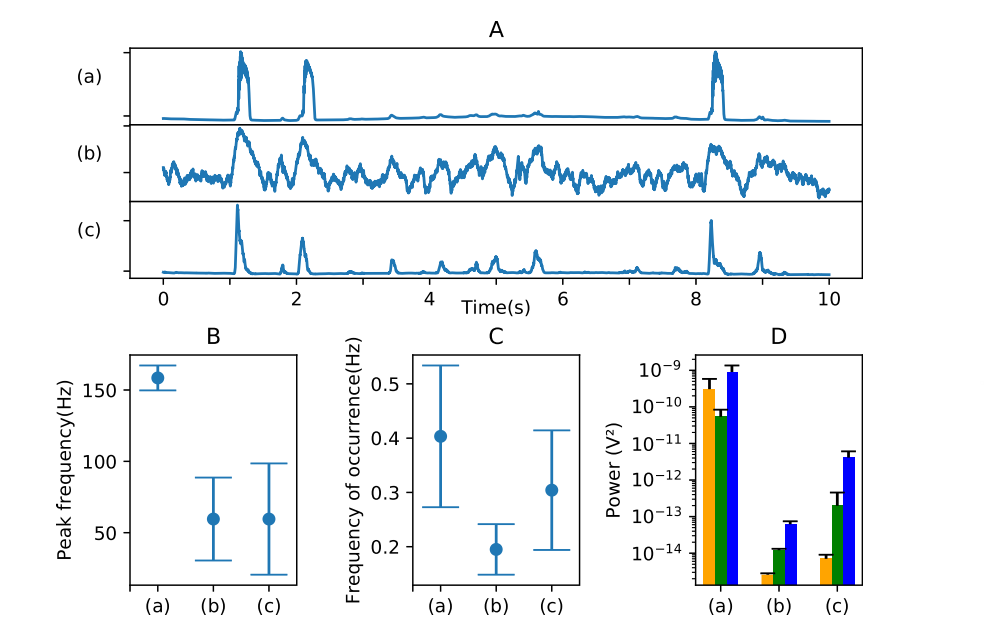
\includegraphics[width=1\linewidth]{images/Sleep Input reference Figure Aussel.2018.png}
        \caption{Main reference graphs derived from \textcite{Aussel.2018}, showing the model behavior during sleep in different network settings. Values of \textbf{(a)} were considered for the evaluation of the input, as they were produced in the realistic network configuration, employed by this work. The other values represent the model behavior in a less realistic connectivity \textbf{(b)} or topology \textbf{(c)} setting. \textbf{A:} LFP signal, plotted over time. \textbf{B:} Peak frequency of detected events. \textbf{C:} Event occurrence frequency. \textbf{D:} Power in the ripple (120-200Hz, yellow), gamma (30-100Hz, green), and theta (5-10Hz, blue) oscillation frequency bands.}
        \label{fig:input_reference}
    \end{figure}
    
    The most fundamental output analysis was performed on the raw \textbf{LFP} time series, constituting the unprocessed simulation output. The values of these files represent voltages recorded with a sampling frequency of 1024Hz \cite{HippSimModel.1}. When plotted over time, it is possible to observe the general activity of the model. Graph \textbf{A} in figure \ref{fig:input_reference}, shows such a plot and represents the reference activity during sleep.\\
    However, more specific aspects of the model output need to be observed, to evaluate cognitive processes like memory formation. In this context, the investigation of certain activity patterns was performed, as presented in more detail in the design section. Specifically sharp wave ripples, consisting of a sharp wave (also labeled as events) with superimposed ripple oscillations (100-250Hz), could be related to the cognitive process.\\
    The strongest oscillation frequencies during a detected event (also labeled as "\textbf{peak frequency}"), therefore represent an important aspect of the simulation output. The reference values for this parameter, lie approximately between 150 and 165 Hz, as graph \textbf{B} of figure \ref{fig:input_reference} indicates.\\
    Since SWRs, fundamentally rely on the occurrence of \textbf{events}, their general occurrence frequency is of central importance as well. Based on graph \textbf{C}, this work considered values between 0.3 and 0.5Hz as realistic, translating into 18-30 events per minute.\\
    Lastly, the power spectrum of detected events was also analyzed in a more general way. By deriving the mean power of the ripple, gamma, and theta frequency bands, the overall power distribution can be observed. A realistic distribution is shown in graph \textbf{D} of figure \ref{fig:input_reference}, where the ripple and theta bands, carry more power than the gamma band.

        

    \subsection{Synthetically Produced Output}
    With the input generation function, presented in the implementation chapter, a series of parameter values were explored. Specifically, the influence of frequency, amplitude, and wave realization interval on the model behavior was investigated. First, the most relevant observations concerning every parameter will be shown and discussed, before the most realistic parameter value combination is identified and evaluated. After that, some important implications of these findings on SWRs and their properties will be summarized. 
    

        \subsubsection{Parameter Analysis}
        % Amplitude 
            % no significant influence due to normalization
        Evaluating the importance of every parameter, it quickly became apparent, that the \textbf{amplitude} parameter \(A_1\), did not have any significant impact on the simulation results. This could be attributed to the way that the input equation was implemented. Specifically, in the process of translating the amplitude values into Frequencies, their magnitude is lost through normalization. Whilst this was done to ensure a maximum value for the stimulation frequency of 200Hz, it rendered the parameter useless. Nonetheless, all further investigations were performed with a uniform amplitude value of 1.
        
        % frequency influence
            % two extreme examples (F5, F1, F0.1) -> LFP graphs
                % scales event occurence
                % no more power and events at to high value
        Running the simulation with a series of \textbf{frequency} values, revealed a strong relationship between the generated input and resulting LFP values. This can be well observed in figure \ref{fig:input-LFP-comp-0.1_5}, comparing the LFP plots of two simulations with different frequency values. Whilst some activity deviates from the square wave pattern, the general shape can still be recognized. The activation phases further seem to be occurring at the same (or very similar) frequency as specified by \(f_1\).\\
        \begin{figure}[htbp]
            \centering
            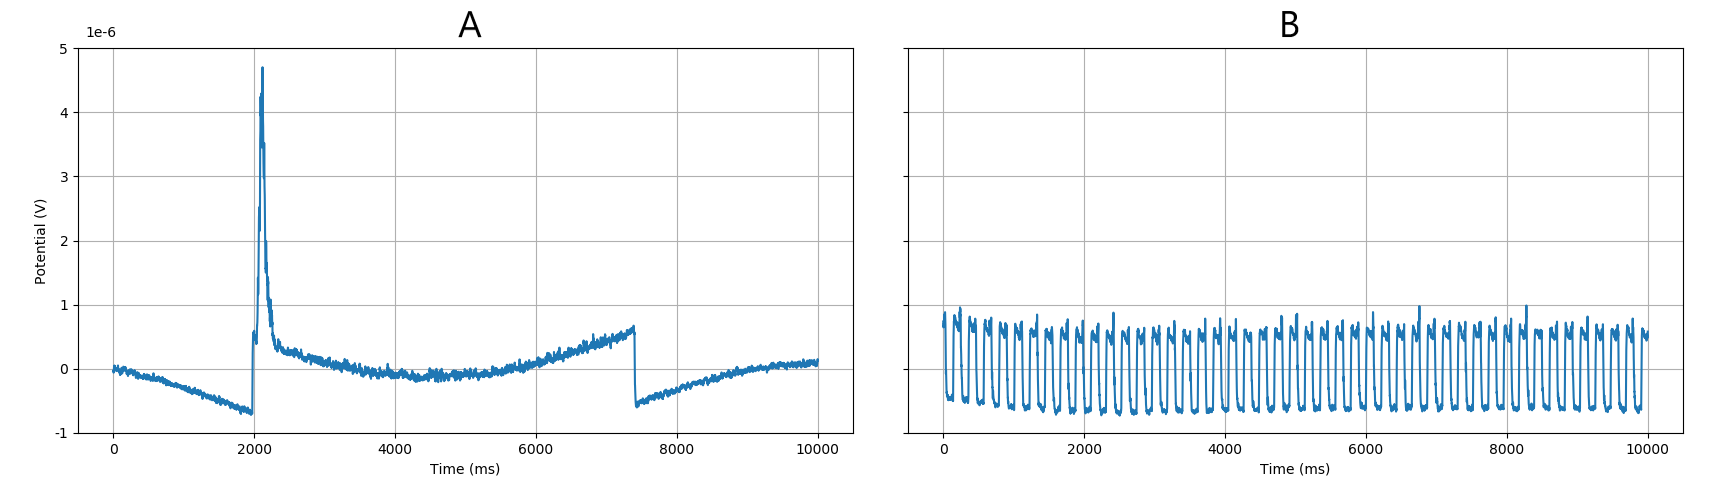
\includegraphics[width=1\linewidth]{images/Input_LFP_f01-5_labeled_only.png}
            \caption{Comparison of two 10-second LFP traces, with different input frequencies. Illustrating the impact and relevance of parameter \(f_1\), by employing fixed values for the remaining parameters (\(A_1 = 1, w = 1\)). \textbf{A:} \(f_1 = 0.1Hz\). \textbf{B:} \(f_1 = 5Hz\)}
            \label{fig:input-LFP-comp-0.1_5}
        \end{figure}
        A similar observation was made regarding the event occurrence, which correlates strongly with the number of activation phases and therefore also with the input frequency. However, it was found that if the frequency was too high, almost no more events were detected. For example during simulation \textbf{B}, figure \ref{fig:input-LFP-comp-0.1_5} (configured with an input frequency of 5Hz), events only occurred at the beginning and end of the simulation, but not during the high-frequency stimulation phase. The few events that occurred further showed poor peak frequency values (with a mean of 16Hz) and carried almost no power in all three, but especially the ripple frequency band.
        
        % wave realization interval
            % Example: F=1, A=1 with W=1,2,3,4
            % influence mostly on event occurence -> plot depending on W
                % also large jump in power and frequency from 1-2 later more stable
                % allows for higher power and peak frequency through pause
        Initial explorations of the \textbf{wave realization interval} (\(w\)) parameter, were performed with fixed values for the input frequency and amplitude (\(f_1 = 1, A_1 = 1\)). Like this, the effects of the parameter were isolated, revealing a large impact on all the aspects presented in the previous section.\\
        \begin{figure}[htbp]
            \centering
            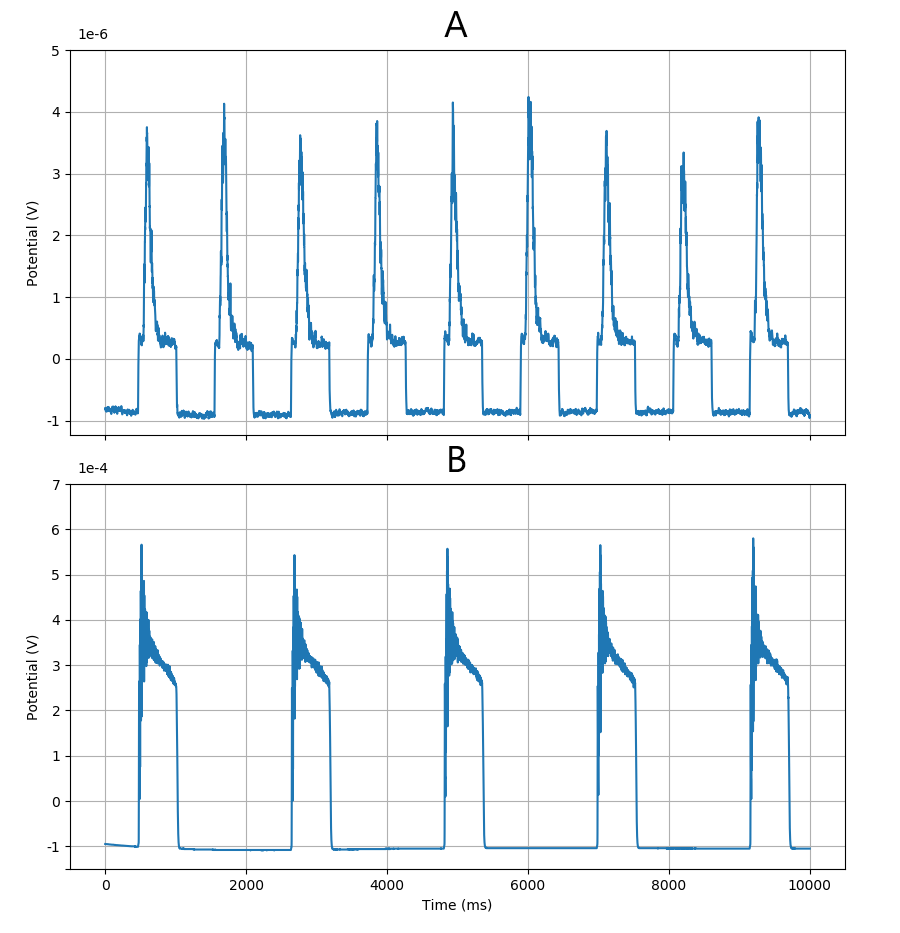
\includegraphics[width=0.5\linewidth]{images/lfpComp1-2.png}
            \caption{Two 10-second LFP traces, representing the isolated influence of the wave realization interval \(w\), with remaining parameter values of (\(A_1 = 1, f_1 = 1\)). \textbf{A:} \(w = 1\), not affecting the base input. \textbf{B:} \(w = 2\), realizing only every second input wave.}
            \label{fig:lfp_wave_int}
        \end{figure}
        
        Coinciding with the observations made in the context of the input frequency, the LFP traces reflect the input values very closely. As illustrated in figure \ref{fig:lfp_wave_int}, the reduction of input waves is directly translated into the same reduction of activity phases, measured in the LFP signal. However, the LFP plots already indicate a larger impact of the parameter. Increasing \textit{w} from 1 to 2 not only changed the shape of detected waves but also increased their amplitude.\\
        Further changes were observed in output aspects, related to SWRs. Figure \ref{fig:input_w_events} illustrates the development of event occurrences (\textbf{A}), their peak frequencies (\textbf{B}), and power bands (\textbf{C}) for \(w: [1, 4]\).
        
        \begin{figure}[htbp]
            \centering
            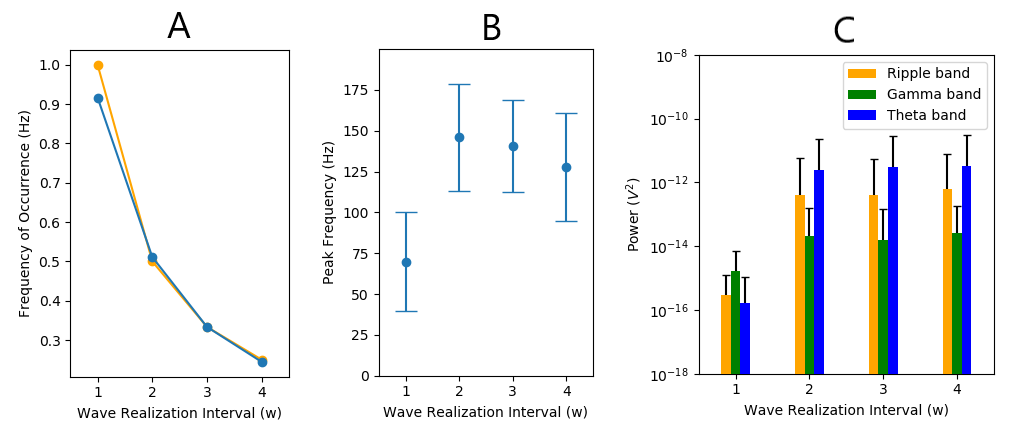
\includegraphics[width=1\linewidth]{images/input_w_labeled_event_plots.png}
            \caption{The impact of the wave realization parameter on the most important aspects of events. All data was collected from simulations with remaining input parameters: \{\(A_1 = 1, f_1 = 1\)\}. \textbf{A:} Shows the detected event occurrence frequency in \textit{blue}, compared to the frequency of realized input waves in \textit{orange}. \textbf{B:} Mean and standard deviation, of the highest power frequencies in detected events. \textbf{C:} The power of ripple (120-200Hz), gamma (30-100Hz), and theta (5-10Hz) frequency bands in detected events. Following the frequency ranges defined by the reference paper \cite{Aussel.2018}.}
            \label{fig:input_w_events}
        \end{figure}
        The event occurrence frequency is the parameter that changes most consistently with the value of \textit{w}. Plot \textbf{A} of figure \ref{fig:input_w_events} illustrates this continuous decrease, whilst also comparing it to the frequency of realized input waves. It can be observed that these two frequencies scale almost identically with the increasing values for \textit{w}. This aligns very well with the previous observations, indicating a strong coupling between the input waves, measured LFP activity phases, and the occurrence of detectable events.\\
        The other two graphs of figure \ref{fig:input_w_events} however, seem to show a different and less consistent effect of \textit{w} on events. One that is very similar to what was observed with the LFP amplitude, where the strongest changes happen between values 1 and 2. Whilst this step leads to the appearance of way more realistic values for both peak frequency and general power values, it does not scale with larger parameter values.\\
        These observations could for example be explained by a certain time threshold between these phases that must be reached before the network can produce a sufficiently strong activity event again. Such a necessity for refractory periods could further explain the observation,  that events cease to appear when the input frequency is too high.\\
        It was however not possible to explore more details regarding this effect, like specific threshold values, in the context and scale of this work.



        \subsubsection{Derived Input Parameter Combination}
        % Best result: F=1.5, A=1, wr=4
            % show stats
            % evaluate
        Throughout the exploration of the parameter space, it was possible to identify a combination of them, which yields \textbf{realistic values} for most aspects of the simulation output. Specifically by generating the sleep input with \textit{Amplitude} \(A_1 = 1\), \textit{input frequency} \(f_1 = 1.5\) and \textit{wave realization interval} \(w = 4\), the reference output values shown in figure \ref{fig:input_reference} could mostly be reproduced.
        \begin{figure}[htbp]
            \centering
            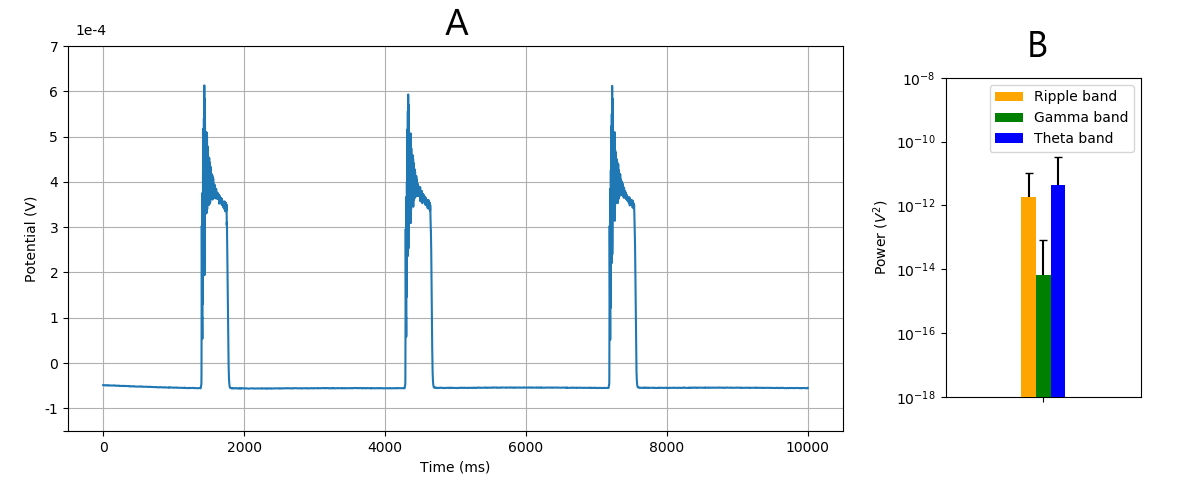
\includegraphics[width=1\linewidth]{images/BestLFPBands.png}
            \caption{Output generated with best parameter combination identified. \textbf{A:} 10-second LFP trace. \textbf{B:} Power in oscillation frequency bands (ripple (120-200Hz), gamma (30-100Hz), and theta (5-10Hz)).}
            \label{fig:best-input-plots}
        \end{figure}
        Resulting in the LFP plot and power bands of figure \ref{fig:best-input-plots}, which are quite similar to the reference regarding shape and power distribution. However, the power amplitude of all frequency bands is a bit lower than documented by \textcite{Aussel.2018}. The remaining event-related output aspects amounted to the following values:
        \begin{itemize}
            \item \textbf{Frequency of occurence}: 0.35Hz, or 21 events per minute, are very close to the mean value
            \item \textbf{Peak frequency}: 167Hz, which is just at the upper limit of the reference standard deviation, but within the bounds of all encountered ripple frequency band definitions.
        \end{itemize}
        Whilst all the reference values could be mostly reproduced with the above-presented input parameters, this synthetic input should not be considered a completely realistic alternative to EEG files. Especially since the presented reference values are only a collection of relevant, but not all output aspects. For example, the duration of detected events was not considered and unfortunately cannot be reproduced realistically with this input.
        
            
        \subsubsection{Implications on Sharp Wave Ripple Stimulation}
        % events occur with strong input injection
            % which by default and implementation details represents synchronus activation of many neurons
                % triggers 
        % high enough power and peak frequency only when
            % breaks long enough
            % than seem to scale with f
        The exploration of different input parameters showed some interesting correlations between input and SWRs. This section aims to summarize and evaluate these findings since they may guide the development of a countermeasure approach, based on brain-computer interfaces.
        
        In general, many findings showed a strong correlation between a large area stimulation of the entorhinal cortex by the input, the resulting LFP measurements, and the emergence of SWRs. This potential connection between brain stimulations and SWRs was however observed when the input was injected via the simulation of frequencies and not by currents. Implications on current injections that would be performed by BCIs are therefore limited.\\
        The second observation was that sufficiently strong events, with suitable oscillation frequencies, only occurred with long enough time intervals between them. This phenomenon might not only be restricted to frequency stimulation and should therefore also be considered in the context of brain-computer interfaces and current injections. 

            
        
    \subsection{Comparison to EEG Input}
    % own eeg file sim doesn't produce realistic ouput with their analysis function
        % may be different to the ones used in Aussel.2018
    % general differences and pros/cons observed
        % way more consistant and controllable "base case"
        % stereotypical behaviour of synthetic input
            % strong coupling to output
        % implications on real brain questionabel
            % due to big difference
    Exploring a synthetic input not only allowed for the exploration of its effects on SWRs but also enabled a comparison to EEG files. This shall provide an overview of both options and evaluate their suitability for different brain simulation contexts.\\
    Simulations that were performed with the later received EEG files, yielded LFP measurements that were completely unlike anything \textcite{Aussel.2018} presented as simulation output in this primary paper (see figure \ref{fig:EEG-LFP}). Even though they were performed using the same model code. Lacking any other indications, this is attributed to the fact that the received EEG files stem from later research and may differ from what was used in the reference paper.
    \begin{figure}[htbp]
        \centering
        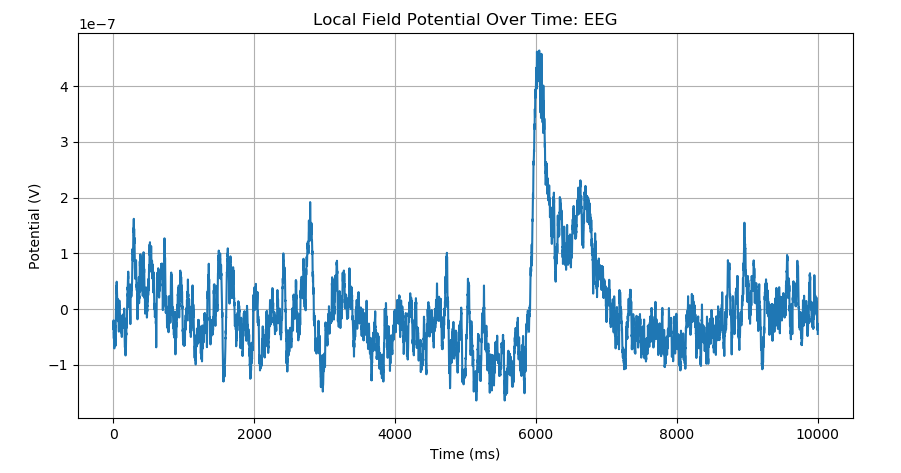
\includegraphics[width=0.75\linewidth]{images/EEG-LFP.png}
        \caption{10-second LFP trace, produced with EEG files as input.}
        \label{fig:EEG-LFP}
    \end{figure}
    Apart from the apparent differences in the LFP trace of the output, some more general observations were made in the process of working with both input types. The simulation behavior with synthetic input is for example more consistent. Resulting in smaller differences in the output values, across multiple simulations of the same configuration. This allows findings to be easier to reproduce and can reduce the amount of necessary simulations, to achieve robust mean values. This makes this option more viable if computational resources are sparse.\\
    However, the synthetic input produces rather stereotypical simulation behavior, which is strongly coupled to the specified input values. This does give a lot of control over a further parameter of the simulation but also makes related design choices extremely impactful. Consequently, a lot of research should be performed to ensure it produces realistic behavior across all relevant aspects of the simulation. Otherwise, it is questionable whether related findings have any implications on the real brain.\\ 
    By deriving the input from EEG files and therefore actual brain activity, this issue can be minimized. Making it the preferable option to perform realistic simulations and derive relevant findings. 
    


\section{Output Analysis}
% Necessary since 
% Massive impact on results
The output analysis is a core factor of the evaluations performed in this work. The values it extracts from the simulation output depend on a set of detection thresholds and frequency ranges. This section evaluates its influence on the simulation results and shows the impact of its main parameters.

% influence of peak/boundary condition
    % comparison graphic, peak distribution and duration
    % higher peak condition -> fewer false positives (shape-wise) but missing many
    % boundary condition -> strong influence on event length
    % frequency range - plot peak distribution
\begin{figure}[htbp]
    \centering
    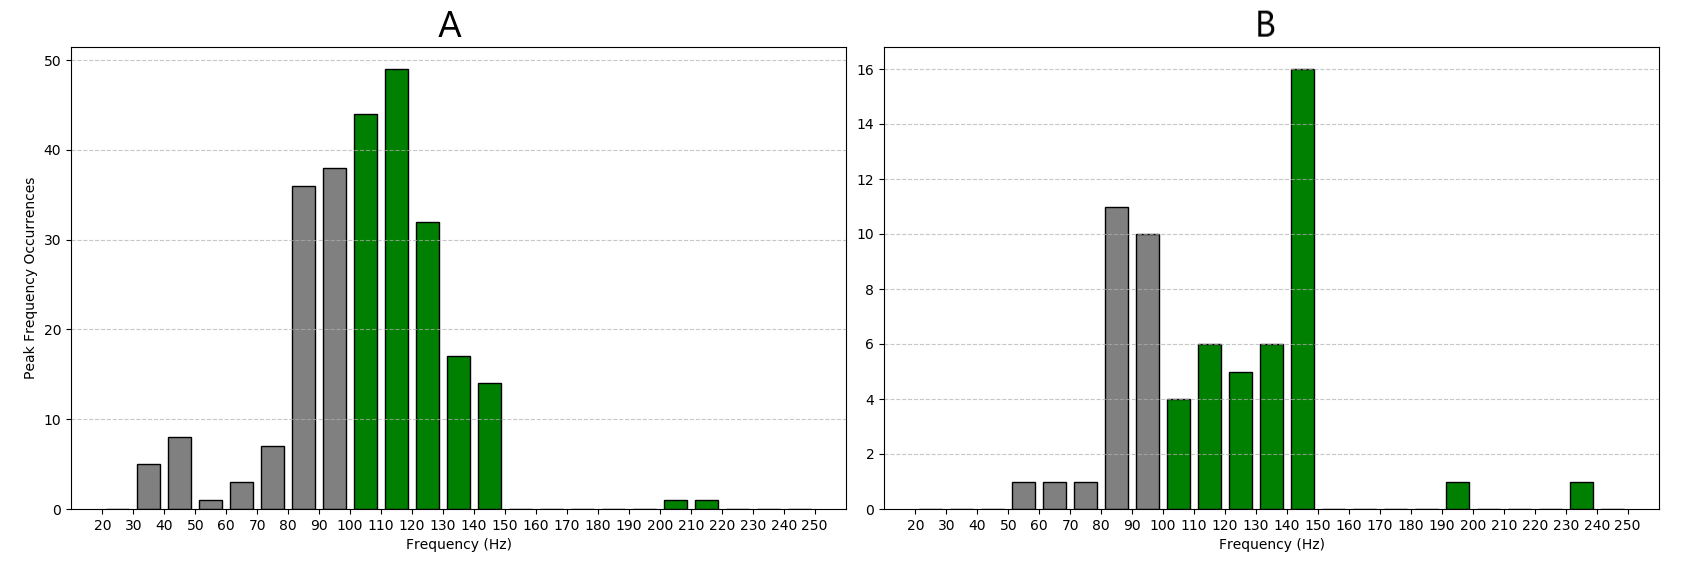
\includegraphics[width=1\linewidth]{images/Output Analysis Comparison.png}
    \caption{Event peak frequency distributions, derived from the same simulation data with different analysis parameters. Green bars represent occurrences in this work's ripple frequency range definition (100-250Hz). \textbf{A:} Derived with parameters used for remaining work (\(boundary\_condition\) = 3 x SD, \(peak\_condition\) = 4.5 x SD). \textbf{B:} Derived with boundary condition of 2 x SD and peak condition of 5.5 x SD}
    \label{fig:output_analysis_comp}
\end{figure}
A series of \textit{boundary conditions} (ranging from 2-4 x SD) and \textit{peak conditions} (ranging from 3-6 x SD) were explored in different combinations. This allowed the identification of their general influence on analysis results. This included the observation and comparison of event peak frequency distributions (like the ones depicted in figure \ref{fig:output_analysis_comp}), but also the inspection of LFP traces from detected events. The latter approach was mostly used to identify false positives (events that were detected but did not resemble a sharp wave ripple).\\
Concerning the \textbf{peak condition}, it was observed that with higher values, the ratio of false positives in detected events decreased. However, this trend was accompanied by a strong decrease in overall detected events (with almost none at a value of 6). This therefore also caused the analysis to miss many sharp wave ripples of smaller power.\\
The \textbf{boundary condition} had its strongest influence on the length of detected events. Increasing the duration of detected sharp waves, the lower its factor was chosen. Interestingly, the amount of detected events also correlated with the factor. Reaching its maximum around a factor of 3, before it decreased again with larger values.

% Why did i choose the ones I did
    % yielded realistic SWR stats in healthy condition
    % whilst not too many false positives
        % proper shape
Based on these observations, the best-suited parameters for the output analysis of this work were identified as: \(\{peak\_condition = 4.5, boundary\_condition = 3\}\). Even though these values are below the thresholds, stated to be used by \textcite{AmelieAussel.2020}, they produced the best analysis output. Yielding reasonable SWR values from healthy simulations, whilst avoiding too many false positives. Also, the results extracted with them are more robust to different definitions of the ripple frequency range, than others. This is a valuable property, considering the major differences between them.



\section{Electromagnetic Attacks}
% Effects of electromagnetic attacks on the hippocampus
    % simulating changes in the brain that are associated with rf emr
        % with a range of severities
        % comparing output to healthy baseline
    % What effects that might have on memory consolidation
% structure of section (and research approach)
    % Baseline of healthy sleep outputs
    % Mechanism-wise impact analysis (with same structure for all of them)
        % neurotransmitters, structural damage
        % The same output analysis and reference plots are provided for every scenario
            % allowing for a good comparison of parameter effects
    % Concluding with investigations of full attack (all mechanisms combined)
The core contribution of this work is to explore the underlying mechanisms of electromagnetic attacks, to establish a basis for countermeasures. Therefore, a series of brain alterations associated with RF EMR were identified and integrated into the simulation. Since the extent of alterations depends on the irradiation intensity and such values could not be identified for Neurostrikes, these alterations were explored in different severities. The resulting output was then compared to the healthy model behavior, focusing on network activities related to memory consolidation. Ultimately assessing the potential involvement of the explored mechanisms in Neurostrikes, by comparing their effects on cognition with the reported attack symptoms.\\
This section is therefore structured as follows. First, the healthy sleep activity of the model will be presented, to establish a baseline in the most important aspects. Then, two different mechanisms are investigated, based on two parameters each. Employing the same analysis structure and output representations for each simulation configuration, to facilitate their comparison. Lastly, the combination of all explored attack parameters will be evaluated in the context of a more realistic representation of Neurostrikes.

    
    \subsection{Healthy Sleep}
    % Establish a baseline of research parameters during healthy sleep
        % Necessary due to adjusted output analysis
        % Exclude any potential differences from paper reference, that could arise due to the simulation environment
    The output values presented in this section were produced with the second model version \cite{HippSimModel.2}. This model code was configured to represent a healthy sleeping configuration, and EEG files were used as input. To extract event-related data from the LFP output signal, the above-presented analysis function was employed. Doing so made it possible to establish a healthy reference value, with the exact same environment that later was used to simulate and analyze electromagnetic attacks. This ensures that potential alterations of behavior and output can solely be attributed to the attack-related parameter adjustments.\\
    In the following, the simulation results will be presented and discussed. Differentiating them also from findings made in the older model version and comparing them to relevant reference values of the model creator.

    % Plots:
        % LFP
        % Event peak frequency distribution
        % SWR Peak frequency
        % Power spectral band
    \begin{figure}[htbp]
        \centering
        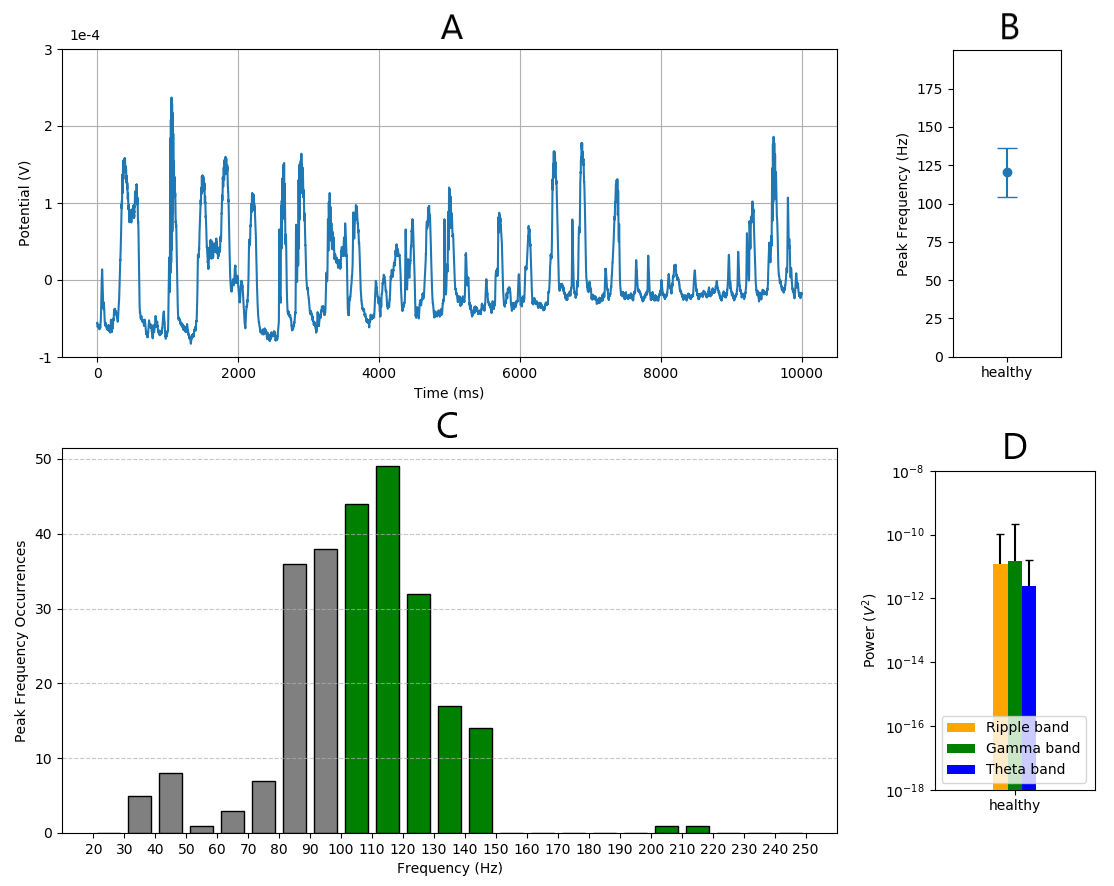
\includegraphics[width=1\linewidth]{images/attack_results/healthy_sleep_collection.png}
        \caption{Some graphical representations of the simulation output and its aspects, derived from 14 healthy sleep simulations of 60 seconds. \textbf{A:} Example of a 10-second LFP trace. \textbf{B:} Mean and standard deviation of the peak frequencies during sharp wave ripples. \textbf{C:} The distribution of peak frequencies across all detected events. Those falling in the ripple band (100-250Hz) are depicted in green and were considered sharp wave ripples. \textbf{D:} The power of detected events, analyzed in three separate frequency bands (theta: 5-10Hz, gamma: 30-100Hz, ripple: 100-250Hz).}
        \label{fig:healthy_collection}
    \end{figure}
        
    % Outputs generated on own machine
        % Short discussion of values
            % LFP different form reference for input, but way less stereotypic
            % distribution shows detected vs. selected events = swrs
        % very similar event outputs as aussel.2020
            % SWR peak freq 124 Hz vs. 125 Hz
            % SWR Occurrence 11.2 -> 0.18Hz vs. 11
        % except my events are shorter
            % SWR Duration 94 ms
            % but is consistent with swrs presented by Buszaki.2015
    The values depicted in figure \ref{fig:healthy_collection} give an overview of the general model behavior and describe the same or similar aspects, as the input reference (figure \ref{fig:input_reference}). However, the values are quite different from what the first model produced. The LFP measurements show less stereotypical behavior, and the event-related aspects differ a lot as well. Since \textcite{AmelieAussel.2020} reports very similar values with the new model version, these differences seem to be code-related.\\
    More specifically they reported a mean peak frequency of 125Hz, with a standard deviation of 20Hz, which is almost identical to the produced values shown in \textit{B}. Also, the \textbf{occurrence frequency} of 11 events per minute (~0.18Hz) aligns perfectly with the analysis results of \textbf{11.2 events per minute}. Only the sharp wave ripple \textbf{event duration}, had a significantly shorter mean value of \textbf{94ms} (compared to their reported 156ms). According to \textcite{Buzsaki.2015} however, this also lies within the bounds of realistic values.\\


    \subsection{Neurotransmitter Changes}
    % This section is concerned with Neurotransmitter changes
        % Explain
    This section evaluates the impact of electromagnetic attacks by simulating the associated changes in neurotransmitters. More precisely, the neurotransmitter acetylcholine was investigated, by adjusting two model parameters. These parameters represent the influence of acetylcholine on selected conductances in the network and reflect different levels of the neurotransmitter, depending on their values.\\
    First, each parameter was analyzed on its own, to reveal their isolated influence on the model behavior. After that, the parameters were combined to evaluate the overall effect of different acetylcholine levels on memory consolidation. 

    
        \subsubsection{Calcium Activated Nonspecific Ionchannel Conductance (gCAN)}
        % Specifying high level meaning of parameter
        % Present parameter range
            % connect with meaning (0.5 sleep concentration, 25 waking concentration)
        The parameter \textit{gCAN}, represents the conductance value of a specific ion channel, which increases with the concentration of acetylcholine. As indicated in the design section, it was analyzed across a range of values (0.5 to 25 \(\mu S/cm^2\)). The lowest value represents the healthy neurotransmitter concentration during sleep, whilst the highest value reflects a three times larger concentration.
        
        % Plot
            % describe thoroughly once
            % then reference for explanation
        \begin{figure}[htbp]
            \centering
            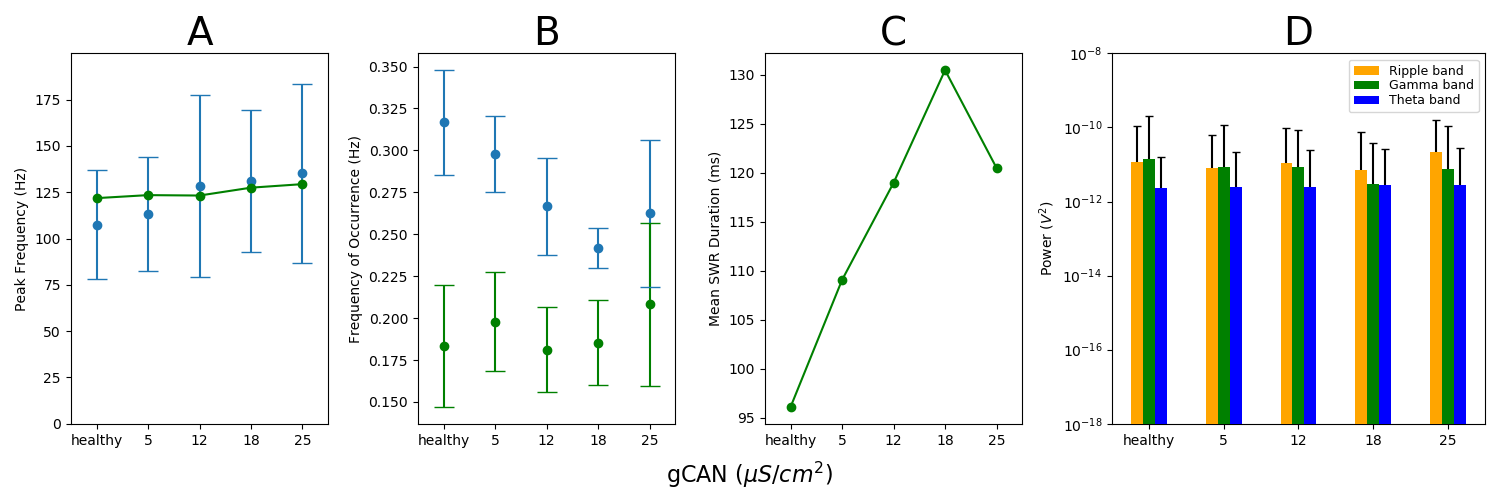
\includegraphics[width=1\linewidth]{images/attack_results/gCAN.png}
            \caption{The impact of \textbf{gCAN} on sharp wave ripples. Values across the parameter range are compared to healthy ones, regarding the most important aspects of activity patterns. To derive these results, 8 simulations of 60 seconds were performed for all depicted parameter values. \textbf{A:} Overview of peak frequencies in events. Mean and standard deviation of all events in \textit{blue}. Mean values of those qualifying as sharp wave ripples in \textit{green}. \textbf{B:} Mean and standard deviation of event occurrence frequencies. All events in \textit{blue}, sharp wave ripples in \textit{green}. \textbf{C:} Development of sharp wave ripple durations. \textbf{D:} Mean and standard deviations of the power in different frequency bands (Ripple band = 100-250Hz, Gamma band = 30-100Hz, Theta band = 5-10Hz). Calculated from all event recordings.}
            \label{fig:attack-gCAN}
        \end{figure}
        % discuss most relevant observations
        Figure \ref{fig:attack-gCAN}, shows a collection of plots, that incorporate the most important aspects of the output analysis. Allowing for a range of interesting observations. \textbf{A} indicates for example, that higher values of \textit{gCAN}, lead to an overall increase in the event peak frequency. Rising from the healthy 107Hz to a mean of 135Hz at the top of the parameter range. The largest step, however, takes place from 5 to 12 \(\mu S/cm^2\), where the mean peak already reaches 128 Hz.\\
        This increase is accompanied by an overall decrease in event occurrences (shown in \textbf{B}), although SWR are not affected by this. Their frequency of occurrence increases even. This shows that the increased peak frequency was able to overcompensate for this otherwise negative effect. At least concerning memory consolidation activities.\\
        \textbf{C} allows for the final observation of an increase in the SWR duration. But since this effect leads to a maximum duration that still lies below the values of \textcite{AmelieAussel.2020}, it was not considered an impairment of cognitive function.\\


        \subsubsection{Cholinergic Modulation of Synapse Conductances (gACh)}
        Acetylcholine also influences a series of synaptic conductances, which differ depending on the region (see the design chapter for more details). This cholinergic conductance modulation scales similarly to \textit{gCAN}, with the neurotransmitter concentration. Since the specific effects are more complex, \textit{gACh} only represents a scaling factor, which is translated into the conductance values by the model. The explored parameter range starts with 1 (representing the acetylcholine levels during sleep) and goes up to 3 (to also represent 3 times the neurotransmitter concentration).
        
        \begin{figure}[htbp]
            \centering
            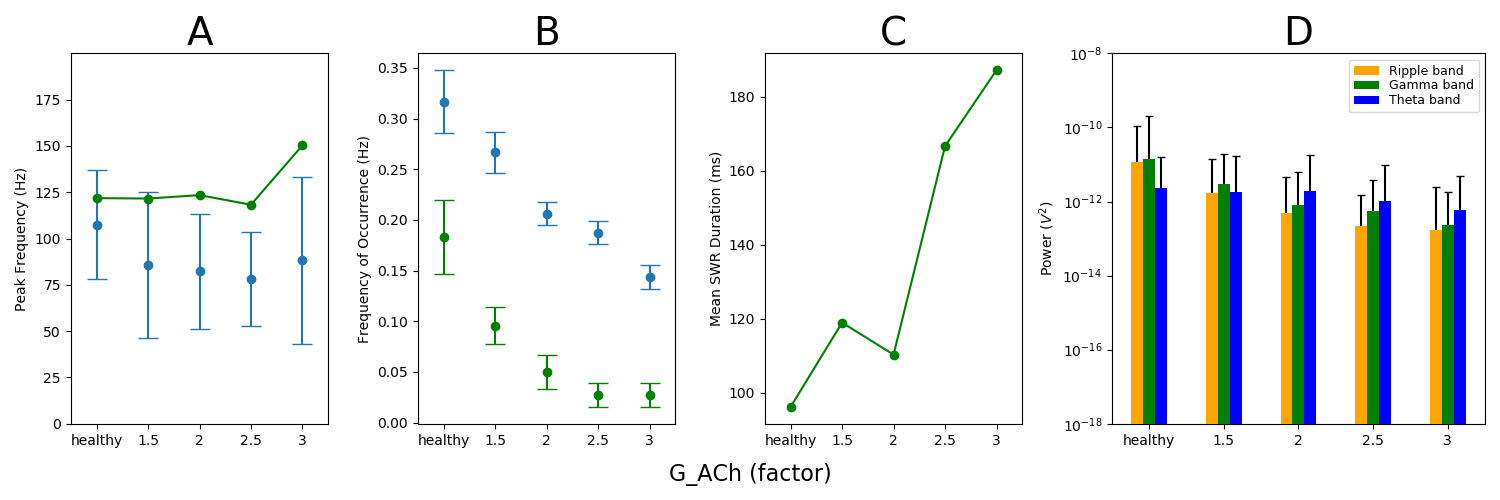
\includegraphics[width=1\linewidth]{images/attack_results/G_ACh.png}
            \caption{The impact of \textbf{gACh} on sharp wave ripples. See figure \ref{fig:attack-gCAN} for a detailed explanation. This data was derived and presented in the same fashion. Only the investigated parameter differs.}
            \label{fig:attack-gACh}
        \end{figure}
        The results presented in figure \ref{fig:attack-gACh}, indicate a notable impact of the parameter on every analyzed aspect. The general peak frequencies of events show already with the smallest increase of \textit{gACh} (to a value of 1.5), a decrease of 22Hz. Since this moves the peak values far outside the ripple frequency range, a reduction of sharp wave ripples is to be expected as a consequence.\\
        As plot \textbf{B} indicates, the reduction of sharp wave ripples, driven by the overall event decrease, indeed seems to be reinforced by this effect. During the first parameter step, the mean of all event occurrences is only reduced by about 15\%, and the number of SWRs is almost halved (from 11 to 5.75 events per minute). Beginning from a \textit{gACh} value of 2.5, the model then seems to reach a low point of SWR occurrence (0.027Hz or 1.625 events per minute). Given that sharp wave ripples play a critical role in memory consolidation \cite{Girardeau.2011}, such extreme values certainly can be associated with an impairment.\\
        Further observations show a strong increase in SWR duration, which in this case also surpasses any reference value. But also a noticeable power decrease across all oscillation bands seems to be related to an increasing value for \textit{gACh}.


        \subsubsection{Overall Effect of Acetylcholine}
        To simulate the compound effect of elevated acetylcholine levels in the hippocampus, the above-explored parameters were simultaneously adjusted. This was done by combining values that reflect a similar neurotransmitter concentration in the network. Through this, it was possible to simulate varying levels of acetylcholine in the model and observe their overall effects on memory consolidation.

        \begin{figure}[htbp]
            \centering
            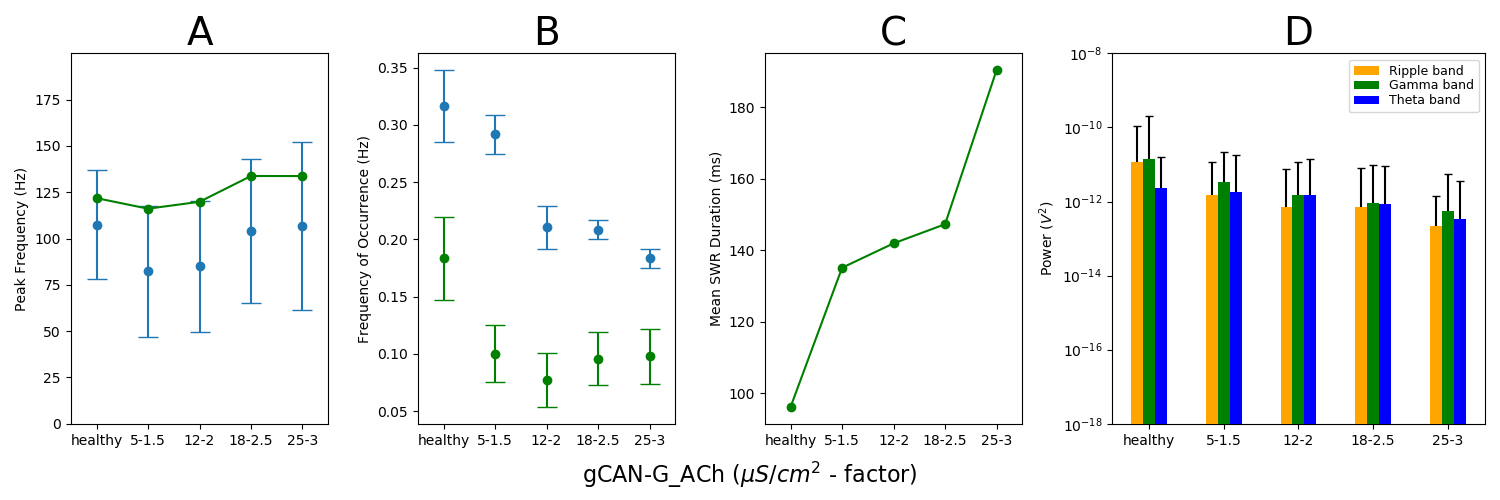
\includegraphics[width=1\linewidth]{images/attack_results/gCAN-G_ACh.png}
            \caption{The overall impact of \textbf{acetylcholine} on sharp wave ripples. See figure \ref{fig:attack-gCAN} for a detailed explanation. This data was derived and presented in the same fashion. Only the investigated parameters differ.}
            \label{fig:attack-acetylcholine}
        \end{figure}
        The combination of both parameters produced a result, in which most values lie between the ones of the individual parameters. But since the parameter \textit{gACh}, generally showed effects of larger magnitude, it tends to dominate the combined effect.\\
        This is well illustrated by the event occurrence frequencies, depicted in plot \textbf{B}. Whilst the results related to \textit{gCAN} (see figure \ref{fig:attack-gCAN}) indicated a (small) increase of SWR occurrences, the combined simulation results are way more similar to the (strong) decrease, that was shown with \textit{gACh} (see figure \ref{fig:attack-gACh}).\\
        A similar observation can be made regarding SWR durations (plot \textbf{C}) and event powers (plot \textbf{D}). Only in the aspect of event peak frequencies, where both parameters show a similar effect strength, are the results more balanced between the two influences.

        The influence of acetylcholine on memory consolidation, therefore seems to be driven by the cholinergic modulation of synaptic conductances (parameter \textit{gACh}). Overall showing a clear impact on SWRs, even at the smallest simulated deviation of the healthy sleep values. Especially the large reduction of SWR occurrences is of concern for memory consolidation. Whilst the healthy state produces 11 events in a minute, no simulated attack values allow for more than 6.\\
        Changes in acetylcholine, therefore represent a mechanism that could indeed be involved in the learning and memory impairments, reported by victims of NeuroStrikes. 
        

        
    \subsection{Structural Damage}
    % What does this section analyze
        % Electromagnetic Attack
        % by simulating a different effect of it on the network
        % Structural damage
    % How was this done
        % was represented by two parameters that reflect such damage
        % Reduction of Neurons
        % Reduction of excitatory synapse conductance
    % Mention structure of approach and section
    This section evaluates a different effect of RF EMR on the hippocampus and its implications on memory consolidation. More precisely, structural damage was simulated by adjusting parameters that reflect either neuron or synapse damage. Exploring these parameters across a range of values, allowed for their assessment in different degrees of severity.\\
    The following analysis is structured very similarly to the previous section, where both parameters are analyzed on their own before their compound effect is assessed.

    
        \subsubsection{Neuronal Damage (N)}
        % Parameter description
        Neuron damage was integrated into the model by reducing the amount of simulated neurons. This was done by adjusting the reference parameter \textit{N}, which specifies the number of neurons in a region of the network and scales the others as specified in the design section. It was explored with a healthy value of 10'000, and across a range that at its lowest value of 6'000 represents a 40\% neuron decrease.

        % Results
        \begin{figure}[htbp]
            \centering
            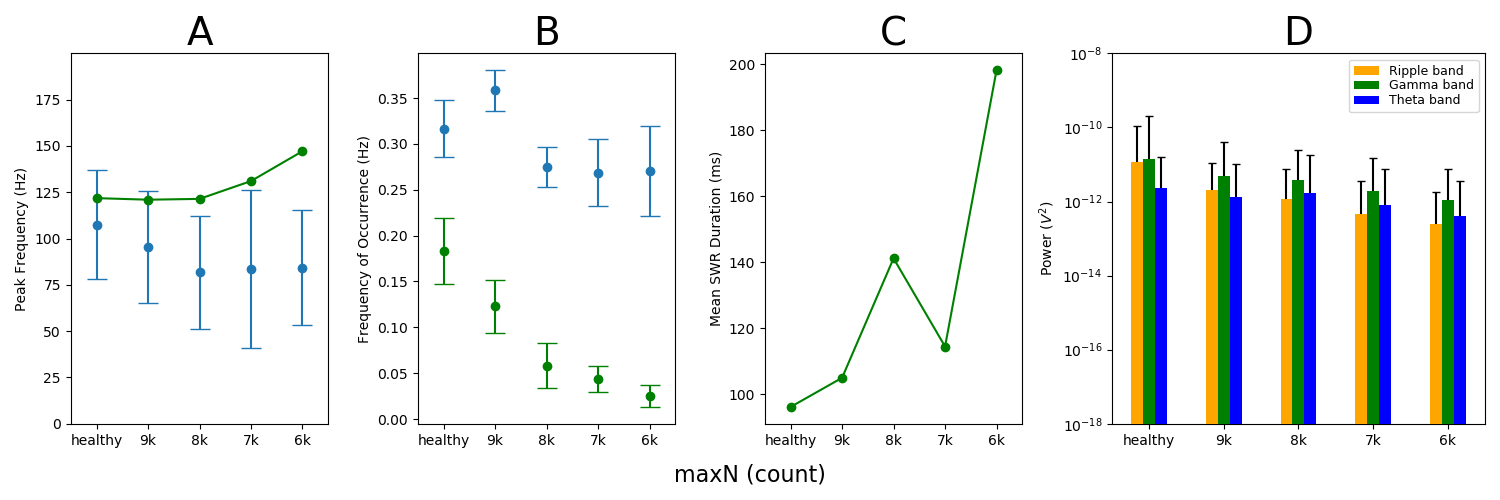
\includegraphics[width=1\linewidth]{images/attack_results/maxN.png}
            \caption{Impact of \textbf{N} on sharp wave ripples. See figure \ref{fig:attack-gCAN} for a detailed explanation. This data was derived and presented in the same fashion. Only the investigated parameter differs.}
            \label{fig:attack-neuron}
        \end{figure}
        % Evaluation of results
        The effect of a neuron reduction is relatively consistent for every step of the simulated parameter range. Ultimately resulting in severe alterations of event-related aspects.\\
        Whilst the general event occurrence remains on a similar level, the peak frequencies of the occurring events are reduced to mean values of about 80Hz. In turn, almost none of them qualify as SWRs, as plot \textbf{B} indicates.
        \begin{figure}[htbp]
            \centering
            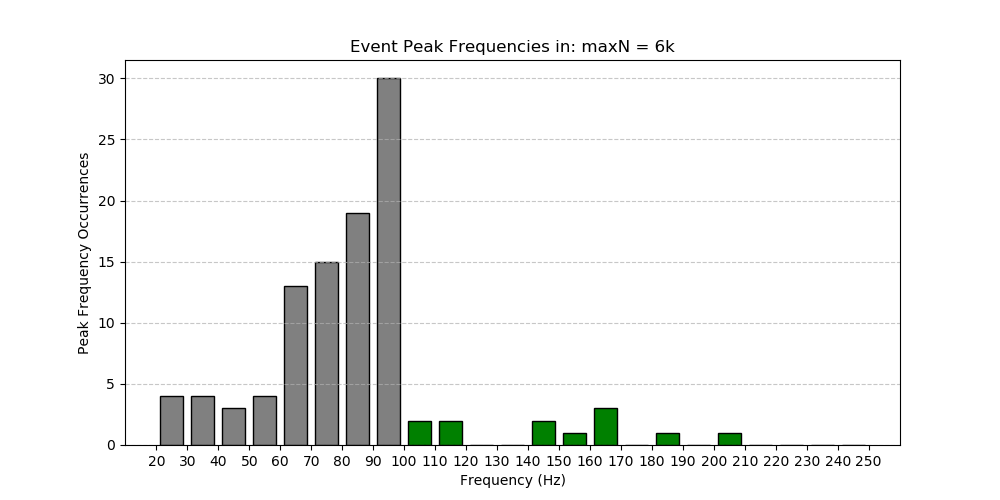
\includegraphics[width=0.75\linewidth]{images/attack_results/maxN-6k-dist.png}
            \caption{Peak frequency distribution, with a configuration of \textit{N} = 6. Showing the absolute value of event occurrences in the indicated frequency bands of 10Hz width, derived from 8 simulations of 60 seconds. Sharp wave ripple events are depicted in \textit{green}, others in \textit{grey}.}
            \label{fig:attack-neuron-6k}
        \end{figure}
        However, as figure \ref{fig:attack-neuron-6k} shows, many events fall just below the peak frequency range to qualify as SWR. This shows that this rather strong effect does to some degree depend on the exact definition of the ripple frequency range. Nonetheless, the range employed by this work is already very broad, and almost no encountered definitions, would consider lower values for ripples.\\ 
        The observed reduction of SWRs was therefore still considered to be relevant. In combination with the large increase in their duration and loss of power, the parameter certainly has a strong influence on SWRs and therefore might impair memory consolidation processes. 
        
        
        \subsubsection{Synaptic Damage (g\_max\_e)}
        Synapse damage was explored, by integrating associated reductions of synaptic conductances into the model. This was achieved by adjusting parameter \textit{g\_max\_e}, which controls the maximum conductances of all excitatory synapses in the network. Its healthy value was defined as \(60pS\) whilst the lower bound of the explored parameter range was chosen at a 20\% reduced value of \(48pS\).
        
        % Results
        \begin{figure}[htbp]
            \centering
            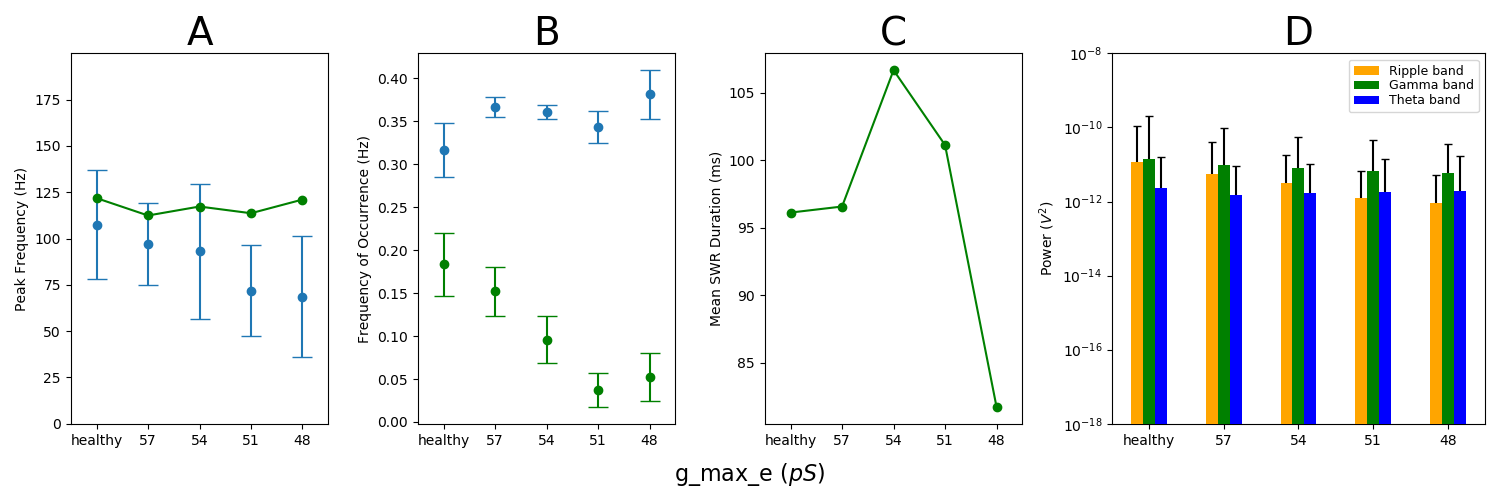
\includegraphics[width=1\linewidth]{images/attack_results/g_max_e.png}
            \caption{The impact of \textbf{g\_max\_e} on sharp wave ripples. See figure \ref{fig:attack-gCAN} for a detailed explanation. This data was derived and presented in the same fashion. Only the investigated parameters differ.}
            \label{fig:attack-g_max_e}
        \end{figure}
        The influence seems to follow the general trend of simulated attack parameters, which manifests itself as a reduction of the overall peak frequency of detected events. \textit{g\_max\_e} does however show a comparably strong influence on these event oscillations. The otherwise increasingly occurring events are therefore not qualifying as SWR. Leading to an overall reduction, that ultimately results in a SWR occurrence frequency of \textit{0.05Hz}.\\
        Besides this, \textit{g\_max\_e} shows a unique effect on the duration of events. Unlike any other analyzed parameter, it reduces the duration of SWRs. At least with the most extreme value of \textit{48pS}, a mean duration of only 82ms was observed.\\
        Whilst the decrease in sharp wave ripples already indicates a reduced memory consolidation activity, the shorter event duration can also be associated with an impairment of the process \cite{Samanta.2023}.
        
        
        \subsubsection{Overall Effect of Structural Damage}
        To assess the overall impact of structural damage on memory consolidation, the above two, individually analyzed parameters, were simultaneously adjusted. In this process, parameter values were matched that were relative to their explored ranges of similar severeness, to represent a coherent radiation state of the brain.
        
        % Results
        \begin{figure}[htbp]
            \centering
            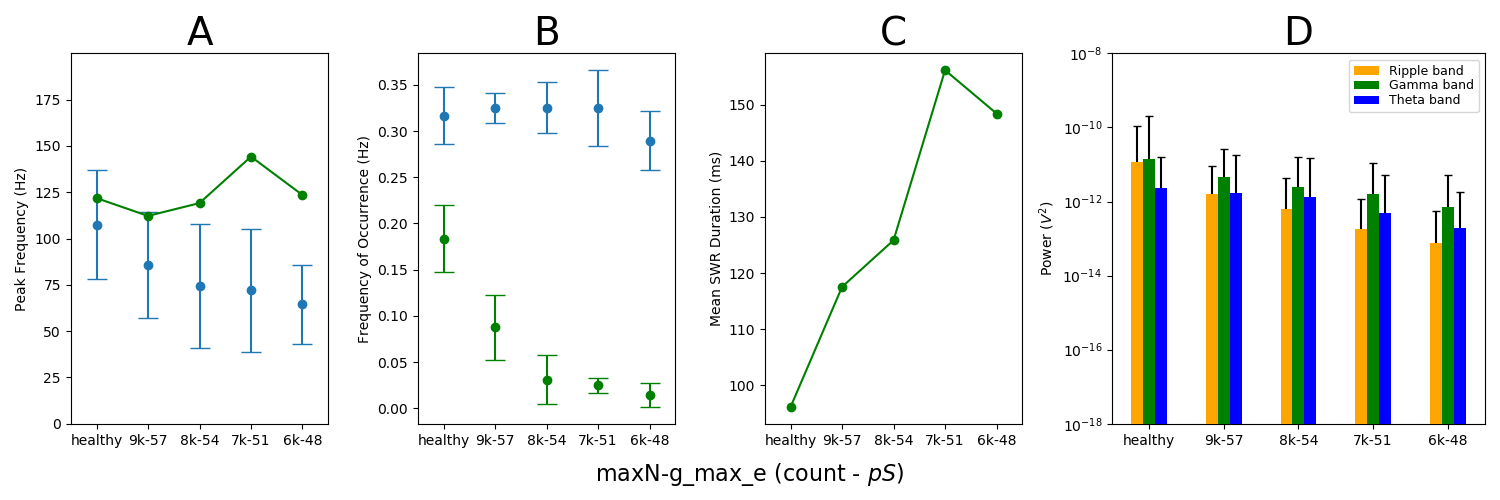
\includegraphics[width=1\linewidth]{images/attack_results/maxN-g_max_e.png}
            \caption{The overall impact of \textbf{structural damage} on sharp wave ripples. See figure \ref{fig:attack-gCAN} for a detailed explanation. This data was derived and presented in the same fashion. Only the investigated parameters differ.}
            \label{fig:attack-structural_damage}
        \end{figure}
        % Evaluation of Results
        The two included parameters produced similar results in their isolated analysis. Their combination, however, yielded results that show more extreme values, than any component. Indicating a reinforcement effect between the two.\\
        This leads to extraordinarily low values in the general peak frequencies, which are as expected, accompanied by a low number of SWRs. Whilst the SWR duration is only increased to similar levels as mentioned by \textcite{AmelieAussel.2020}, the power in all observed oscillation bands reaches relatively low values.

        Considering these observations in the context of memory consolidation, the implications are clear. With less than one sharp wave ripple occurring per minute (0.01Hz), it is to be expected that the cognitive process is impaired. Especially when also considering the other aspects. Structural damage should therefore also be considered as a potential underlying mechanism involved in the symptoms of electromagnetic attacks.


    \subsection{Full Attack}
    The following section is concerned with evaluating a \textit{full attack}, that incorporates both, neurotransmitter changes and structural damage. Like this, a more complex scenario was created, in which multiple mechanisms were employed at the same time, to represent the effects of an electromagnetic attack more realistically.\\
    To achieve this, all 4 previously presented parameters were altered simultaneously. Following the approach that was elaborated in the design section, where 4 different levels of attack intensity were explored.\\

    % Results
    \begin{figure}[htbp]
        \centering
        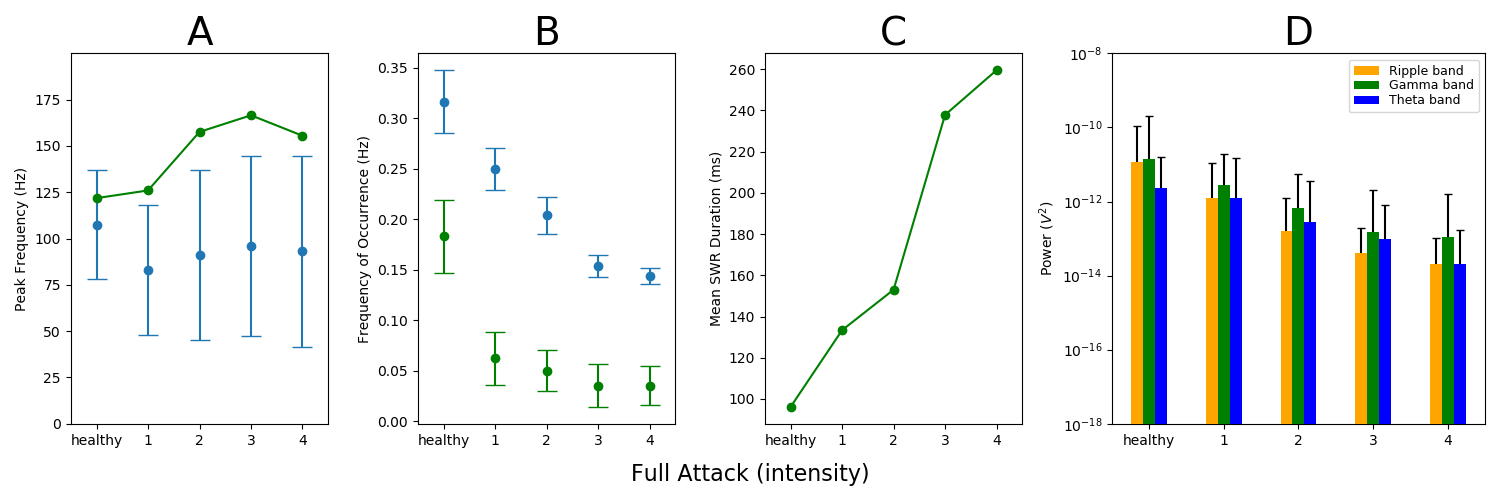
\includegraphics[width=1\linewidth]{images/attack_results/Full Attack.png}
        \caption{The impact of a \textbf{full scale attack} on sharp wave ripples. See figure \ref{fig:attack-gCAN} for a detailed explanation of the plots. This data was derived and presented in the same fashion. Parameter values at each intensity level for \textbf{(N, g\_max\_e, gCAN, gACh)} were chosen as follows: \textbf{1:} (9k-57-5-1.5), \textbf{2:} (8k-54-12-2), \textbf{3:} (7k-51-18-2.5), \textbf{4:} (6k-48-25-3).}
        \label{fig:attack-Full}
    \end{figure}
    The general result pattern does reflect the characteristics of its components. Especially considering the overall results of neurotransmitters and structural damage. Some aspects however appear only in this combined simulation.\\
    As for all attack-related results, except for those of \textit{gCAN}, the event peak frequency and occurrence of SWRs are reduced. Further indicating their connection. 
    Although the mean value of the peak frequencies does not drop far, the SWR occurrence frequency quickly reaches values around 0.05Hz. This might, however, be related to the peak frequencies' consistently large standard deviation.\\
    Most remarkable is nonetheless the SWR duration, which reaches a peak value of 238ms and thereby surpasses any reference values. But these results also incorporate the strongest decrease in power across all oscillation bands.\\

    Considering these results, a very apparent disruption of healthy SWRs can be observed. Most importantly their occurrence frequency quickly drops to about a quarter of its healthy sleep value. Suggesting that already an attack inducing the smallest intensity of alterations in the brain could disrupt memory consolidation processes. Such effects would then most likely only be reinforced with rising intensity levels since the oscillation power and SWR duration keep deviating from the healthy range.\\
    This more complex scenario could therefore already with less severe radiation exposures and resulting alterations in the brain, play a role in the learning and memory impairments of NeuroStrikes. Overall this can be considered the most robust and probable representation of an electromagnetic attack. 
    
    

% General Pattern Section beginning:
    % What was analyzed
        % Integrate in context of the work
    % How was that performed
        % keep it short and precise, no theoretical explanations
        % just motivate the approach
        % draw connection to what changes the attack configurations represent in the brain
    % Give overview of following analysis

% Subsection/Data Presentation:
    % Specifying high level meaning of parameter
        % Present parameter range
            % connect with meaning (0.5 sleep concentration, 25 waking concentration)
        % Plot
            % describe thoroughly once
            % then reference for explanation
        % discuss most relevant observations
        % relate to memory consolidation

% How could that be interpreted
\chapter{Final Considerations}
\label{chap:considerations}

%Regarding Final Considerations:
% I. Some teachers and/or methods use the term Conclusion for a text at the end of the paper that aims to expose the results achieved, this term is not incorrect, but many of the works are bibliographical reviews where in the end no conclusion is obtained and yes Several considerations that were found in the development of written work. Therefore, in each project should be considered/weighted if there will be a Conclusion or Final Considerations. Usually what else happens is that you have Final Considerations. The Final Considerations of a paper aims to show if the goal sought for the project was achieved, as well as give a view of the most important considerations and conclusions on the subject addressed, among other aspects. This should include:
%Summary
%1. An explanation stating clearly whether or not it has achieved the stated objectives (a subdivision between general objectives and specific objectives can also be made here). In each case the reasons must be explained:
%The. If you have achieved the objectives: inform the main factors that contributed to the success, describing them briefly, but do not leave doubts;
%B. If you have not met the objectives: inform how much of the objective has been achieved and cite the factors that contributed to the failure, describing them briefly, but that leaves no doubt.
%Considerations
%2. Describe the main considerations and conclusions that were obtained as a result of the execution of the work. Here should not be repeated text already in the work, but write the impressions of these considerations and how they contributed to the implementation and achieved the goal;
%3. Name and describe the main difficulties encountered in the execution of the work and project. All the work developed means an evolution for the student, and to reach this evolution, it has had to overcome a series of obstacles. Reporting obstacles and overcoming (or not overcoming) helps to dignify and show the merit of the work itself to the reader/evaluator. It is also a contribution, in the sense that once problems and solutions are exposed, readers/evaluators learn/know ways of solving or approaching such problems;
%4. Discuss whether modifications occurred during the execution of the work within the scope defined in the Project phase and in what was developed. It should be explained what generated those modifications, substantiating and justifying such changes.
%5. The relationship between the proposed schedule and the work schedule can be described. This allows the reader/evaluator to learn from the indicated distortions/hits.
%Future Work
%6. Describe or cite future work that may be done based on this work. During the execution of work, it is sought to reach a defined objective in the project. However, several interesting subjects of research are revealed (being that the same ones are not treated/researched in the work because they do not match the objective and scope of the work). The description of such subjects/themes/research demonstrates the students' perception of development as well as their vision of objectivity in the execution of this work.

%II. Conclusion / Final Considerations aim to show the reader/evaluator the student's perception of the work done. In this way, it is not advisable to do citations and references because theoretically everything that was necessary to quote and refer should already be done within the content of the work. Only in some very specific cases/situations can you make referrals or citations in this part of the work (this should be discussed thoroughly with the supervisor/teacher).

%III. Looking at the described items that should compose the Conclusion / Final Considerations, it is difficult to imagine that this part of the work has less than one page;

This final chapter supplies a conclusive overview, of the performed work. First, providing a comprehensive \textit{Summary} that elaborates on the research process and aims to show the evolution of the work. Then the encountered \textit{Limitations} are revealed before the thesis goals and related insights are discussed in the \textit{Conclusions}. Finally, some opportunities for \textit{Future Work} are presented. 
 


\section{Summary}
% I did this in this way, that in that way... and so on
The core contribution of this work is the identification of potential underlying mechanisms of Electromagnetic attacks. A technological form of cognitive warfare, that has gained a lot of relevance in recent years. Since there even exists a series of health incidents that are associated with such attacks, the importance of a suitable countermeasure is apparent. To propose such a solution based on BCIs was therefore part of the initial goals of the thesis. Due to the extreme novelty of the topic, as well as the simulation nature of the research, it was however not possible to achieve this goal.

This work required background knowledge in a large field of topics, ranging from purely biological subjects to very technical ones. Performing a thorough review of them already revealed a limited amount of literature in the realm of \textit{Cognitive Warfare}, but especially regarding its technological form. This lack of previous work, became even more evident when more specific related work was explored. Against initial expectations, no literature on the underlying mechanisms of electromagnetic attacks (or "NeuroStrikes") could be identified. This led to a shift in the research goal, as such specifics were necessary to develop a countermeasure. Especially since the investigations were performed with the help of simulations, at least a somewhat validated hypothesis on the involved mechanisms and their implementation, was a requirement for any further work.\\
Additional investigations were therefore performed on the technological basis of electromagnetic attacks, which is considered to be radio-frequency electromagnetic radiation. Setting a special focus on its effects on the brain. This revealed a set of neurological alterations that could be responsible for cognitive impairments that were observed in the context of Neurostrikes.

Due to the scale of this work, it was only feasible to investigate the impairment and potential causes, of a single cognitive process. In parts, because the identification and configuration of a simulation model, related to a relevant cognitive process, is very time-consuming. It was nonetheless possible, to identify a suitable model of the hippocampus, that enabled investigations of memory consolidation. To produce realistic brain activity with this model, it was however necessary to further provide a realistic simulation input. But also the development of an output analysis was required, to evaluate the simulated performance of memory consolidation. These two aspects bear enough complexity to perform dedicated research on them, and therefore could not be investigated to their full extent.\\
A synthetic approach to the input generation was nonetheless explored, which turned out to be quite difficult if realism is of concern. Fortunately, it was possible to obtain EEG files from the model creator, which allowed for a realistic representation of the input activity. Also regarding the output analysis, a general approach could be derived from previous work on the model. This established the necessary foundation to utilize the simulation model, for the investigations of interest. 

 To assess the potential underlying mechanisms of electromagnetic attacks, simulations were performed in two stages. First, the healthy model behavior was observed and documented, to establish reference values for the relevant output aspects. Then a series of potentially attack-related alterations were integrated into the model, which had a large impact on the analyzed behavior. Yielding values, that in most cases showed a clear disruption of healthy memory consolidation activities.


\section{Limitations}
% General research:
% Too far of a step, outside of work done so far
        % Too many aspects needed for the work are still not established -> difficult to establish solid research foundation
It has to be considered that this thesis explored a very novel and poorly researched subject. The lack of related work, sometimes only could be supplemented with literature and findings, that were derived from different contexts. This required assumptions regarding their validity across contexts and made it a complex task to establish a solid research foundation.

% Simulations:
% limitations regarding Output analysis
    % Many parameter definitions vary massively
    % Depending on parameters, very different results
    % optimization and evaluation is a work of its own
% Constraint of Computing Power
Further, some limitations regarding the simulation work must be stated. Even though the influence of the output analysis on the result values is large, it was not possible to validate the developed approach to the full extent. This makes claims about its accuracy difficult. Additionally due to inconsistent definitions in the literature, regarding key aspects of the analyzed output (like the ripple frequency range), the comparability to other results might be limited.


\section{Conclusions}
% Lessons learned
This section concludes the work, by elaborating on the initially defined objectives, to show what was achieved and learned in the process.

% Simulator
Throughout the work, it was possible to identify and configure, a suitable \textbf{simulation model} that produced mostly realistic behavior in its healthy state. It must however be stated that this process came with a lot of obstacles and uncertainties that were not anticipated. Already the identification of an appropriate model proved to be challenging. Above all,  obtaining a realistic input posed a complex problem, which without the support and provision of EEG files by the model creator would have been difficult to solve reliably. Overall, it should not be underestimated how time-consuming the work with brain simulators can be.

% Electromagnetic attack mechanisms
In the context of \textbf{electromagnetic attacks} and their underlying mechanisms, some promising findings could be made. The simulated increase of acetylcholine, as well as the structural damage to the hippocampus, led to remarkable alterations in the observed activity patterns associated with memory consolidation. These mechanisms, and especially their combination, could therefore be involved in attack-related impairments and should consequently also be considered in the development of a countermeasure.

% Countermeasures
Whilst it was not possible, to address the subject of a \textbf{countermeasure} in the scope of this thesis, some initial findings could be made that might contribute to their future development. This includes observations regarding the relationship between brain stimulation and cognitive processes. Most importantly, however, this work contributes to a better understanding of electromagnetic attacks, to help mitigate them. 


\section{Future Work}
As stated in the summary already, especially two topics were encountered throughout the work, that hold the potential for further work.
% Realistic synthetic input
Including first of all the synthetic input generation. As documented, the input has a large influence on the simulation behavior and needs to be realistic to produce relevant activity. Such works could for example explore different input equations or integration methods.\\
% Optimize Sharp Wave ripple identification
As a further research topic, the output analysis was identified. Specifically, the automated detection of sharp-wave ripples in local field potential recordings lacks a solid research foundation and would benefit from a more sophisticated and validated procedure.\\
% Countermeasures based on Brain computer interfaces
    % Mention why it could have potential and might help
Lastly, the original goal of this work, a countermeasure for electromagnetic attacks, remains a mostly unexplored but relevant topic. It does however still require a better understanding of the mechanisms involved in electromagnetic attacks. Even though, this work was able to perform explorations in the realm of memory consolidation, many more cognitive aspects are affected by the attacks. Further research should therefore be conducted to develop a more comprehensive understanding of their mechanisms, such that a countermeasure can be designed appropriately. 

    
   
% --------------
% End
% --------------

% Use the bibtex style (check the file "references.bib").

\addcontentsline{toc}{chapter}{Bibliography}
\sloppy % url line breaks in bibliography
\printbibliography
% --------------
\chapter*{Abbreviations}
\addcontentsline{toc}{chapter}{Abbreviations}
\markboth{ABBREVIATONS}{}


\abr{EMR}{Electromagnetic Radiation}
\abr{RF}{Radio Frequency}
\abr{BCI}{Brain-Computer Interface}
\abr{SWR}{Sharp Wave Ripples}
\abr{EC}{Entorhinal Cortex}
\abr{DG}{Denate Gyrus}
\abr{EEG}{Electroencephalography}
\abr{RMS}{Root Mean Square}
\abr{SD}{Standard Deviation}
\abr{LFP}{Local Field Potential}











% \chapter*{Glossary}
\addcontentsline{toc}{chapter}{Glossary}
\markboth{GLOSSARY}{}

% This item is optional in the thesis

%\begin{description}
%  \item[Authorization] Authorization is the decision whether an entity is allowed to perform a particular action or not, 
%       e.g. whether a user is allowed to attach to a network or not.
%\end{description}
  <- optional
% --------------
\addcontentsline{toc}{chapter}{List of Figures}
\listoffigures
\addcontentsline{toc}{chapter}{List of Tables}
\listoftables
\addcontentsline{toc}{chapter}{List of Listings}
\lstlistoflistings



%\appendix

\chapter{Contents of the Repository}

The code repository contains the following content:

\textbf{Installation} 

%Instructions/README to deploy the prototype


\textbf{Operation} 

%How to run/execute experiments




\end{document}
